\documentclass{beamer}
\usepackage[utf8]{inputenc}
\usepackage{graphicx, epsfig}
\usepackage{amsmath,mathrsfs,amsfonts,amssymb}
%\usepackage{subfig}
\usepackage{floatflt}
\usepackage{epic,ecltree}
\usepackage{mathtext}
\usepackage{fancybox}
\usepackage{fancyhdr}
\usepackage{multirow}
\usepackage{enumerate}
\usepackage{epstopdf}
\usepackage{multicol}
\usepackage{algorithm}
\usepackage[noend]{algorithmic}
\usepackage{tikz}
\usepackage{blindtext}
\usetheme{default}%{Singapore}%{Warsaw}%{Warsaw}%{Darmstadt}
\usecolortheme{default}
\setbeamerfont{title}{size=\Huge}
\setbeamertemplate{footline}[page number]{}


\makeatletter
\newcommand\HUGE{\@setfontsize\Huge{35}{40}}
\makeatother    

\setbeamerfont{title}{size=\HUGE}
\beamertemplatenavigationsymbolsempty

% latin bold lower
\newcommand{\ba}{\mathbf{a}} 
\newcommand{\bc}{\mathbf{c}} 
\newcommand{\be}{\mathbf{e}} 
\newcommand{\bh}{\mathbf{h}} 
\newcommand{\bp}{\mathbf{p}} 
\newcommand{\bt}{\mathbf{t}} 
\newcommand{\bs}{\mathbf{s}} 
\newcommand{\bu}{\mathbf{u}} 
\newcommand{\bv}{\mathbf{v}} 
\newcommand{\bw}{\mathbf{w}} 
\newcommand{\bx}{\mathbf{x}} 
\newcommand{\by}{\mathbf{y}} 
\newcommand{\bz}{\mathbf{z}} 

% latin bold upper
\newcommand{\bA}{\mathbf{A}} 
\newcommand{\bB}{\mathbf{B}} 
\newcommand{\bC}{\mathbf{C}} 
\newcommand{\bI}{\mathbf{I}} 
\newcommand{\bJ}{\mathbf{J}} 
\newcommand{\bL}{\mathbf{L}} 
\newcommand{\bM}{\mathbf{M}} 
\newcommand{\bQ}{\mathbf{Q}} 
\newcommand{\bT}{\mathbf{T}} 
\newcommand{\bU}{\mathbf{U}} 
\newcommand{\bV}{\mathbf{V}} 
\newcommand{\bW}{\mathbf{W}} 
\newcommand{\bX}{\mathbf{X}} 
\newcommand{\bY}{\mathbf{Y}} 
\newcommand{\bZ}{\mathbf{Z}} 

% latin cal upper
\newcommand{\cG}{\mathcal{G}} 
\newcommand{\cL}{\mathcal{L}} 
\newcommand{\cN}{\mathcal{N}} 
\newcommand{\cS}{\mathcal{S}} 
\newcommand{\cT}{\mathcal{T}} 
\newcommand{\cW}{\mathcal{W}} 
\newcommand{\cX}{\mathcal{X}} 
\newcommand{\cZ}{\mathcal{Z}} 

% latin bb upper
\newcommand{\bbE}{\mathbb{E}} 
\newcommand{\bbI}{\mathbb{I}} 
\newcommand{\bbP}{\mathbb{P}} 
\newcommand{\bbR}{\mathbb{R}} 

% greek bold lower
\newcommand{\bepsilon}{\boldsymbol{\epsilon}} 
\newcommand{\btheta}{\boldsymbol{\theta}} 
\newcommand{\blambda}{\boldsymbol{\lambda}} 
\newcommand{\bpi}{\boldsymbol{\pi}} 
\newcommand{\bmu}{\boldsymbol{\mu}} 
\newcommand{\bsigma}{\boldsymbol{\sigma}} 
\newcommand{\bphi}{\boldsymbol{\phi}} 

% greek bold upper
\newcommand{\bSigma}{\boldsymbol{\Sigma}} 

\DeclareMathOperator*{\argmin}{arg\,min}
\DeclareMathOperator*{\argmax}{arg\,max}

\newcommand{\createdgmtitle}[1]{\title[\hbox to 56mm{Deep Generative Models  \hfill\insertframenumber\,/\,\inserttotalframenumber}]
	{\vspace{1cm} \\ Deep Generative Models \\ {\Huge Lecture #1}}
	\author{Roman Isachenko}
	\institute{
	Moscow Institute of Physics and Technology
	} 
	\date{2022}
}

\newcommand\myfootnote[1]{%
  \tikz[remember picture,overlay]
  \draw (current page.south west) +(1in + \oddsidemargin,0.5em)
  node[anchor=south west,inner sep=0pt]{\parbox{\textwidth}{%
      \rlap{\rule{10em}{0.4pt}}\raggedright\scriptsize \textit{#1}}};}

\newcommand\myfootnotewithlink[2]{%
  \tikz[remember picture,overlay]
  \draw (current page.south west) +(1in + \oddsidemargin,0.5em)
  node[anchor=south west,inner sep=0pt]{\parbox{\textwidth}{%
      \rlap{\rule{10em}{0.4pt}}\raggedright\scriptsize\href{#1}{\textit{#2}}}};}
\createdgmtitle{supplementary}
%--------------------------------------------------------------------------------
\begin{document}
%--------------------------------------------------------------------------------
\begin{frame}[noframenumbering,plain]
%\thispagestyle{empty}
\titlepage
\end{frame}
%=======
\begin{frame}[allowframebreaks]{Outline}
	\tableofcontents
\end{frame}
\AtBeginSection[ ]
{
	\begin{frame}[shrink]{Outline}
		\tableofcontents[currentsection,hideothersubsections]
	\end{frame}
}c
\section{Autoregressive models}
%=======
\subsection{Masked Autoencoder (MADE)}
%=======
\begin{frame}{MADE}
	\begin{itemize}
		\item Vanila autoencoder is not a generative model.
		\item Let mask the weight matrices to make the model generative: $\bW_M = \bW \cdot \bM$.
		\begin{figure}
		    \centering
		    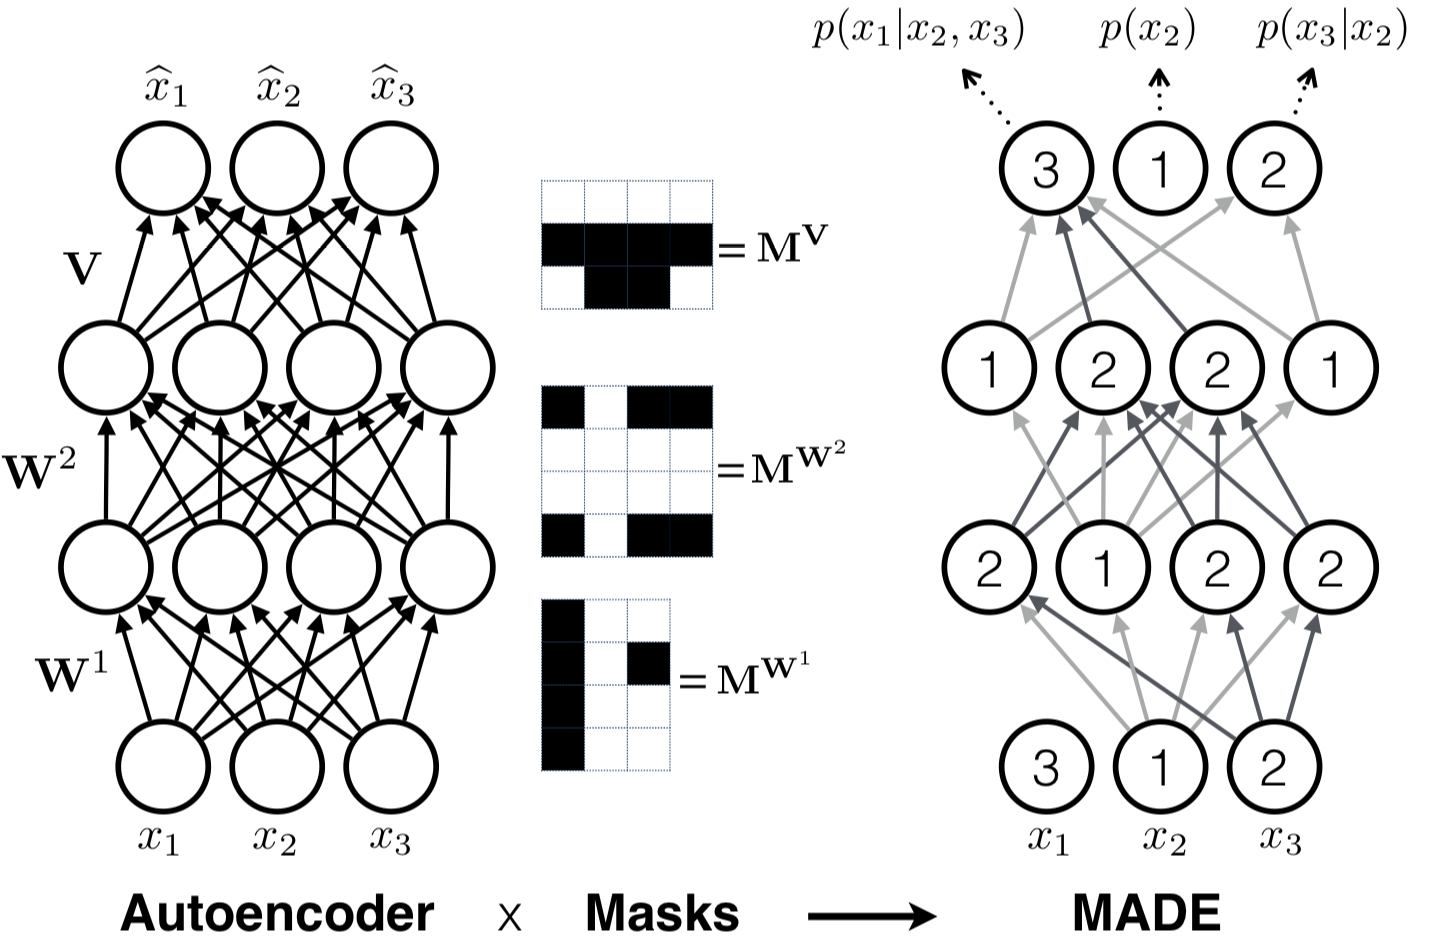
\includegraphics[width=0.7\linewidth]{figs/made}
		\end{figure}
		\item The question is how to create matrices $\bM$ which produce the autoregressive property?
	\end{itemize}
	\myfootnotewithlink{https://arxiv.org/abs/1502.03509}{Germain M. et al. Made: Masked autoencoder for distribution estimation, 2015}
\end{frame}
%=======
\begin{frame}{MADE}
		\begin{minipage}[t]{0.65\columnwidth}
		    \vspace{-0.5cm}
			\begin{block}{Masks generation}
				\begin{itemize}
					\item Define the ordering of input elements from 1 to $m$.
					\item Assign the random number $k$ from 1 to $m - 1$ to each hidden unit. The number gives the
					maximum value of input units to which the unit can be connected.
					\item Connect each hidden unit with number $k$ with the previous layer units which has the number is \textbf{less or equal} than~$k$.
					\item Connect each output unit with number $k$ with the previous layer units which has the number is \textbf{less} than $k$.
				\end{itemize}
			\end{block}
		\end{minipage}%
		\begin{minipage}[t]{0.33\columnwidth}
			\vspace{2cm}
			\begin{figure}
				\centering
				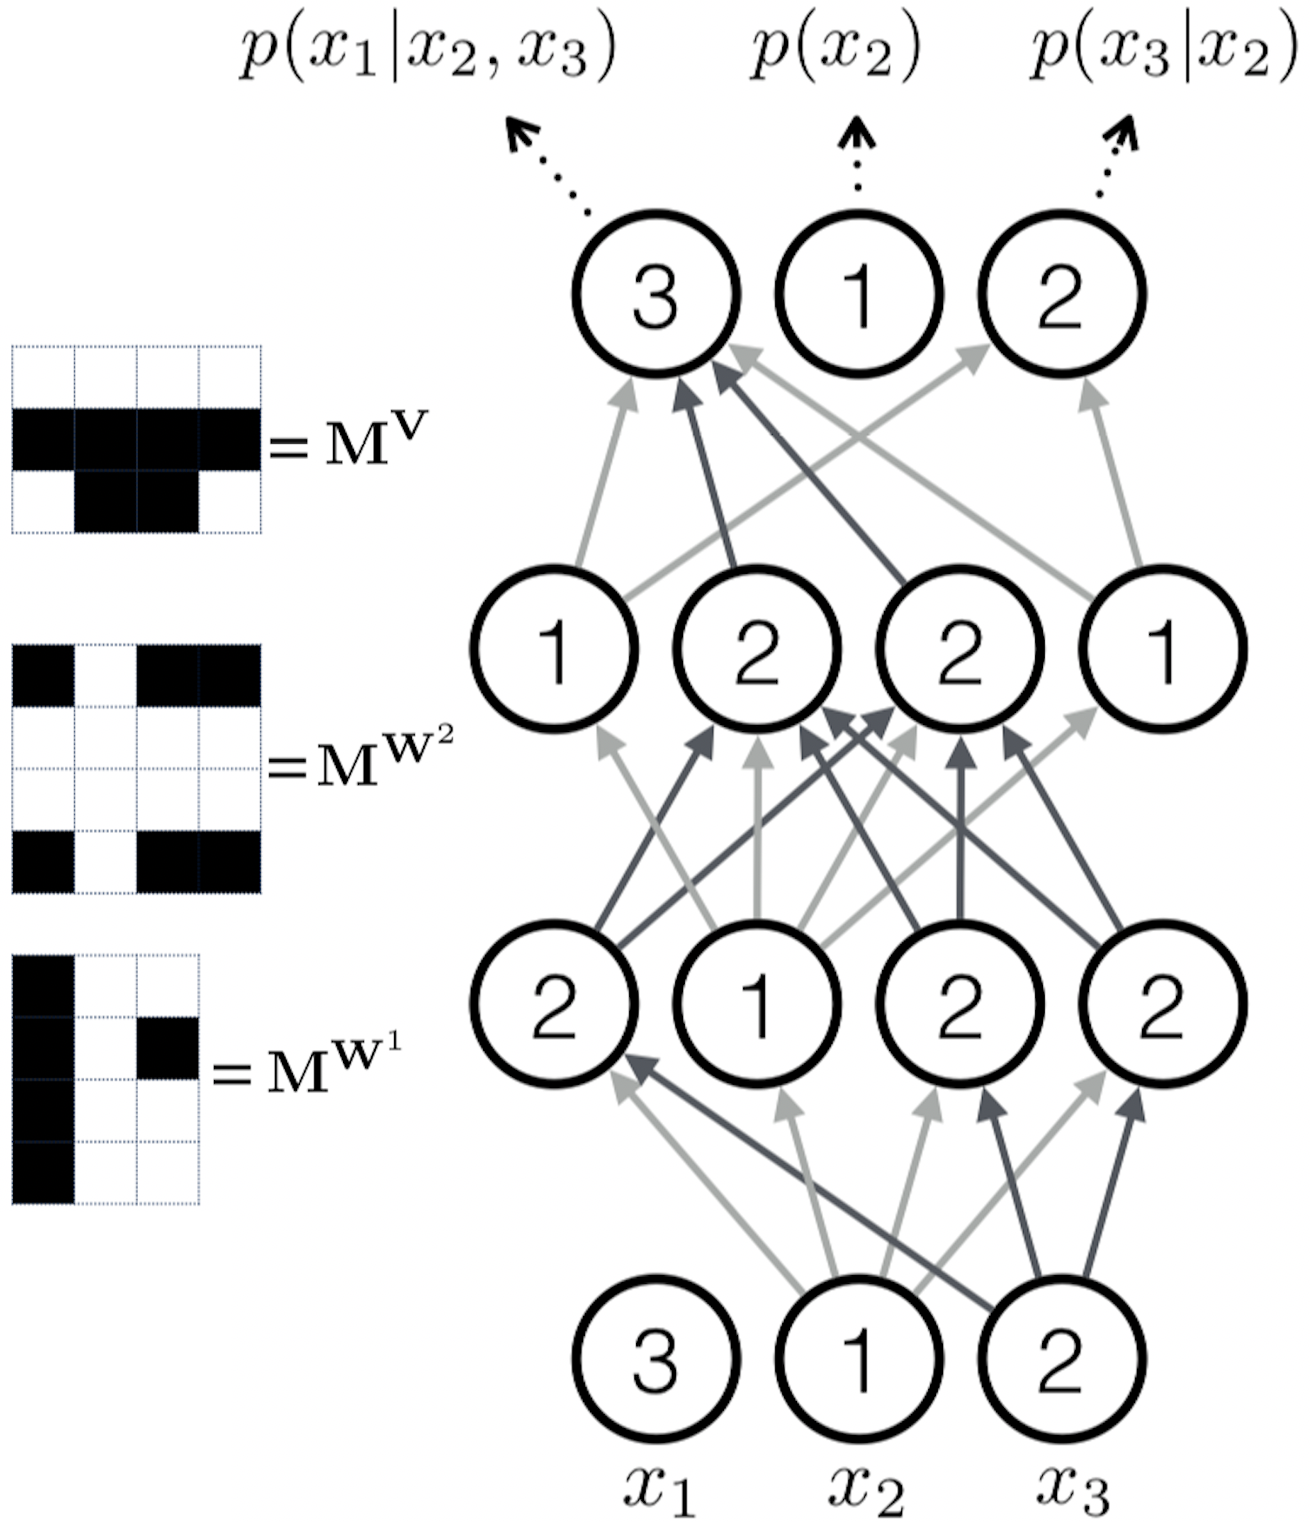
\includegraphics[width=1.0\linewidth]{figs/made2}
			\end{figure}
		\end{minipage}
	\myfootnotewithlink{https://arxiv.org/abs/1502.03509}{Germain M. et al. Made: Masked autoencoder for distribution estimation, 2015}
\end{frame}
%=======
\begin{frame}{MADE}
	\begin{block}{Possible variations}
		\begin{itemize}
			\item Order agnostic training (missing values in partially observed input vectors can be imputed efficiently);
			\item Connectivity-agnostic training (cheap ensembling).
		\end{itemize}
	\end{block}
	\vspace{-0.3cm}
	\begin{minipage}[t]{0.59\columnwidth}
		\begin{figure}
			  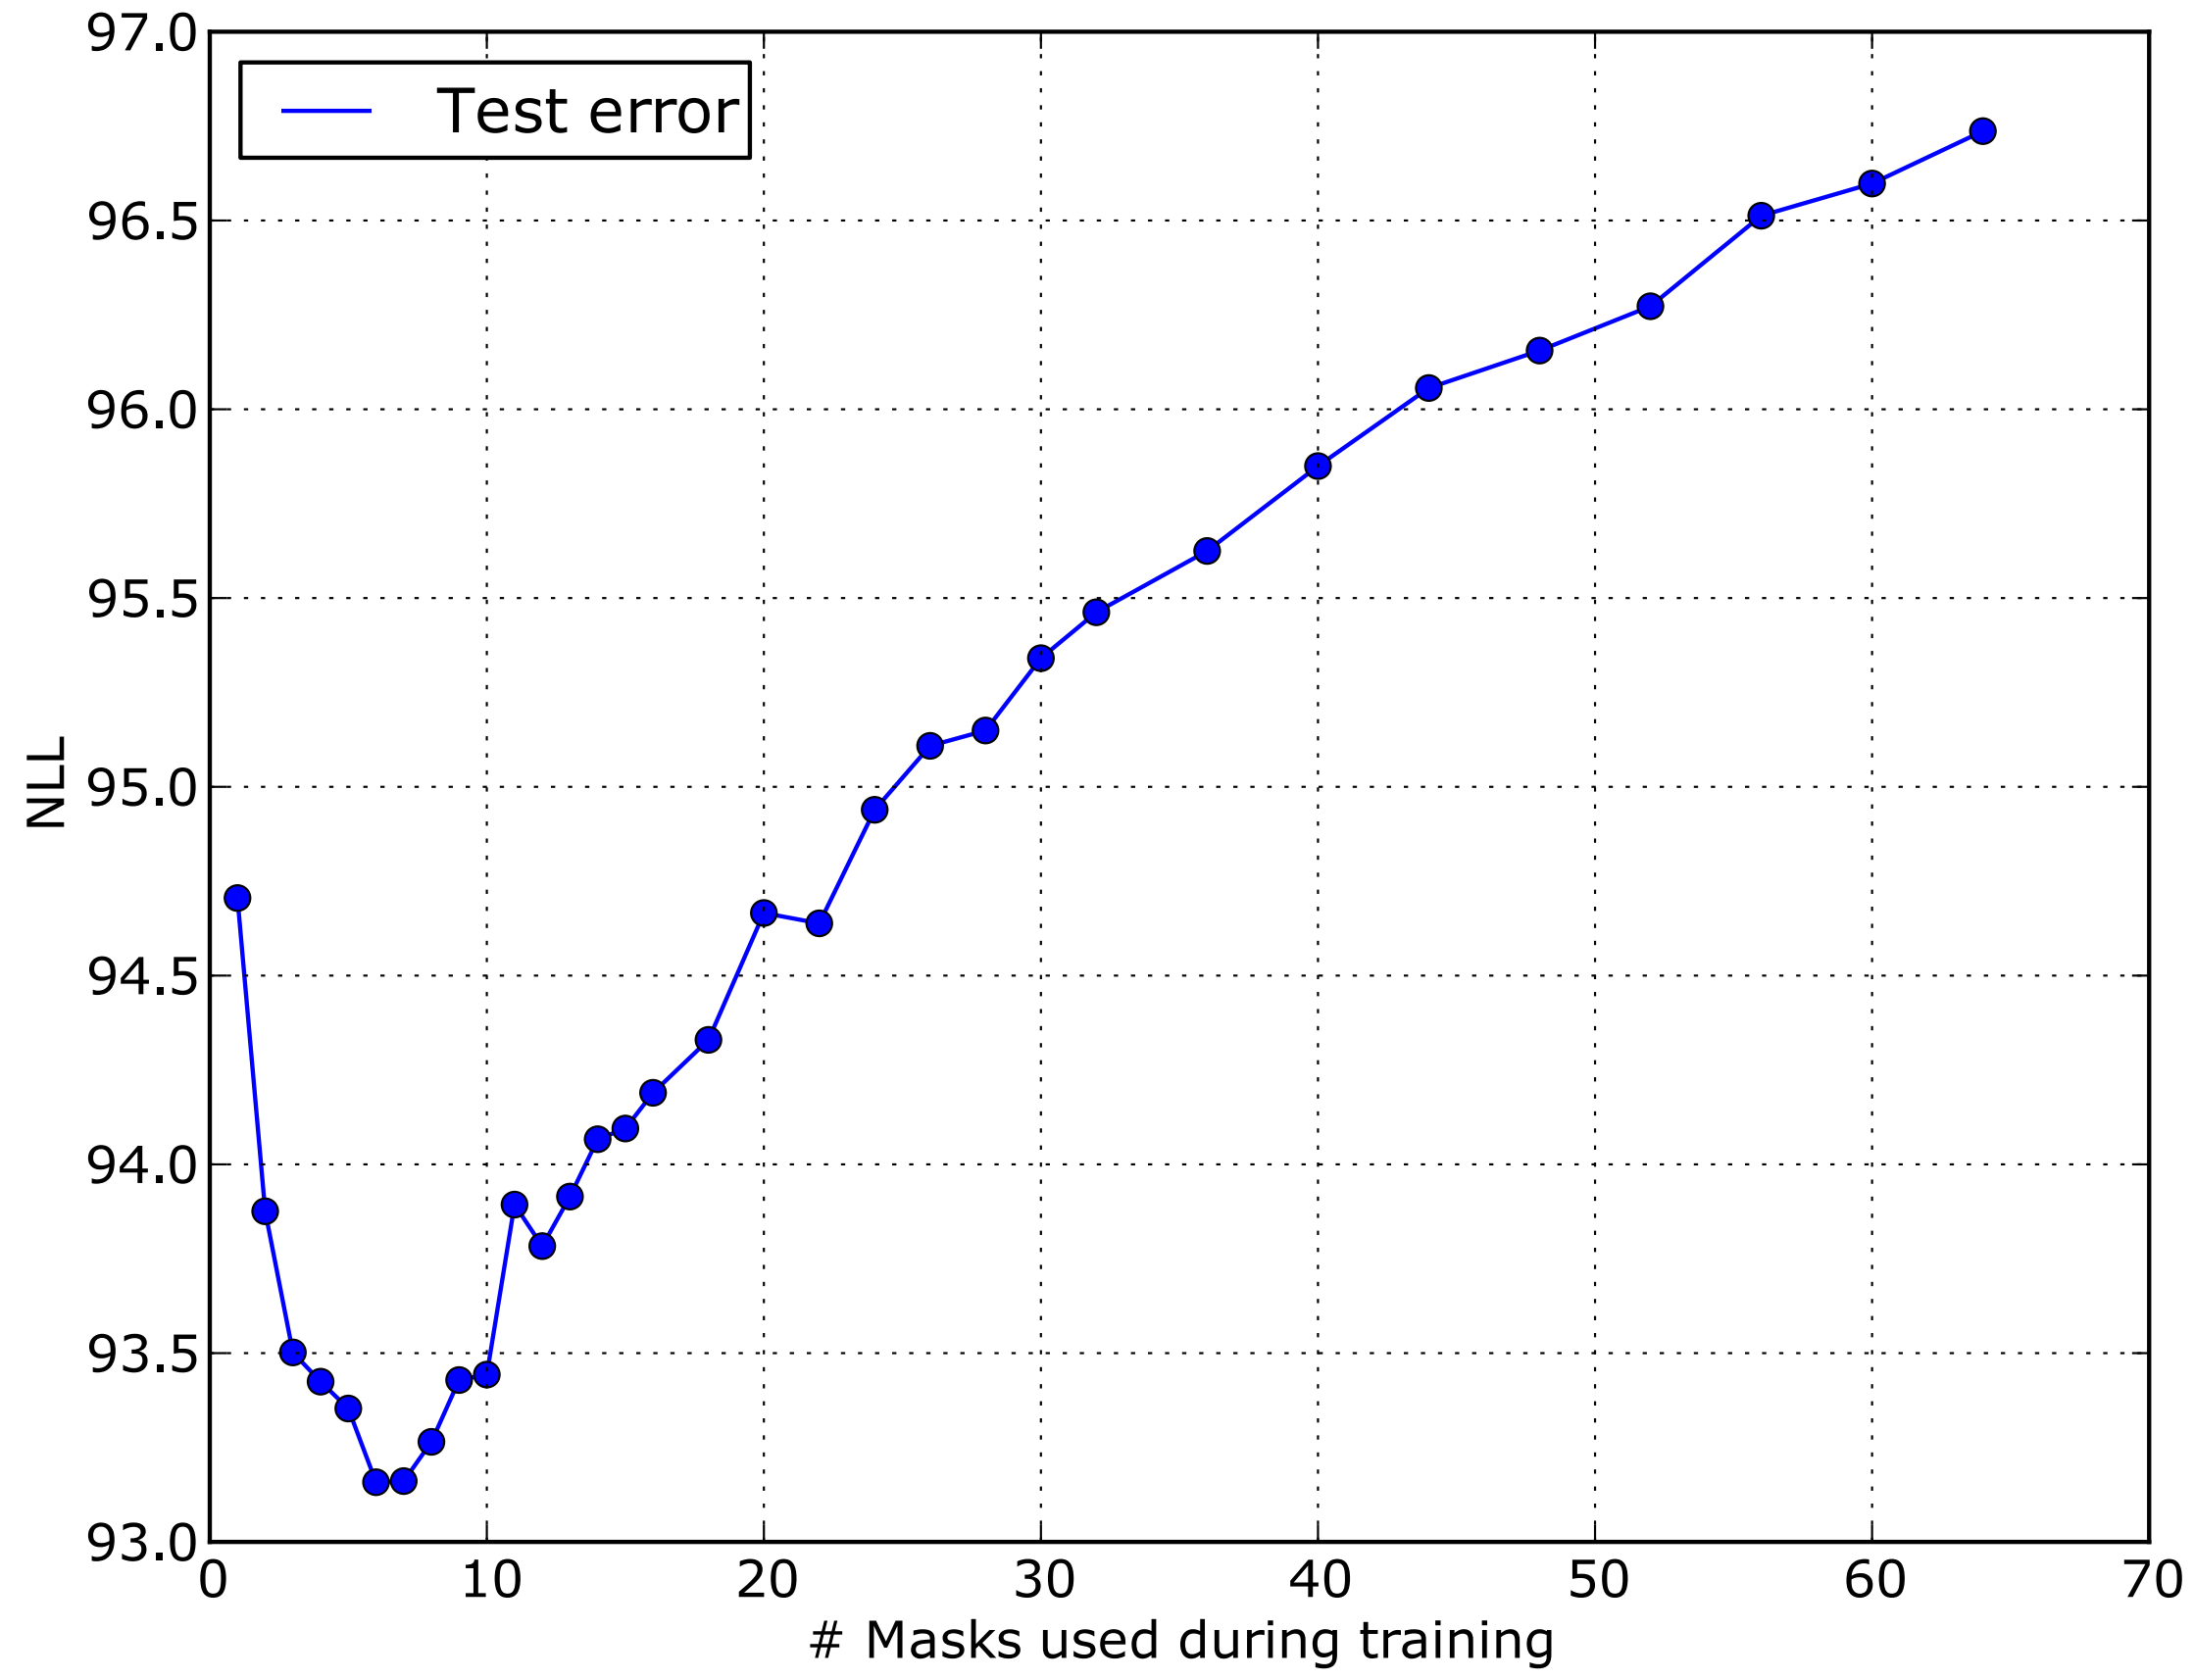
\includegraphics[width=\linewidth]{figs/made_nmasks}
		\end{figure}
	\end{minipage}%
	\begin{minipage}[t]{0.41\columnwidth}
		\begin{figure}
	  		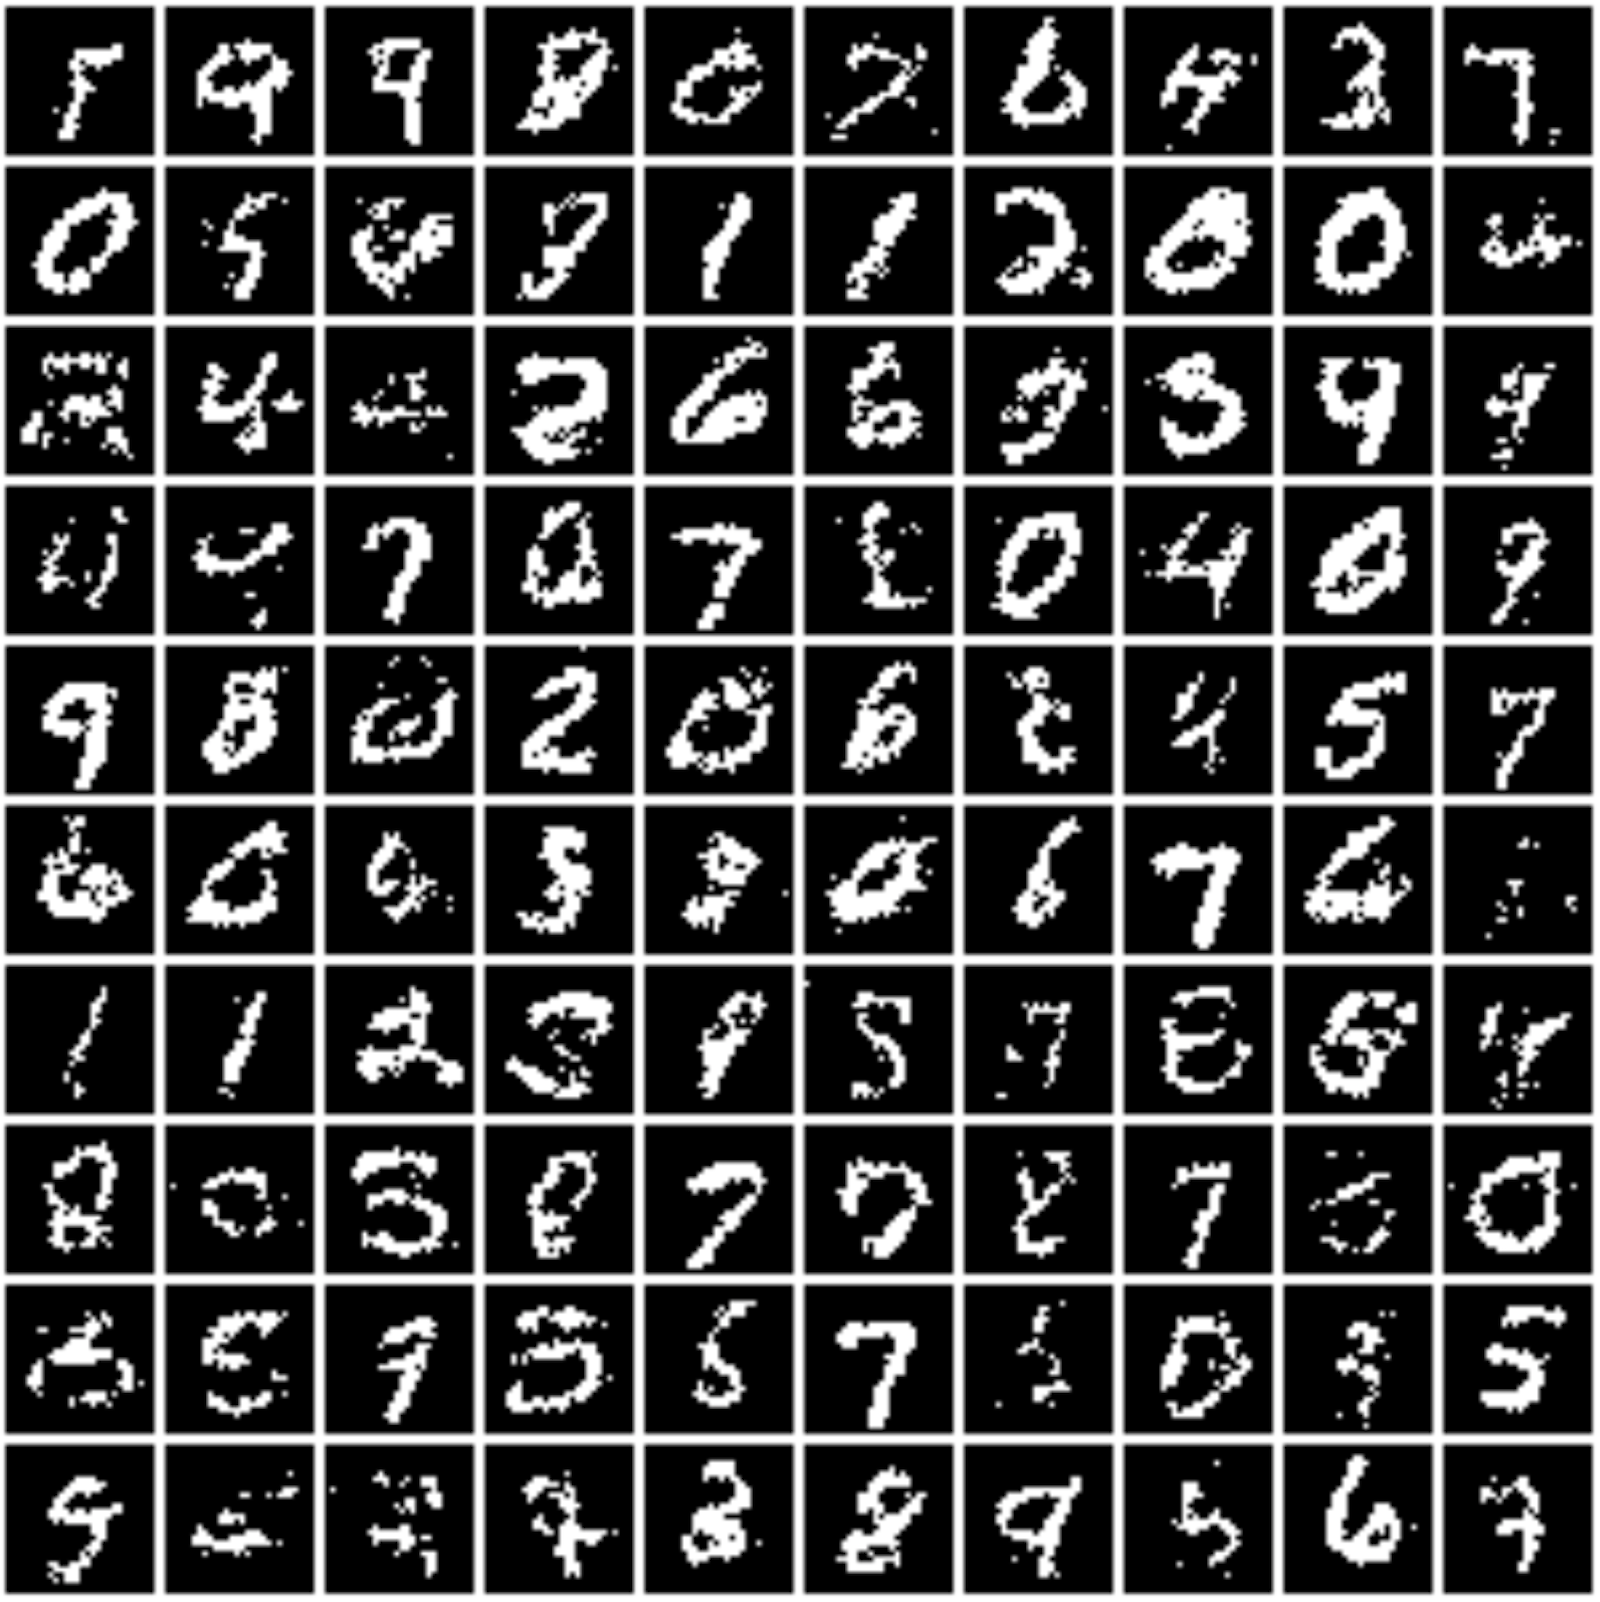
\includegraphics[width=\linewidth]{figs/made_results}
		\end{figure}
	\end{minipage}
	\myfootnotewithlink{https://arxiv.org/abs/1502.03509}{Germain M. et al. Made: Masked autoencoder for distribution estimation, 2015}
\end{frame}
%=======
\subsection{GatedPixelCNN}
%=======
\begin{frame}{GatedPixelCNN (2016)}
\begin{figure}
	\centering
	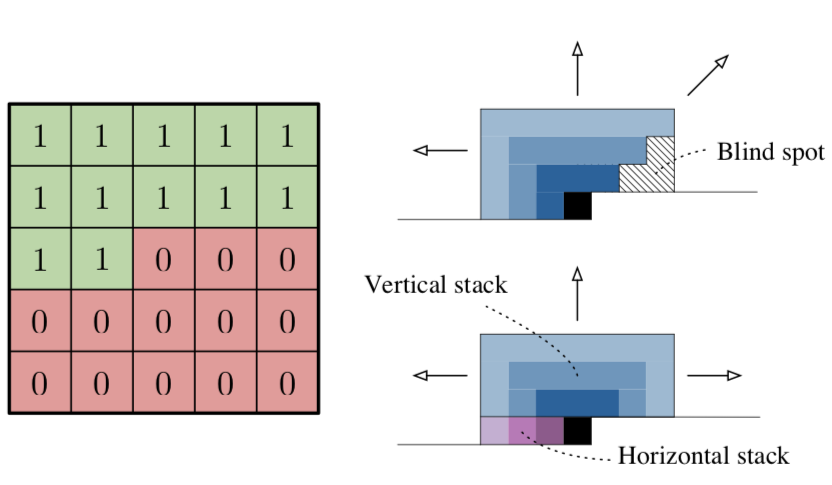
\includegraphics[width=0.5\linewidth]{figs/gatedpixelcnn.png}
	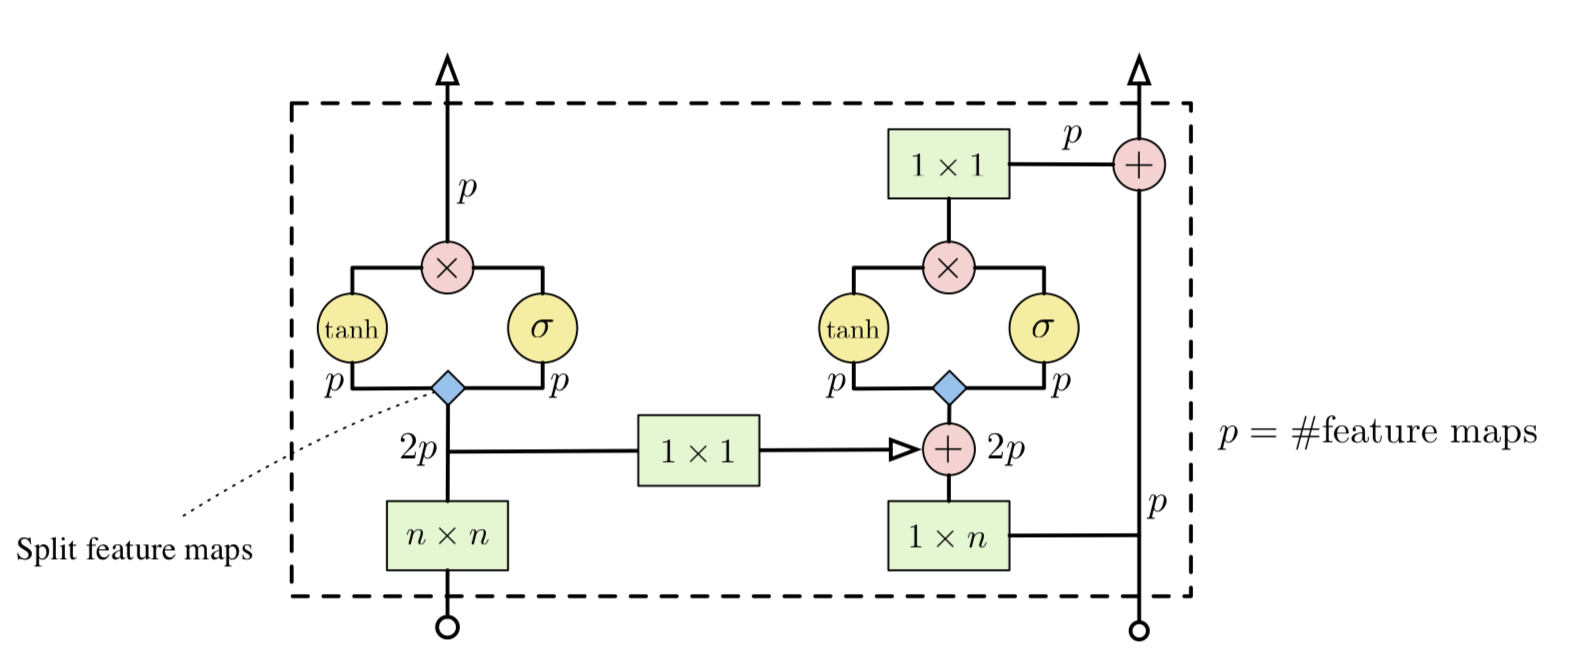
\includegraphics[width=0.5\linewidth]{figs/gated_block.png}
\end{figure}
\vfill
\hrule\medskip
{\scriptsize Van den Oord A. et al. Conditional image generation with pixelcnn decoders \href{https://arxiv.org/pdf/1606.05328.pdf}{https://arxiv.org/pdf/1606.05328.pdf}}
\end{frame}
%=======
\begin{frame}{GatedPixelCNN (2016)}
\begin{minipage}[t]{0.5\columnwidth}
	\begin{figure}[h]
		\centering
		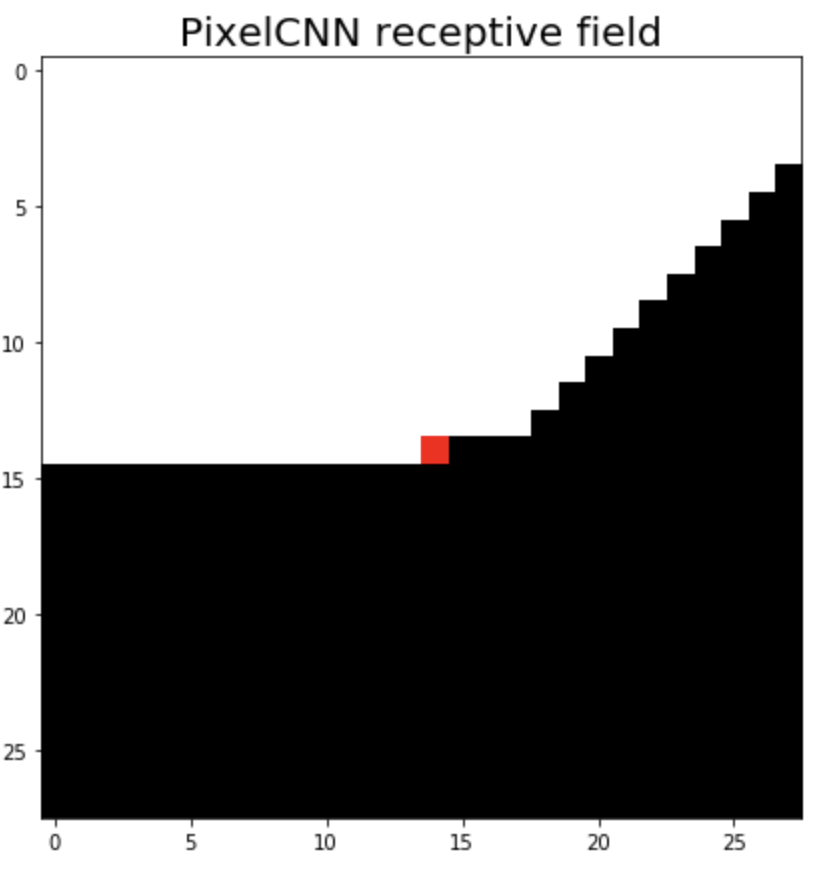
\includegraphics[width=0.9\linewidth]{figs/pixelcnn_receptive_field.png}
	\end{figure}
\end{minipage}%
\begin{minipage}[t]{0.5\columnwidth}
	\begin{figure}[h]
		\centering
		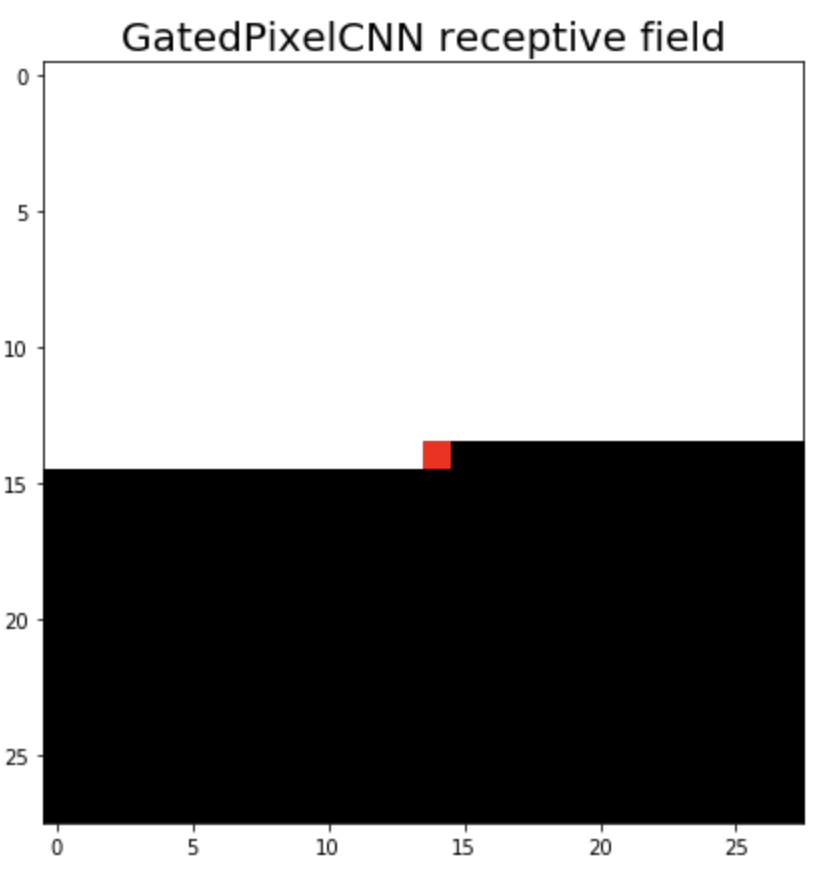
\includegraphics[width=0.9\linewidth]{figs/gatedpixelcnn_receptive_field.png}
	\end{figure}
\end{minipage}
\vfill
\hrule\medskip
{\scriptsize Van den Oord A. et al. Conditional image generation with pixelcnn decoders \href{https://arxiv.org/pdf/1606.05328.pdf}{https://arxiv.org/pdf/1606.05328.pdf}}
\end{frame}
%=======
\begin{frame}{Extensions}
\begin{itemize}
	\item \textbf{PixelCNN++}: \textit{Improving the PixelCNN with Discretized Logistic Mixture Likelihood and Other Modifications} \\
	\href{https://arxiv.org/pdf/1701.05517.pdf}{https://arxiv.org/pdf/1701.05517.pdf} \\
	(mixture of logistics instead of softmax);
	\item \textbf{PixelSNAIL}: \textit{An Improved Autoregressive Generative Model} \\
	\href{https://arxiv.org/pdf/1712.09763.pdf}{https://arxiv.org/pdf/1712.09763.pdf} \\
	(self-attention to learn optimal autoregression ordering).
\end{itemize}
\end{frame}
%=======
\section{ELBO gradient, Log derivative trick}
%=======
\begin{frame}{ELBO gradient (E-step, $\nabla_{\bphi} \mathcal{L}(\bphi, \btheta)$)}
\vspace{-0.3cm}
\[
	\mathcal{L} (\bphi, \btheta)  = \mathbb{E}_{q} \log p(\bX | \bZ, \btheta) - KL (q(\bZ| \bX, \phi) || p(\bZ)) \rightarrow \max_{\bphi, \btheta}.
\]
	Difference from M-step: density function $q(\bz| \bx, \bphi)$ depends on the parameters $\bphi$, it is impossible to use Monte-Carlo estimation:
	\[
		\nabla_{\bphi} \mathcal{L} (\bphi, \btheta) = \int \nabla_{\bphi} q(\bZ| \bX, \bphi) \log p(\bX |\bZ, \btheta) d\bZ - \nabla_{\bphi} KL
	\]
	
	\begin{block}{Log-derivative trick}
	    \[
	    \nabla_\xi q(\eta| \xi) = q(\eta | \xi) \left( \frac{\nabla_\xi q(\eta | \xi)}{q(\eta| \xi)} \right) = q(\eta | \xi) \nabla_\xi \log q(\eta| \xi).
	    \]
	\end{block}
	\[
		\nabla_{\bphi} q(\bZ| \bX, \bphi) = q(\bZ| \bX, \bphi) \nabla_{\bphi} \log q(\bZ| \bX, \bphi).
	\]
\end{frame}
%=======
\begin{frame}{ELBO gradient (E-step, $\nabla_{\bphi} \mathcal{L}(\bphi, \btheta)$)}

	\begin{multline*}
		\nabla_{\bphi} \mathcal{L} (\bphi, \btheta) = \int \nabla_{\bphi} q(\bZ| \bX, \bphi) \log p(\bX |\bZ, \btheta) d\bZ  - \nabla_{\bphi} KL = \\ 
		=  \int q(\bZ| \bX, \bphi) \bigl[  \nabla_{\bphi} \log q(\bZ| \bX, \bphi) \log p(\bX |\bZ, \btheta) \bigr] d\bZ - \nabla_{\bphi} KL
	\end{multline*}
	After applying log-reparametrization trick, we are able to use Monte-Carlo estimation:
	\[
		\nabla_{\bphi} \mathcal{L} (\bphi, \btheta) \approx n \nabla_{\bphi} \log q(\bz_i^*| \bx_i, \bphi) \log p(\bx_i |\bz_i^*, \btheta) - \nabla_{\bphi} KL,
	\]
	\[
		\bz_i^* \sim q(\bz_i| \bx_i, \bphi).
	\]
	\vspace{-0.2cm}
	\begin{block}{Problem} 
	Unstable solution with huge variance.
	\end{block}
	\begin{block}{Solution}
	    Reparametrization trick
	\end{block}
\end{frame}
%=======
\begin{frame}{Variational Autoencoder}
	Generated images for latent objects $\bz$ sampled from prior $\mathcal{N}(0, \mathbf{I})$
	\begin{figure}[h]
		\centering
		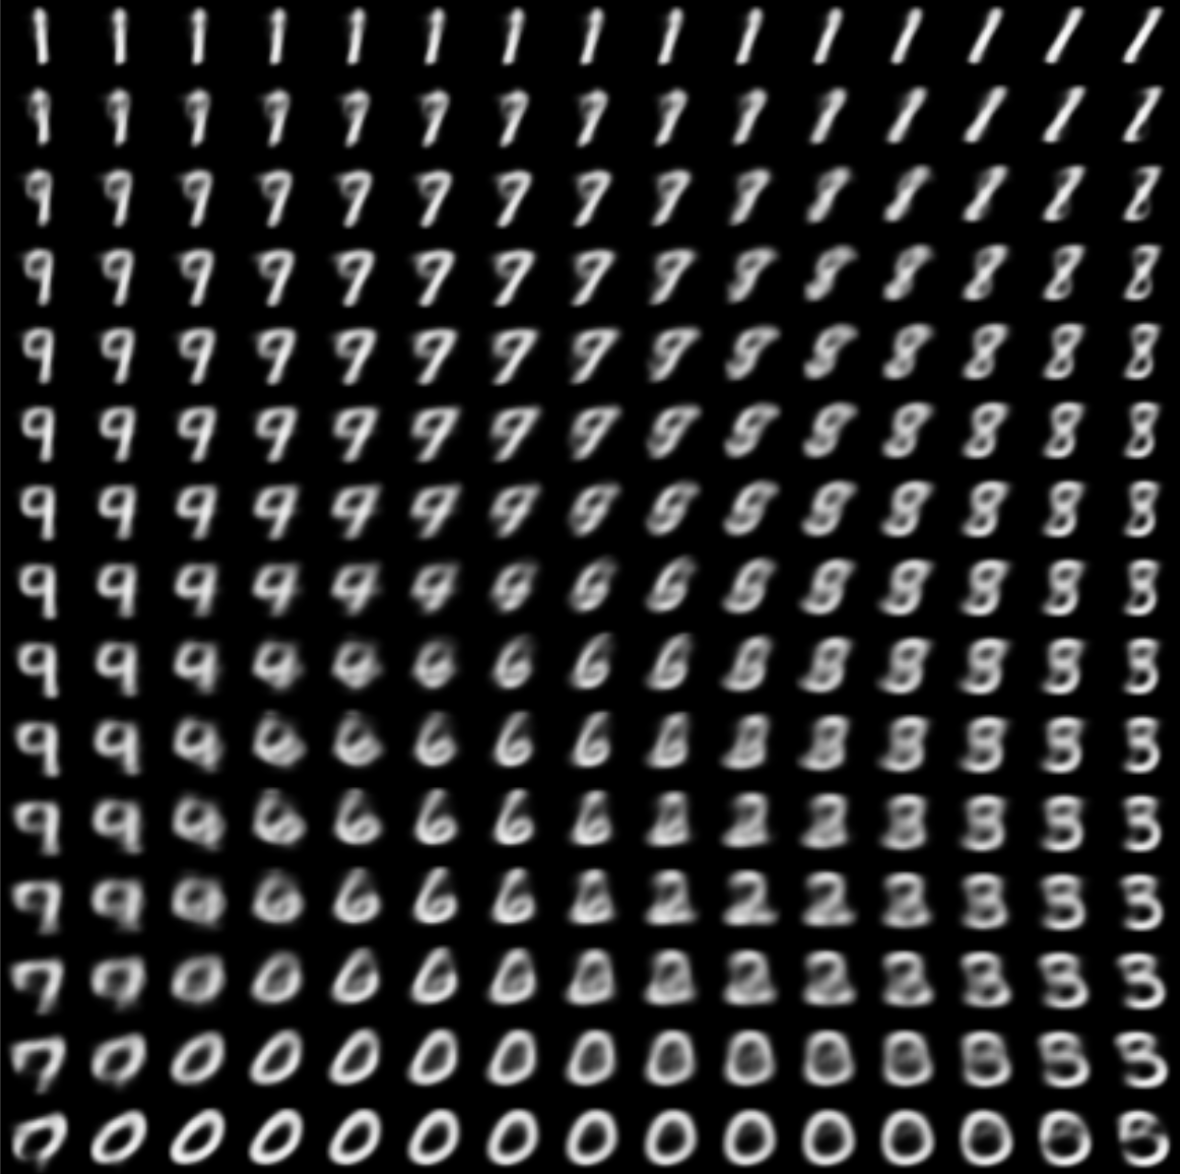
\includegraphics[width=.5\linewidth]{figs/vae_0.png}
	\end{figure}
	\myfootnotewithlink{https://habr.com/ru/post/331664}{image credit: https://habr.com/ru/post/331664}
\end{frame}
%=======
\section{Mean field approximation}
%=======
\begin{frame}{Bayesian framework}
	\begin{block}{Bayes theorem}
		\[
			p(\bt | \bx) = \frac{p(\bx | \bt) p(\bt)}{p(\bx)} = \frac{p(\bx | \bt) p(\bt)}{\int p(\bx | \bt) p(\bt) d \bt} 
		\]
		\begin{itemize}
			\item $\bx$ -- observed variables, $\bt$ -- unobserved variables (latent variables/parameters);
			\item $p(\bx | \bt)$ -- likelihood;
			\item $p(\bx) = \int p(\bx | \bt) p(\bt) d \bt$ -- evidence;
			\item $p(\bt)$ -- prior distribution, $p(\bt | \bx)$ -- posterior distribution.
		\end{itemize}
	\end{block}
	\begin{block}{Meaning}
		We have unobserved variables $\bt$ and some prior knowledge about them $p(\bt)$. Then, the data $\bx$ has been observed. 
		Posterior distribution $p(\bt | \bx)$ summarizes the knowledge after the observations.
	\end{block}
\end{frame}
%=======
\begin{frame}{Variational Lower Bound}
    We have set of objects $\bX = \{\bx_i\}_{i=1}^n$. 
    The goal is to perform Bayesian inference on the unobserved variables $\bT = \{\bt_i\}_{i=1}^n$.
    \begin{block}{Evidence Lower Bound (ELBO)}
    \vspace{-0.3cm}
        \begin{multline*}
    		\log p(\bX) 
    		= \log \frac{p(\bX, \bT)}{p(\bT|\bX)} = \\ 
    		= \int q(\bT) \log \frac{p(\bX, \bT)}{p(\bT|\bX)}d\bT
    		= \int q(\bT) \log \frac{p(\bX, \bT) q(\bT)}{p(\bT|\bX) q(\bT)} d\bT = \\
    		= \int q(\bT) \log \frac{p(\bX, \bT)}{q(\bT)}d\bT + \int q(\bT) \log \frac{q(\bT)}{p(\bT|\bX)}d\bT = \\ 
    		= \mathcal{L} (q) + KL(q(\bT) || p(\bT|\bX)) \geq \mathcal{L} (q).
    	\end{multline*}
        \vspace{-0.3cm}
    \end{block}
	We would like to maximize lower bound $\mathcal{L}(q)$.
\end{frame}
%=======
\begin{frame}{Mean field approximation}
    \begin{block}{Independence assumption}
    \vspace{-0.3cm}
    \[
    q(\bT) = \prod_{i=1}^k q_i(\bT_i), \quad \bT = [\bT_1, \dots, \bT_k], \, \bT_j = \{ \bt_{ij}\}_{i=1}^n, \, \bt_i = \{ \bT_{ij}\}_{j=1}^k.
    \]
    \vspace{-0.3cm}
    \end{block}
    \begin{block}{Block coordinate optimization of ELBO for $q_j(\bT_j)$}
  
    {\footnotesize
    \vspace{-0.3cm}
        \begin{multline*}
    		\mathcal{L} (q)
    		= \int q(\bT) \log \frac{p(\bX, \bT)}{q(\bT)}d\bT
    		= \int \left[\prod_{i=1}^k q_i(\bT_i) \right] \log \frac{p(\bX, \bT)}{\left[\prod_{i=1}^k q_i(\bT_i) \right]}  \prod_{i=1}^k d \bT_i = \\
    		= \int \left[ \prod_{i=1}^k q_i \right] \log p(\bX, \bT) \prod_{i=1}^k d \bT_i  
    		- \sum_{i=1}^k \int \left[ \prod_{j=1}^k q_j \right] \log q_i \prod_{j=1}^k d \bT_j = \\
    		= \int q_j \left[\int  \log p(\bX, \bT) \prod_{i \neq j} q_i d \bT_i \right] d \bT_j - \\
    		- \int q_j \log q_j d\bT_j + \text{const}(q_j) \rightarrow \max_{q_j}
    	\end{multline*}
        \vspace{-0.3cm}}
    \end{block}
\end{frame}
%=======
\begin{frame}{Mean field approximation}
	\footnotesize
	\begin{block}{Block coordinate optimization of ELBO for $q_j(\bT_j)$}
		\vspace{-0.4cm}
	    \begin{multline*}
			\mathcal{L} (q) 
			= \int q_j \left[\int \log p(\bX, \bT) \prod_{i \neq j} q_i d \bT_i \right] d \bT_j
			- \int q_j \log q_j  d\bT_j + \text{const}(q_j) = \\
			= \int q_j \log \hat{p}(\bX, \bT_j) d \bT_j 
			- \int q_j \log q_j d\bT_j + \text{const}(q_j) \rightarrow \max_{q_j}.
		\end{multline*}
		Here we introduce
		\[
		   \log \hat{p}(\bX, \bT_j) = \int \log p(\bX, \bT) \prod_{i \neq j} q_i d \bT_i = \mathbb{E}_{i \neq j} \log p(\bX, \bT) + \text{const}(q_j)
		\]
	    \end{block}
	    \vspace{-0.3cm}
	    \begin{block}{Final ELBO derivation for $q_j(\bT_j)$}
	    	\vspace{-0.5cm}
			\begin{multline*}
	    		\mathcal{L} (q)
	    		= \int q_j (\bT_j) \log \hat{p}(\bX, \bT_j) d \bT_j - \int q_j(\bT_j) \log q_j(\bT_j) d\bT_j + \text{const}(q_j) = \\
	    		 \int q_j (\bT_j) \log \frac{\hat{p}(\bX, \bT_j)}{q_j(\bT_j)} d\bT_j + \text{const}(q_j) = \\
	    		= - KL (q_j(\bT_j) || \hat{p}(\bX, \bT_j)) + \text{const}(q_j) \rightarrow \max_{q_j}.
	    	\end{multline*}
	    \end{block}
\end{frame}
%=======    
\begin{frame}{Mean field approximation}   
	 \begin{block}{Independence assumption}
		\vspace{-0.3cm}
		\[
		q(\bT) = \prod_{i=1}^k q_i(\bT_i), \quad \bT = [\bT_1, \dots, \bT_k], \quad \bT_j = \{ \bt_{ij}\}_{i=1}^n.
		\]
		\vspace{-0.3cm}
	\end{block}
	\begin{block}{ELBO}
	    \[
			\mathcal{L} (q) = - KL (q_j(\bT_j) || \hat{p}(\bX, \bT_j))  + \text{const}(q_j) \rightarrow \max_{q_j}.
	    \]
	    \vspace{-0.3cm}
	\end{block}
	 \begin{block}{Solution}
	 	\vspace{-0.3cm}
		 \[
		    q_j(\bT_j) = \text{const} \cdot \hat{p}(\bX, \bT_j)
		 \]
		 \[
		 	\log \hat{p}(\bX, \bT_j) = \mathbb{E}_{i \neq j} \log p(\bX, \bT) + \text{const}
		 \]
		 \[
		     \log q_j(\bT_j) = \mathbb{E}_{i \neq j} \log p(\bX, \bT) + \text{const}
		 \]
		 \vspace{-0.3cm}
	 \end{block}
\end{frame}
%=======
\begin{frame}{Mean field approximation}
	\begin{block}{ELBO}
		\[
			\mathcal{L} (q) = - KL (q_j(\bT_j) || \hat{p}(\bX, \bT_j))  + \text{const}(q_j) \rightarrow \max_{q_j}.
		\]
		\vspace{-0.3cm}
	\end{block}
	\begin{block}{Solution}
		\vspace{-0.3cm}
		\[
			\log q_j(\bT_j) = \mathbb{E}_{i \neq j} \log p(\bX, \bT) + \text{const}
		\]
		\vspace{-0.3cm}
	\end{block}
	Assumptions: 
	\begin{itemize}
		\item $\bT = [\bT_1, \bT_2] = [\bZ, \btheta]$, $q(\bT) = q(\bT_1) \cdot q(\bT_2) = q(\bZ) \cdot q(\btheta)$.
		\item restrict a class of probability distributions for $\btheta$ to Dirac delta functions:
		\[
			q_2 = q(\bT_2) = q(\btheta) = \delta(\btheta - \btheta^*).
		\]
		
		Under the restrictions the exact solution for $q_2$ is not reached (KL can be greater than 0).
	\end{itemize}
\end{frame}
%=======
\begin{frame}{Mean field approximation}
	\begin{block}{General solution}
		\vspace{-0.3cm}
		\[
		\log q_j(\bT_j) = \mathbb{E}_{i \neq j} \log p(\bX, \bT) + \text{const}
		\]
		\vspace{-0.3cm}
	\end{block}
	\begin{block}{Solution for $q_1 = q(\bZ)$}
		\vspace{-0.3cm}
		\begin{multline*}
			\log q(\bZ) = \int q(\btheta) \log p(\bX, \bZ,  \btheta) d\btheta + \text{const} = \\
			= \int \delta(\btheta - \btheta^*) \log p(\bX, \bZ,  \btheta) d\btheta + \text{const} = \\
			= \log p (\bZ | \bX, \btheta^*) +  \text{const}.
		\end{multline*}
	\end{block}
	\vspace{-0.3cm}
	\begin{block}{EM-algorithm (E-step)}
		\vspace{-0.3cm}
	\[
		q(\bZ) = \argmax_q \mathcal{L} (q, \btheta^*) = \argmin_q KL(q || p) = p(\bZ| \bX, \btheta^*).
	\]
	\end{block}
\end{frame}
%=======
\begin{frame}{Mean field approximation}
	\begin{block}{ELBO}
		\[
			\mathcal{L} (q) = - KL (q_j(\bT_j) || \hat{p}(\bX, \bT_j))  + \text{const}(q_j) \rightarrow \max_{q_j}.
		\]
	\vspace{-0.3cm}
	\end{block}
	\begin{block}{ELBO maximization w.r.t. $q_2 = q(\btheta) = \delta(\btheta - \btheta^*)$}
		\vspace{-0.3cm}
		\begin{align*}
			\mathcal{L} (q_1, q_2) &= - KL (q(\btheta) || \hat{p}(\bX, \btheta))  + \text{const}(\btheta^*) \\ 
			&= \int q (\btheta) \log \frac{\hat{p}(\bX, \btheta)}{q(\btheta)} d\btheta + \text{const}(\btheta^*) \\
			& = \int q (\btheta) \log \hat{p}(\bX, \btheta) d\btheta  - \int q (\btheta) \log q(\btheta) d\btheta + \text{const}(\btheta^*) \\
			& = \int \delta(\btheta - \btheta^*) \log \hat{p}(\bX, \btheta) d\btheta + \text{const}(\btheta^*) \rightarrow \max_{\btheta^*}
		\end{align*}
		\vspace{-0.3cm}
	\end{block}
\end{frame}
%=======
\begin{frame}{Mean field approximation}
	
	\begin{block}{ELBO maximization w.r.t. $q_2 = q(\btheta) = \delta(\btheta - \btheta^*)$}
		\vspace{-0.3cm}
		\begin{multline*}
			\mathcal{L} (q_1, q_2) = \int \delta(\btheta - \btheta^*) \log \hat{p}(\bX, \btheta) d\btheta + \text{const}
			= \log \hat{p}(\bX, \btheta^*)  + \text{const} \\
			= \mathbb{E}_{i \neq j} \log p(\bX, \bT) + \text{const} = \mathbb{E}_{q_1} \log p(\bX, \bZ, \btheta^*) + \text{const} \\
		= \int q(\bZ) \log p(\bX, \bZ|  \btheta^*) d\bZ + \log p(\btheta^*)+ \text{const}\rightarrow \max_{\btheta^*}
	\end{multline*}
	\end{block}
	\vspace{-0.3cm}
	\begin{block}{EM-algorithm (M-step)}
		\vspace{-0.3cm}
		 \begin{align*}
		 	\mathcal{L}(q, \btheta) &= \int q(\bZ) \log \frac{p(\bX, \bZ | \btheta)}{q(\bZ)}d\bZ \\
		 	&= \int q(\bZ) \log p(\bX, \bZ | \btheta) d\bZ + \text{const} \rightarrow \max_{\btheta}
		 \end{align*}
	\end{block}
\end{frame}
%=======
\begin{frame}{Mean field approximation}
    \begin{block}{Solution}
    \[
        \log q_j(\bT_j) = \mathbb{E}_{i \neq j} \log p(\bX, \bT) + \text{const}
    \]
    \end{block}

	\begin{block}{EM algorithm (special case)}
	\begin{itemize}
		\item Initialize $\btheta^*$;
		\item E-step
		\[
			q(\bZ) = \argmax_q \mathcal{L} (q, \btheta^*) = \argmin_q KL(q || p) =
			 p(\bZ| \bX, \btheta^*);
		\]
		\item M-step
		\[
			\btheta^* = \argmax_{\btheta} \mathcal{L} (q, \btheta);
		\]
		\item Repeat E-step and M-step until convergence.
	\end{itemize}
	\end{block}
\end{frame}
%=======
\section{IWAE}
%=======
\begin{frame}{IWAE}
	\begin{block}{Theorem}
		\begin{enumerate}
			\item $\log p(\bx | \btheta) \geq \mathcal{L}_K (q, \btheta) \geq \mathcal{L}_M (q, \btheta), \quad \text{for } K \geq M$;
			\item $\log p(\bx | \btheta) = \lim_{K \rightarrow \infty} \mathcal{L}_K (q, \btheta)$ if $\frac{p(\bx, \bz | \btheta)}{q(\bz | \bx)}$ is bounded.
		\end{enumerate}
		\vspace{-0.2cm}
	\end{block}
	\begin{block}{Proof of 1.}
		{ \footnotesize
			\vspace{-0.6cm}
			\begin{align*}
				\mathcal{L}_K (q, \btheta) &= \mathbb{E}_{\bz_1, \dots, \bz_K} \log \left( \frac{1}{K}\sum_{k=1}^K\frac{p(\bx, \bz_k | \btheta)}{q(\bz_k| \bx)} \right) = \\
				&= \mathbb{E}_{\bz_1, \dots, \bz_K} \log \mathbb{E}_{k_1, \dots, k_M} \left( \frac{1}{M}\sum_{m=1}^M\frac{p(\bx, \bz_{k_M} | \btheta)}{q(\bz_{k_m}| \bx)} \right) \geq \\
				&\geq \mathbb{E}_{\bz_1, \dots, \bz_K} \mathbb{E}_{k_1, \dots, k_m} \log \left( \frac{1}{M}\sum_{m=1}^M\frac{p(\bx, \bz_{k_m} | \btheta)}{q(\bz_{k_m}| \bx)} \right) = \\
				&= \mathbb{E}_{\bz_1, \dots, \bz_M} \log \left( \frac{1}{M}\sum_{m=1}^M\frac{p(\bx, \bz_m | \btheta)}{q(\bz_m| \bx)} \right) = \mathcal{L}_M (q, \btheta)
			\end{align*}
			\[
			\frac{a_1 + \dots + a_K}{K} = \mathbb{E}_{k_1, \dots, k_M} \frac{a_{k_1} + \dots + a_{k_M}}{M}, \quad k_1, \dots, k_M \sim U[1, K]
			\]
		}
	\end{block}
	
	\myfootnotewithlink{https://arxiv.org/abs/1509.00519}{Burda Y., Grosse R., Salakhutdinov R. Importance Weighted Autoencoders, 2015}
\end{frame}
%=======
\begin{frame}{IWAE}
	\begin{block}{Theorem}
		\begin{enumerate}
			\item $\log p(\bx | \btheta) \geq \mathcal{L}_K (q, \btheta) \geq \mathcal{L}_M (q, \btheta), \quad \text{for} K \geq M$;
			\item $\log p(\bx | \btheta) = \lim_{K \rightarrow \infty} \mathcal{L}_K (q, \btheta)$ if $\frac{p(\bx, \bz | \btheta)}{q(\bz | \bx)}$ is bounded.
		\end{enumerate}
		\vspace{-0.2cm}
	\end{block}
	\begin{block}{Proof of 2.}
		\vspace{0.2cm}
		Consider r.v. $\xi_K = \frac{1}{K}\sum_{k=1}^K \frac{p(\bx, \bz_k | \btheta)}{q(\bz_k | \bx)}$. \\
		\vspace{0.2cm}
		If summands are bounded, then (from the strong law of large numbers)
		\[
		\xi_K \xrightarrow[K \rightarrow \infty]{a.s.} \mathbb{E}_{q(\bz | \bx)} \frac{p(\bx, \bz | \btheta)}{q(\bz | \bx)} = p(\bx | \btheta).
		\]
		Hence $\mathcal{L}_K (q, \btheta) = \mathbb{E} \log \xi_K$ converges to $\log p(\bx | \btheta)$ as $K \rightarrow \infty$.
	\end{block}

	\myfootnotewithlink{https://arxiv.org/abs/1509.00519}{Burda Y., Grosse R., Salakhutdinov R. Importance Weighted Autoencoders, 2015}
\end{frame}
%=======
\begin{frame}{Importance Weighted Autoencoders (IWAE)}
	\begin{block}{Theorem}
		\begin{enumerate}
			\item $\log p(\bx | \btheta) \geq \mathcal{L}_K (q, \btheta) \geq \mathcal{L}_M (q, \btheta), \quad \text{for } K \geq M$;
			\item $\log p(\bx | \btheta) = \lim_{K \rightarrow \infty} \mathcal{L}_K (q, \btheta)$ if $\frac{p(\bx, \bz | \btheta)}{q(\bz | \bx, \bphi)}$ is bounded.
		\end{enumerate}
		\vspace{-0.2cm}
	\end{block}
	If $K > 1$ the bound could be tighter.
	\begin{align*}
		\mathcal{L} (q, \btheta) &= \mathbb{E}_{q(\bz | \bx, \bphi)} \log \frac{p(\bx, \bz | \btheta)}{q(\bz| \bx, \bphi)}; \\
		\mathcal{L}_K (q, \btheta) &= \mathbb{E}_{\bz_1, \dots, \bz_K \sim q(\bz | \bx, \bphi)} \log \left( \frac{1}{K}\sum_{k=1}^K\frac{p(\bx, \bz_k | \btheta)}{q(\bz_k| \bx, \bphi)} \right).
	\end{align*}
	\vspace{-0.2cm}
	\begin{itemize}
		\item $\mathcal{L}_1(q, \btheta) = \mathcal{L}(q, \btheta)$;
		\item $\mathcal{L}_{\infty}(q, \btheta) = \log p(\bx | \btheta)$.
		\item Which $q^*(\bz | \bx, \bphi)$ gives $\mathcal{L}(q^*, \btheta) = \log p(\bx | \btheta)$? 
		\item Which $q^*(\bz | \bx, \bphi)$ gives $\mathcal{L}(q^*, \btheta) = \mathcal{L}_K(q, \btheta)$?
	\end{itemize}

	\myfootnotewithlink{https://arxiv.org/abs/1509.00519}{Burda Y., Grosse R., Salakhutdinov R. Importance Weighted Autoencoders, 2015}
\end{frame}
%=======
\begin{frame}{Importance Weighted Autoencoders (IWAE)}
	\begin{block}{Theorem}
		$\mathcal{L}(q^*, \btheta) = \mathcal{L}_K(q, \btheta)$
		for the following variational distribution
		\[
		q^*(\bz | \bx, \bphi) = \mathbb{E}_{\bz_2, \dots, \bz_K \sim q(\bz | \bx)} q_{IW}(\bz | \bx, \bz_{2:K}),
		\]
		where
		\vspace{-0.4cm}
		\[
			q_{IW}(\bz | \bx, \bz_{2:K}) = \frac{\frac{p(\bx, \bz)}{q(\bz | \bx)}}{\frac{1}{K} \sum_{k=1}^K \frac{p(\bx, \bz_k)}{q(\bz_k | \bx)}} q(\bz | \bx) = \frac{p(\bx, \bz)}{\frac{1}{K}\left( \frac{p(\bx, \bz)}{q(\bz | \bx)} + \sum_{k=2}^K \frac{p(\bx, \bz_k)}{q(\bz_k | \bx)}\right)}.
		\]
	\end{block}
	\vspace{-0.5cm}
	\begin{block}{IWAE posterior}
		\vspace{-0.3cm}
		\begin{figure}
			\centering
			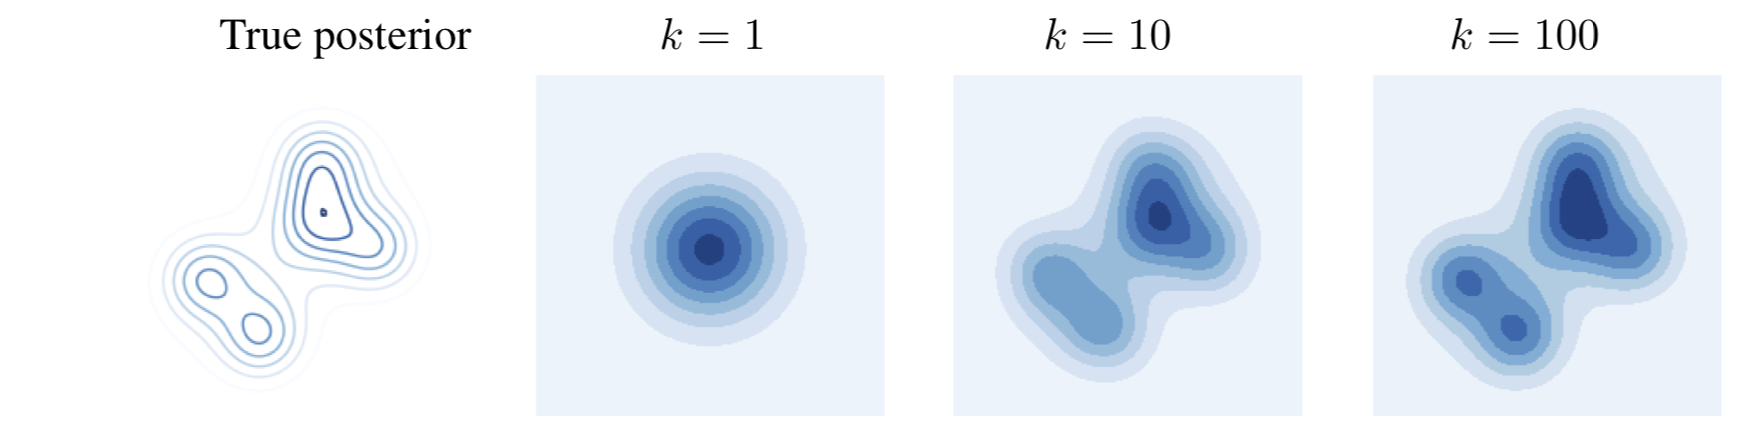
\includegraphics[width=\linewidth]{figs/IWAE_1.png}
		\end{figure}
	\end{block}

	\myfootnotewithlink{https://arxiv.org/abs/1704.02916}{Cremer C., Morris Q., Duvenaud D. Reinterpreting Importance-Weighted Autoencoders, 2017}
\end{frame}
%=======
\begin{frame}{IWAE, 2015}
How to determine whether all VAE latent variables are informative?
\[
A_{i} = \text{cov}_\bx \left( \mathbb{E}_{q(z_i | \bx)} [z_i] \right) > 0.01 \quad \Leftrightarrow \quad z_i \text{ is active}
\]
\begin{figure}
	\centering
	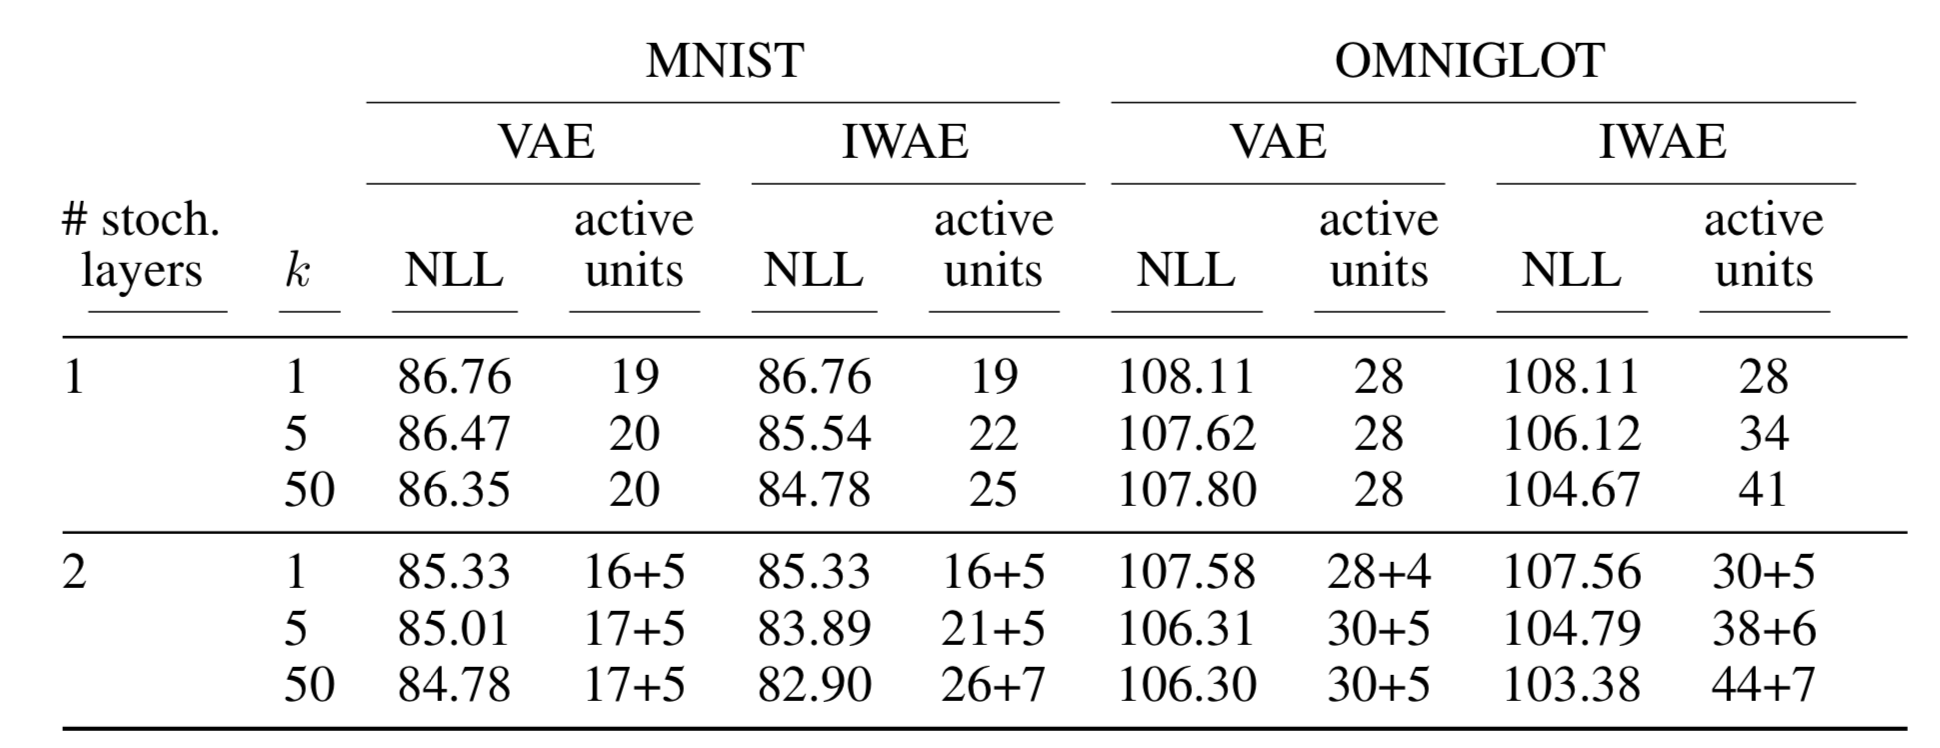
\includegraphics[width=\linewidth]{figs/IWAE_3.png}
\end{figure}
\vfill
\hrule\medskip
{\scriptsize \href{https://arxiv.org/pdf/1509.00519.pdf}{https://arxiv.org/pdf/1509.00519.pdf}}
\end{frame}
%=======
\section{PixelVAE, Hierarchical VAE}
%=======
\begin{frame}{PixelVAE, 2016}
	\begin{block}{Hierarchical VAE}
		\begin{figure}
			\centering
			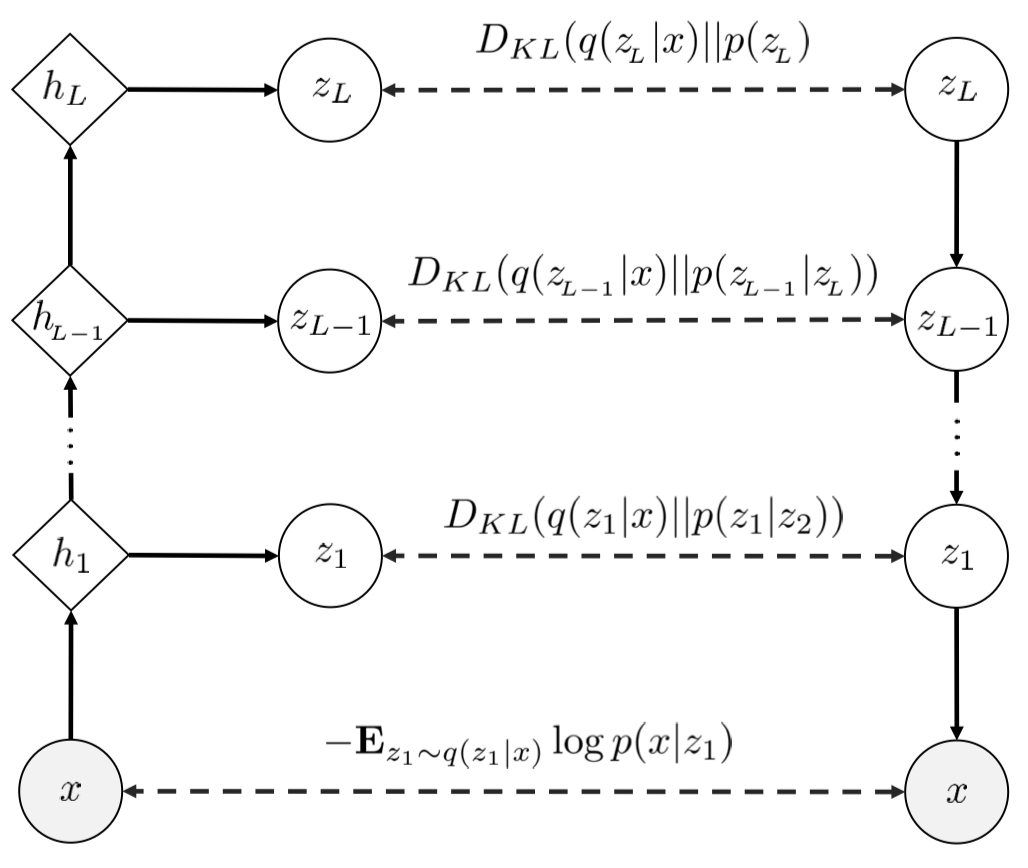
\includegraphics[width=0.7\linewidth]{figs/PixelVAE_1.png}
		\end{figure}
	\end{block}
	\vfill
	\hrule\medskip
	{\scriptsize \href{https://arxiv.org/pdf/1611.05013.pdf}{https://arxiv.org/pdf/1611.05013.pdf}}
\end{frame}
%=======
\begin{frame}{PixelVAE, 2016}
	\begin{block}{Hierarchical decomposition}
		\vspace{-1cm}
		\begin{align*}
			p(\bz_1, \dots, \bz_L) &= p(\bz_L) p(\bz_{L-1} | \bz_L) \dots p(\bz_1, \bz_2); \\
			q(\bz_1, \dots, \bz_L | \bx) &= q(\bz_1 | \bx) \dots q(\bz_L | \bx).
		\end{align*}
	\end{block}
	\vspace{-0.5cm}
	\begin{block}{ELBO}
		\vspace{-0.5cm}
		{\footnotesize
			\begin{align*}
				\mathcal{L}(q, \btheta) &= \mathbb{E}_{q(\bz_1 | \bx)} \log p(\bx | \bz_1, \btheta) - KL(q(\bz_1, \dots, \bz_L | \bx) || p(\bz_1, \dots, \bz_L)) \\
				&= \mathbb{E}_{q(\bz_1 | \bx)} \log p(\bx | \bz_1, \btheta) - \int \prod_{j=1}^L q(\bz_j | \bx) \sum_{i=1}^L \log \frac{q(\bz_i | \bx)}{p(\bz_i | \bz_{i + 1})} d \bz_1 \dots d \bz_L \\
				&= \mathbb{E}_{q(\bz_1 | \bx)} \log p(\bx | \bz_1, \btheta) - \sum_{i=1}^L \int \prod_{j=1}^L q(\bz_j | \bx) \log \frac{q(\bz_i | \bx)}{p(\bz_i | \bz_{i + 1})} d \bz_1 \dots d \bz_L \\
				&= \mathbb{E}_{q(\bz_1 | \bx)} \log p(\bx | \bz_1, \btheta) - \sum_{i=1}^L \int q(\bz_{i+1} | \bx) q(\bz_i | \bx) \log \frac{q(\bz_i | \bx)}{p(\bz_i | \bz_{i + 1})} d \bz_i d \bz_{i+1} \\
				&= \mathbb{E}_{q(\bz_1 | \bx)} \log p(\bx | \bz_1, \btheta) - \sum_{i=1}^L \mathbb{E}_{q(\bz_{i+1} | \bx)} \left[ KL (q(\bz_i | \bx) || p(\bz_i | \bz_{i + 1}))\right]
			\end{align*}
		}
	\end{block}
	\vfill
	\hrule\medskip
	{\scriptsize \href{https://arxiv.org/pdf/1611.05013.pdf}{https://arxiv.org/pdf/1611.05013.pdf}}
\end{frame}
%=======
\section{Posterior collapse}
%=======
\begin{frame}{Posterior collapse: toy example}
	Let define latent variable model in the following way:
	\[
	p(\bx | \btheta) = \int p(\bx, \bz | \btheta) d \bz = \int p(\bx | \bz, \btheta) p(\bz) d \bz 
	\]
	\begin{itemize}
		\item prior distribution $p(\bz) = \mathcal{N}(\bz| 0, \mathbf{I})$;
		\item probabilistic model $p(\bx | \bz, \btheta) = \mathcal{N}(\bx | \bmu_{\btheta}(\bz), \bsigma_{\btheta}(\bz))$ (diagonal covariance);
		\item variational posterior $q(\bz | \bx, \bphi) =  \mathcal{N}(\bx | \bmu_{\bphi}(\bx), \bsigma_{\phi}(\bx))$  (diagonal covariance).
	\end{itemize}
	
	Let data distribution is $\pi(\bx) = \mathcal{N}(\bx | \bmu, \bSigma)$. Possible cases:
	\begin{itemize}
		\item covariance matrix $\bSigma$ is diagonal (univariate case);
		\item covariance matrix $\bSigma$ is \textbf{not} diagonal (multivariate case).
	\end{itemize}
	What is the difference?
\end{frame}
%=======
\begin{frame}{Posterior collapse: toy example + VLAE}
	\begin{block}{Multivariate ($\bSigma$ is non-diagonal)}
		\vspace{-0.5cm}
		\begin{minipage}[t]{0.33\columnwidth}
			\begin{figure}[h]
				\centering
				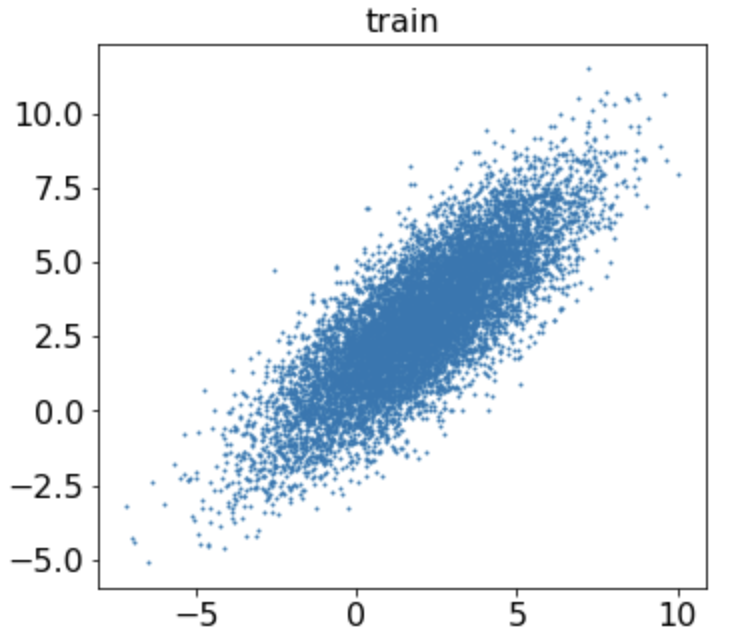
\includegraphics[width=.8\linewidth]{figs/posterior_collapse_toy_1.png}
			\end{figure}
		\end{minipage}%
		\begin{minipage}[t]{0.33\columnwidth}
			\begin{figure}[h]
				\centering
				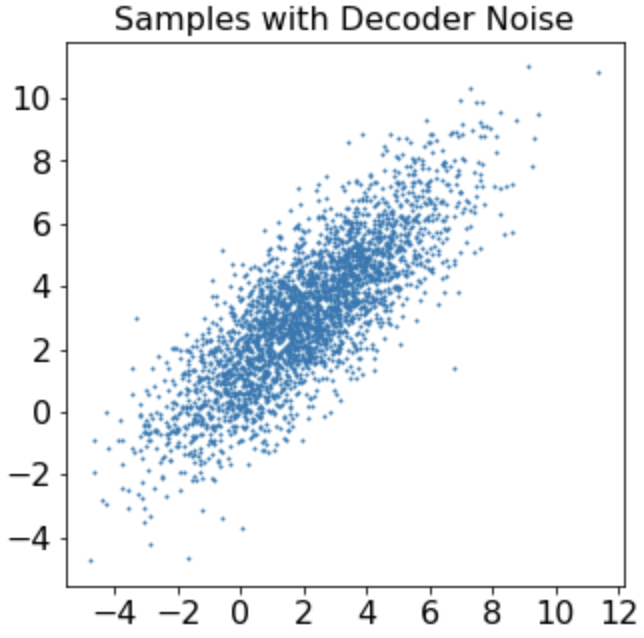
\includegraphics[width=0.75\linewidth]{figs/posterior_collapse_toy_3.png}
			\end{figure}
		\end{minipage}%
		\begin{minipage}[t]{0.33\columnwidth}
			\begin{figure}[h]
				\centering
				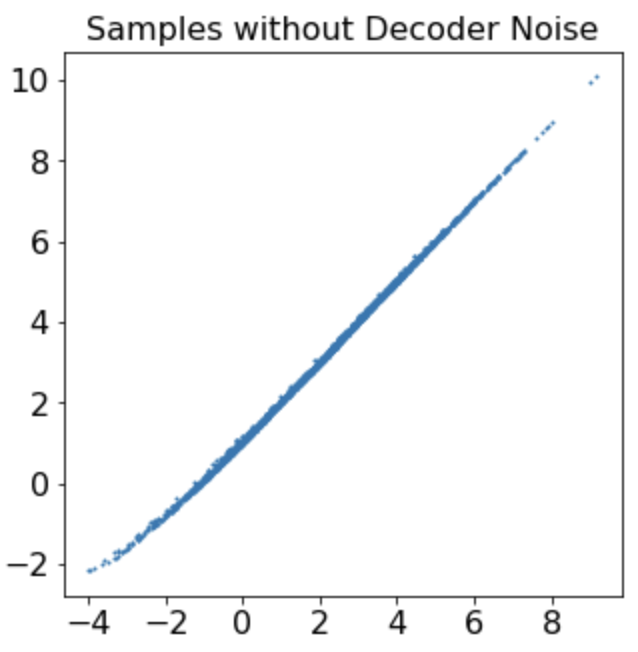
\includegraphics[width=.75\linewidth]{figs/posterior_collapse_toy_5.png}
			\end{figure}
		\end{minipage}
		The encoder uses latent variables to model data.
	\end{block}
	
	\begin{block}{Univariate ($\bSigma$ is diagonal)}
		\vspace{-0.5cm}
		\begin{minipage}[t]{0.33\columnwidth}
			\begin{figure}[h]
				\centering
				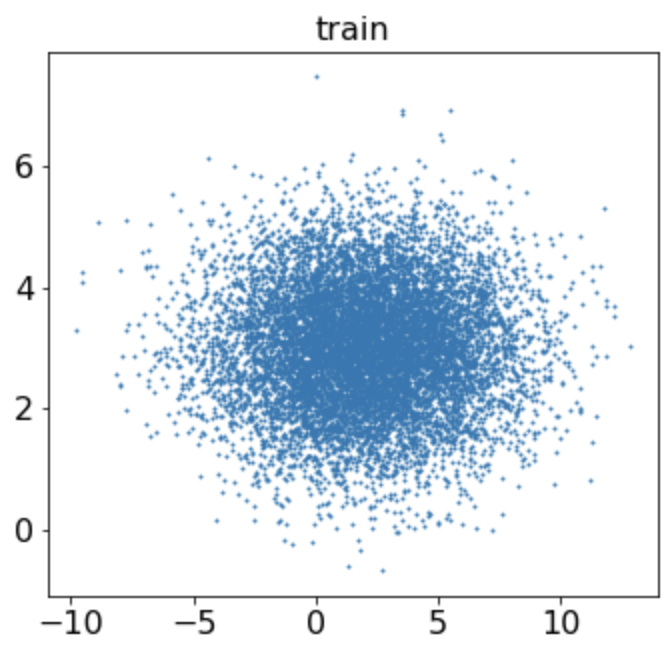
\includegraphics[width=.8\linewidth]{figs/posterior_collapse_toy_2.png}
			\end{figure}
		\end{minipage}%
		\begin{minipage}[t]{0.33\columnwidth}
			\begin{figure}[h]
				\centering
				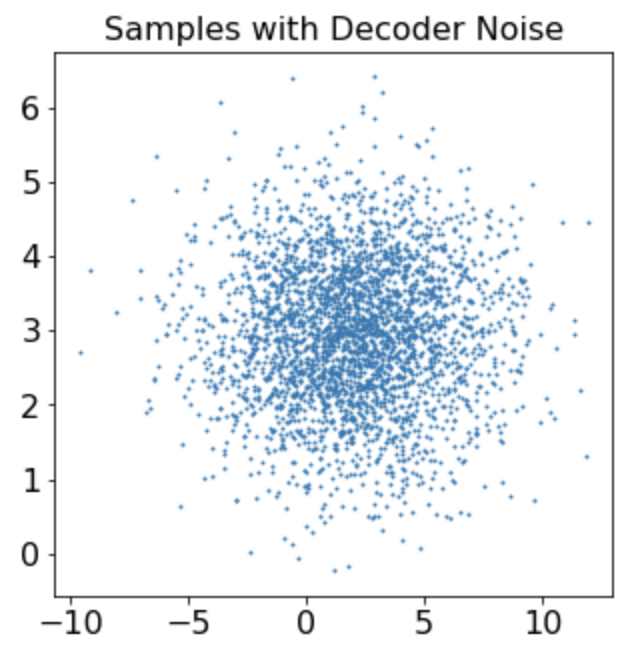
\includegraphics[width=.75\linewidth]{figs/posterior_collapse_toy_4.png}
			\end{figure}
		\end{minipage}%
		\begin{minipage}[t]{0.33\columnwidth}
			\begin{figure}[h]
				\centering
				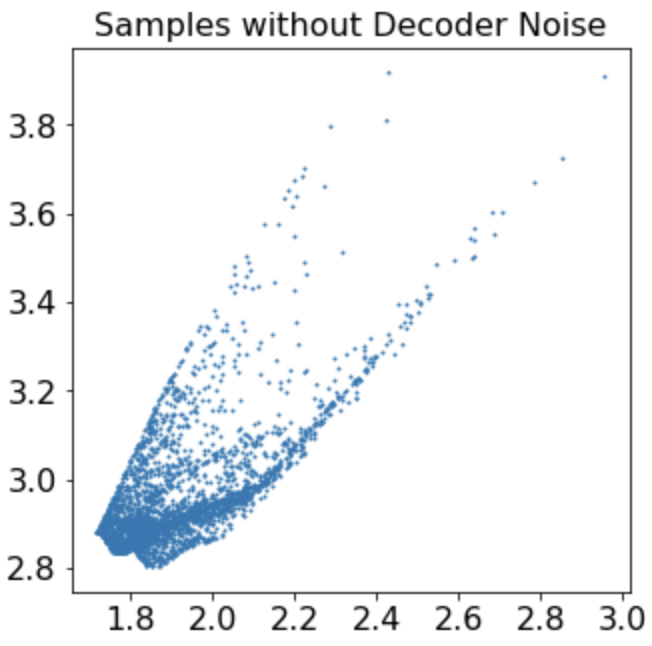
\includegraphics[width=.75\linewidth]{figs/posterior_collapse_toy_6.png}
			\end{figure}
		\end{minipage}
		Latent variables are not used, since the decoder could model the data without the encoder.
	\end{block}
\end{frame}
%=======
\begin{frame}{Variational Lossy AutoEncoder}
	\begin{block}{Lossy code via explicit information placement}
		\[
		p(\bx | \bz, \btheta) = \prod_{i=1}^m p(x_i | \bz, \bx_{\text{WindowAround}(i)}, \btheta).
		\]
		\begin{itemize}
			\item WindowAround($i$) restricts the receptive field (it forbids to represent arbitrarily complex distribution over $\bx$ without dependence on $\bz$). 
			\item Local statistics of 2D images (texture) will be modeled by a small local window.
			\item Global structural information (shapes) is long-range dependency that can only be communicated through latent code $\bz$. 
		\end{itemize}
	\end{block}
	\myfootnotewithlink{https://arxiv.org/abs/1611.02731}{Chen X. et al. Variational Lossy Autoencoder, 2016}
\end{frame}
%=======
\begin{frame}{Variational Lossy AutoEncoder}
	\begin{itemize}
		\item Can VLAE learn lossy codes that encode global statistics?
		\item Does using AF priors improves upon using IAF posteriors as predicted by theory?
		\item Does using autoregressive decoding distributions improve density estimation performance?
	\end{itemize}
	\begin{minipage}[t]{0.5\columnwidth}
		\vspace{1cm}
		MNIST
		\begin{figure}[h]
			\centering
			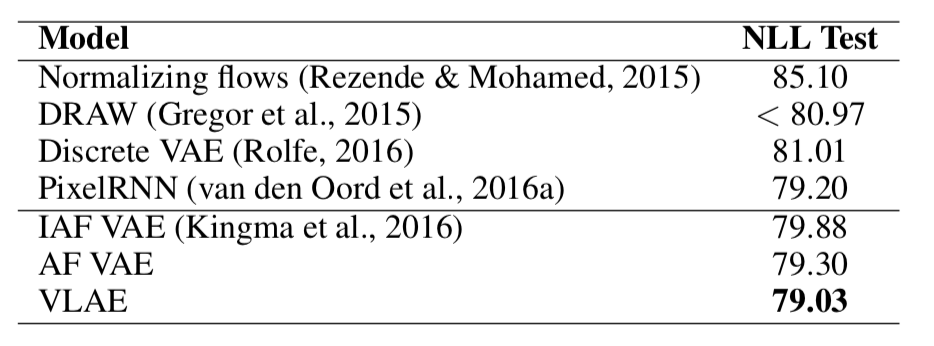
\includegraphics[width=1.\linewidth]{figs/VLAE_1.png}
		\end{figure}
	\end{minipage}%
	\begin{minipage}[t]{0.5\columnwidth}
		CIFAR10
		\begin{figure}[h]
			\centering
			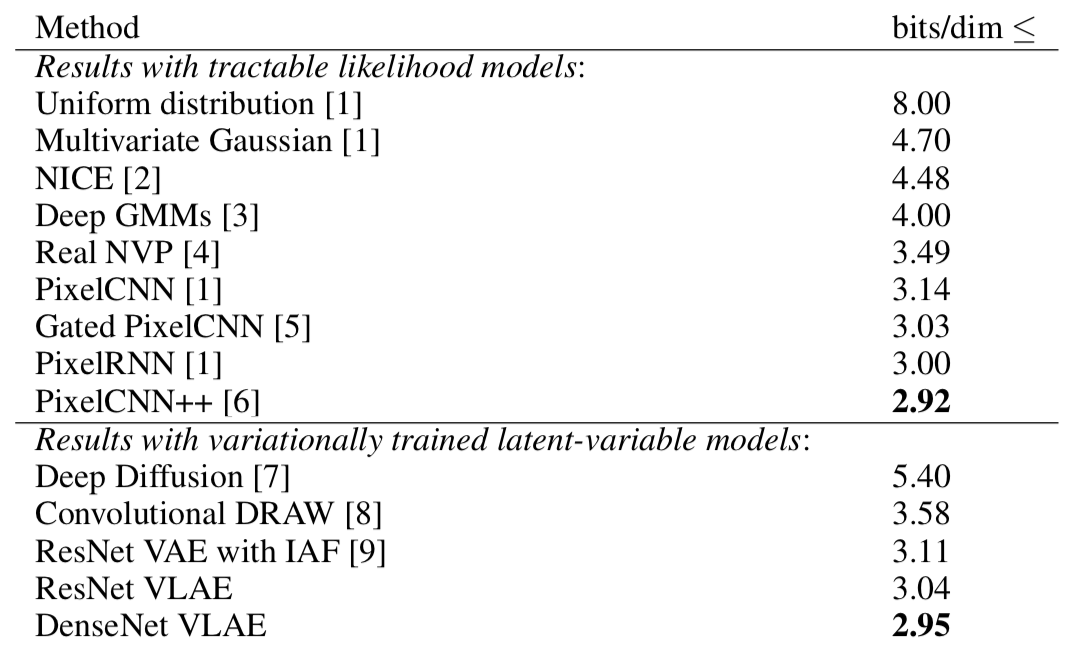
\includegraphics[width=1.\linewidth]{figs/VLAE_2.png}
		\end{figure}
	\end{minipage}
	
	\myfootnotewithlink{https://arxiv.org/abs/1611.02731}{Chen X. et al. Variational Lossy Autoencoder, 2016}
\end{frame}
%=======
\section{Flows intuition}
%=======
\begin{frame}{Flows intuition}
	Let $\xi$ be a random variable with density $p(\xi)$. Then
	\[
	\eta = F(\xi) = \int_{-\infty}^\xi p(t)dt \sim U[0, 1].
	\]
	\[
	P(\eta < y) = P(F(\xi) < y) = P(\xi < F^{-1}(y)) = F(F^{-1}(y)) = y
	\]
	Hence
	\[
	\eta \sim U[0, 1]; \quad \xi = F^{-1}(\eta) \quad \Rightarrow \quad \xi \sim p(\xi).
	\]
	\begin{figure}
		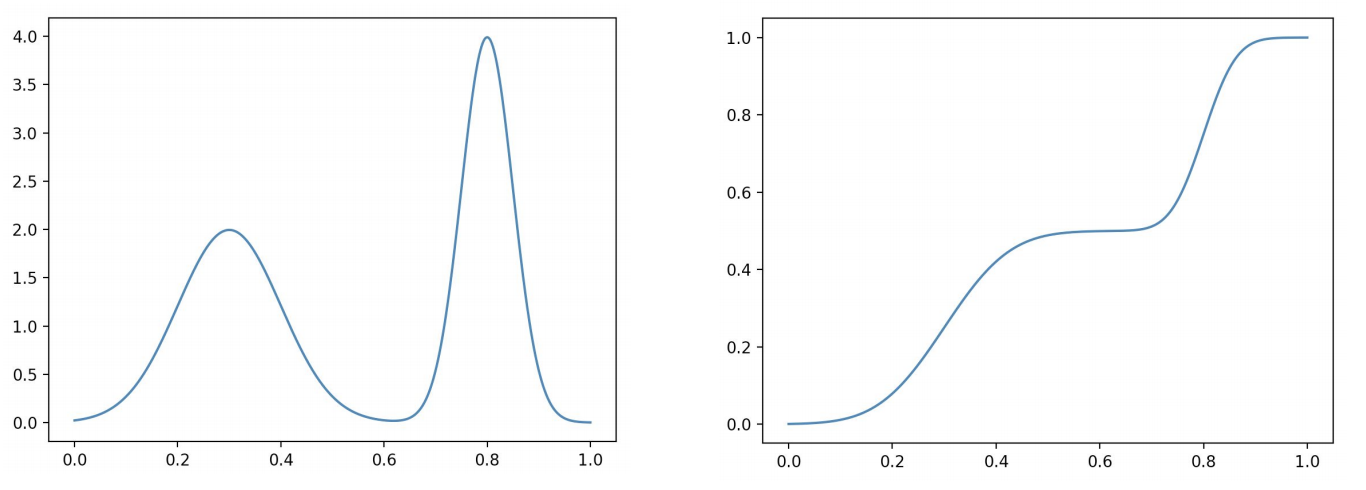
\includegraphics[width=\linewidth]{figs/flows_1d}
	\end{figure}
	\myfootnotewithlink{https://sites.google.com/view/berkeley-cs294-158-sp19/home}{image credit: https://sites.google.com/view/berkeley-cs294-158-sp19/home}
	
\end{frame}
%=======
\begin{frame}{Flows intuition}
	\begin{itemize}
		\item Let $z \sim p(z)$ is a random variable with base distribution $p(z) = U[0, 1]$. 
		\item Let $x \sim p(x)$ is a random variable with complex distribution $p(x)$ and cdf $F(x)$. 
		\item Then noise variable $z$ can be transformed to $x$ using inverse cdf~$F^{-1}$ ($x = F^{-1}(z)$).
	\end{itemize}
	How to transform random variable $z$  which has a distribution different from uniform to $x$?
	\begin{itemize}
		\item Let $z \sim p(z)$ is a random variable with base distribution $p(z)$ and cdf $G(z)$.
		\item Then $z_0 = G(z)$ has base distribution $p(z_0) = U[0, 1]$.
		\item Let $x \sim p(x)$ is a random variable with complex distribution $p(x)$ and cdf $F(x)$. 
		\item Then noise variable $z$ can be transformed to $x$ using cdf $G$ and inverse cdf~$F^{-1}$ ($x = F^{-1}(z_0) = F^{-1}(G(z))$).
	\end{itemize}
\end{frame}
%=======
\section{Parallel WaveNet}
%=======
\begin{frame}{MAF/IAF pros and cons}
	\begin{minipage}{0.50\columnwidth}
		\begin{block}{MAF}
			\begin{itemize}
				\item Sampling is slow.
				\item Likelihood evaluation is fast.
			\end{itemize}
		\end{block}
	\end{minipage}%
	\begin{minipage}{0.51\columnwidth}
		\begin{block}{IAF}
			\begin{itemize}
				\item Sampling is fast.
				\item Likelihood evaluation is slow.
			\end{itemize}
		\end{block}
	\end{minipage}
	How to take the best of both worlds?
	\begin{block}{WaveNet}
		Autoregressive model with caused dilated convolutions for raw audio waveforms generation.
		\vspace{-0.5cm}
		\[
			p(\bx| \btheta) = \prod_{t=1}^T p(x_t|\bx_{1:t-1}, \btheta).
		\]
		\vspace{-0.7cm}
		\begin{figure}
			\centering
			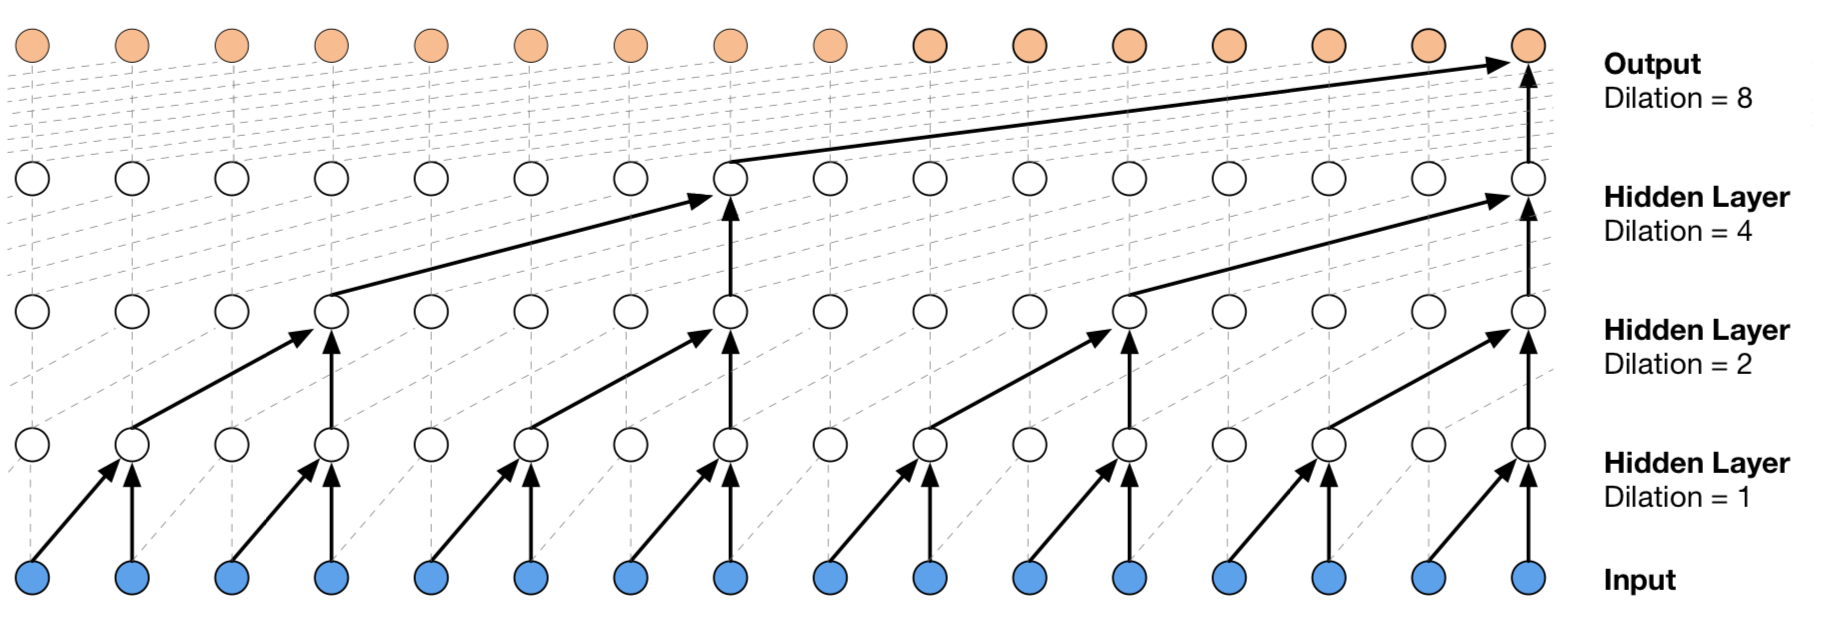
\includegraphics[width=0.85\linewidth]{figs/wavenet2.png}
		\end{figure}
	\end{block}
	\myfootnotewithlink{https://arxiv.org/abs/1609.03499}{Oord A. et al. Wavenet: A generative model for raw audio, 2016}
\end{frame}
%=======
\begin{frame}{Parallel WaveNet}
	\begin{itemize}
		\item 24kHz instead of 16kHz using increased dilated convolution filter size from 2 to 3.
		\item 16-bit signals with mixture of logistics instead of 8-bit signal with 256-way categorical distribution.
	\end{itemize}
	\begin{block}{Probability density distillation}
		\begin{enumerate}
			\item Train usual WaveNet (MAF) via MLE (teacher network).
			\item Train IAF WaveNet (student network), which attempts to match the probability of its own samples under the distribution learned by the teacher.
		\end{enumerate}
	\end{block}
	\vspace{-0.3cm}
	\begin{block}{Student objective}
		\vspace{-0.3cm}
		\[
			KL(p_s || p_t) = H(p_s, p_t) - H(p_s).
		\]
		\vspace{-0.3cm}
	\end{block}
	More than 1000x speed-up relative to original WaveNet!
	\myfootnotewithlink{https://arxiv.org/abs/1711.10433}{Oord A. et al. Parallel WaveNet: Fast High-Fidelity Speech Synthesis, 2017}
\end{frame}
%=======
\begin{frame}{Parallel WaveNet}
	\begin{figure}
		\centering
		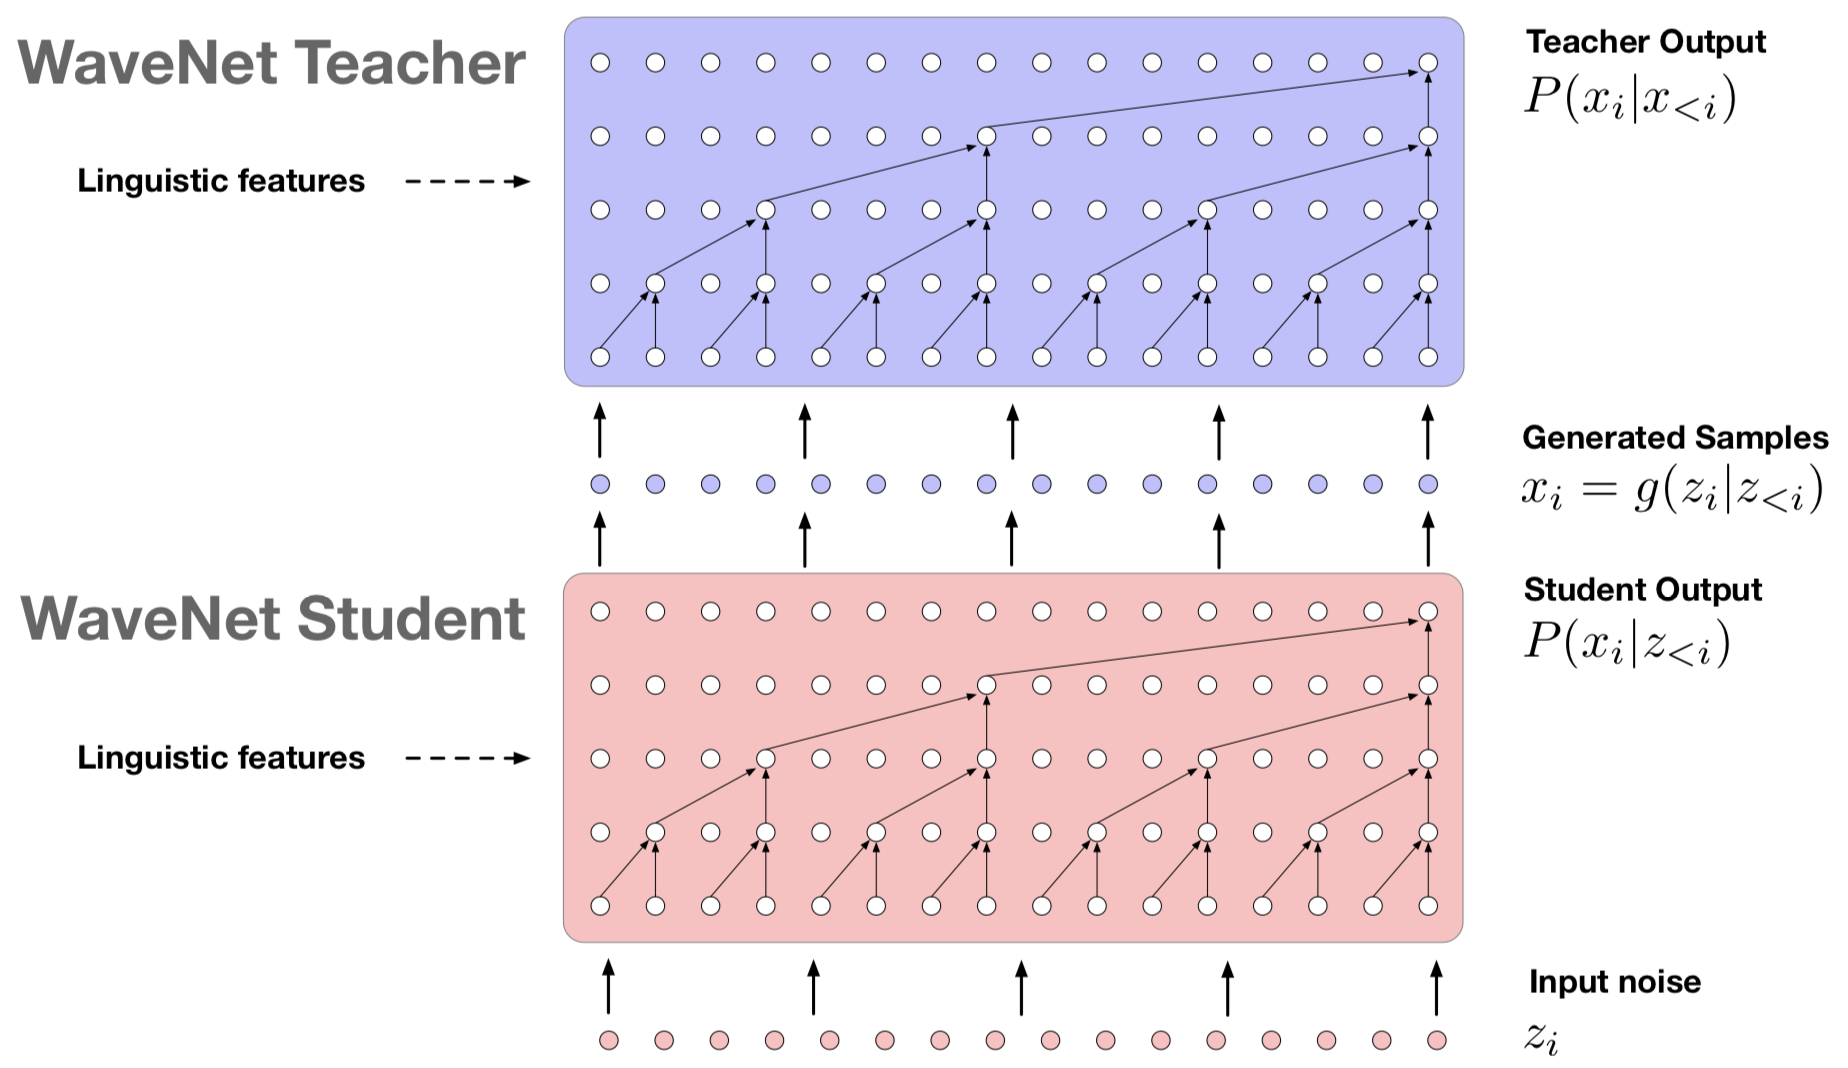
\includegraphics[width=\linewidth]{figs/parallel_wavenet.png}
	\end{figure}

	\myfootnotewithlink{https://arxiv.org/abs/1711.10433}{Oord A. et al. Parallel WaveNet: Fast High-Fidelity Speech Synthesis, 2017}
\end{frame}
%=======
\section{RevNet, i-RevNet}
%=======
\begin{frame}{RevNets, 2017}
	\begin{minipage}[t]{0.6\columnwidth}
		\begin{itemize}
			\item Modern neural networks are trained via backpropagation.
			\item Residual networks are state of the art in image classification.
			\item Backpropagation requires storing the network activations.
		\end{itemize}
	\end{minipage}%
	\begin{minipage}[t]{0.4\columnwidth}
		\begin{figure}
			\centering
			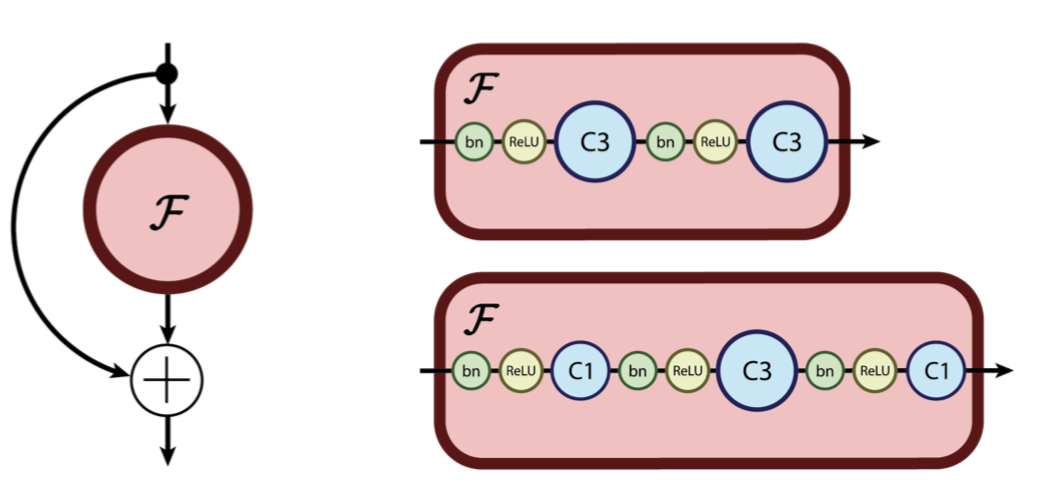
\includegraphics[width=\linewidth]{figs/resnet_block.png}
		\end{figure}
	\end{minipage}
	\vspace{0.1cm}
	\begin{block}{Problem}
		Storing the activations imposes an increasing memory burden. GPUs have limited memory capacity, leading to constraints often exceeded by state-of-the-art architectures (with thousand layers).
	\end{block}
	\myfootnotewithlink{https://arxiv.org/abs/1707.04585}{Gomez A. N. et al. The Reversible Residual Network: Backpropagation Without Storing Activations, 2017}
\end{frame}
%=======
\begin{frame}{RevNets, 2017}
	\begin{block}{NICE}
		\vspace{-0.2cm}
		\begin{equation*}
			\begin{cases} \bz_1 = \bx_1; \\ \bz_2 = \bx_2 + \mathcal{F}(\bx_1, \btheta);\end{cases}  \quad \Leftrightarrow \quad 
			\begin{cases} \bx_1 = \bz_1; \\ \bx_2 = \bz_2 - \mathcal{F}(\bz_1, \btheta).\end{cases} 
		\end{equation*}
		\vspace{-0.2cm}
	\end{block}
	\begin{block}{RevNet}
		\begin{equation*}
			\begin{cases} \by_1 = \bx_1 + \mathcal{F}(\bx_2, \btheta); \\ \by_2 = \bx_2 + \mathcal{G}(\by_1, \btheta);\end{cases} \quad \Leftrightarrow \quad 
			\begin{cases} \bx_2 = \by_2 - \mathcal{F}(\by_1, \btheta); \\ \bx_1 = \by_1 - \mathcal{G}(\bx_2, \btheta).\end{cases} 
		\end{equation*}
	\end{block}
	\begin{figure}
		\centering
		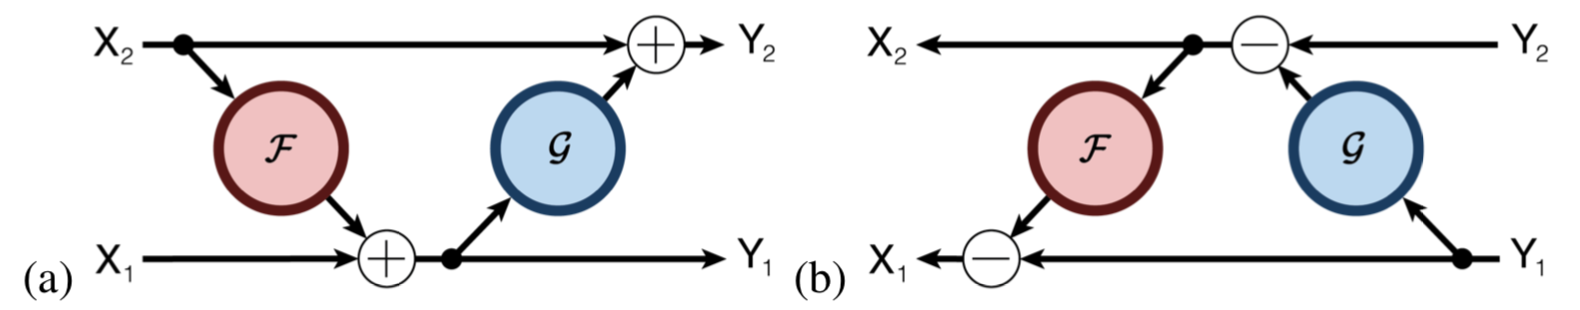
\includegraphics[width=\linewidth]{figs/revnet.png}
	\end{figure}
	\myfootnotewithlink{https://arxiv.org/abs/1707.04585}{Gomez A. N. et al. The Reversible Residual Network: Backpropagation Without Storing Activations, 2017}
\end{frame}
%=======
\begin{frame}{RevNets, 2017}
	\begin{figure}
		\centering
		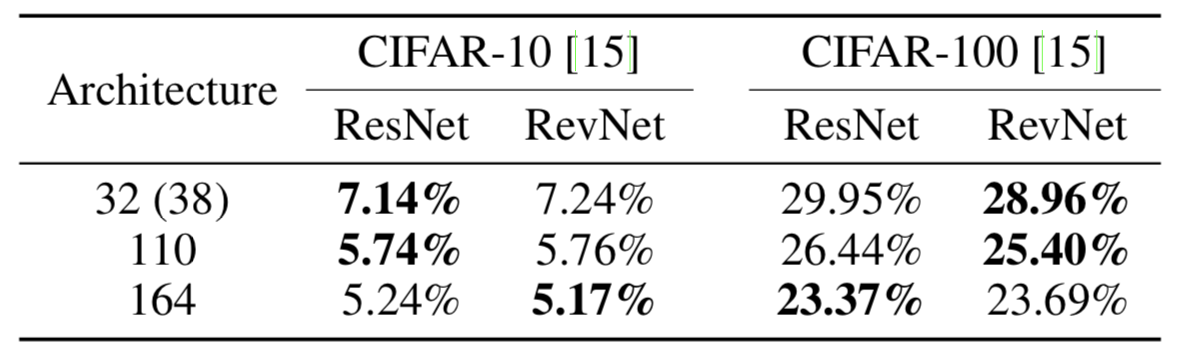
\includegraphics[width=0.8\linewidth]{figs/revnet_results.png}
	\end{figure}
	\begin{itemize}
		\item If the network contains non-reversible blocks (poolings, strides), activations for these blocks should be stored.
		\item To avoid storing activations in the modern frameworks, the backward pass should be manually redefined.
	\end{itemize}
	\myfootnotewithlink{https://arxiv.org/abs/1707.04585}{Gomez A. N. et al. The Reversible Residual Network: Backpropagation Without Storing Activations, 2017}
\end{frame}
%=======
\begin{frame}{i-RevNet, 2018}
	\begin{block}{Hypothesis}
		The success of deep convolutional networks is based on progressively discarding uninformative variability about the input with respect to the problem at hand. 
	\end{block}
	\begin{itemize}
		\item It is difficult to recover images from their hidden representations. 
		\item Information bottleneck principle: an optimal representation must reduce the MI between an input and its representation to reduce uninformative variability + maximize the MI between the output and its representation to preserve each class from collapsing onto other classes.
	\end{itemize}
	\myfootnotewithlink{https://arxiv.org/abs/1802.07088}{Jacobsen J. H., Smeulders A., Oyallon E. i-RevNet: Deep Invertible Networks, 2018}
\end{frame}
%=======
\begin{frame}{i-RevNet, 2018}
	\begin{block}{Hypothesis}
		The success of deep convolutional networks is based on progressively discarding uninformative variability about the input with respect to the problem at hand. 
	\end{block}
	
	\begin{block}{Idea}
		Build a cascade of homeomorphic layers (i-RevNet), a network that can be fully inverted up to the final projection onto the classes, i.e. no information is discarded.
	\end{block}
	\myfootnotewithlink{https://arxiv.org/abs/1802.07088}{Jacobsen J. H., Smeulders A., Oyallon E. i-RevNet: Deep Invertible Networks, 2018}
\end{frame}
%=======
\begin{frame}{i-RevNet, 2018}
	
	\begin{figure}
		\centering
		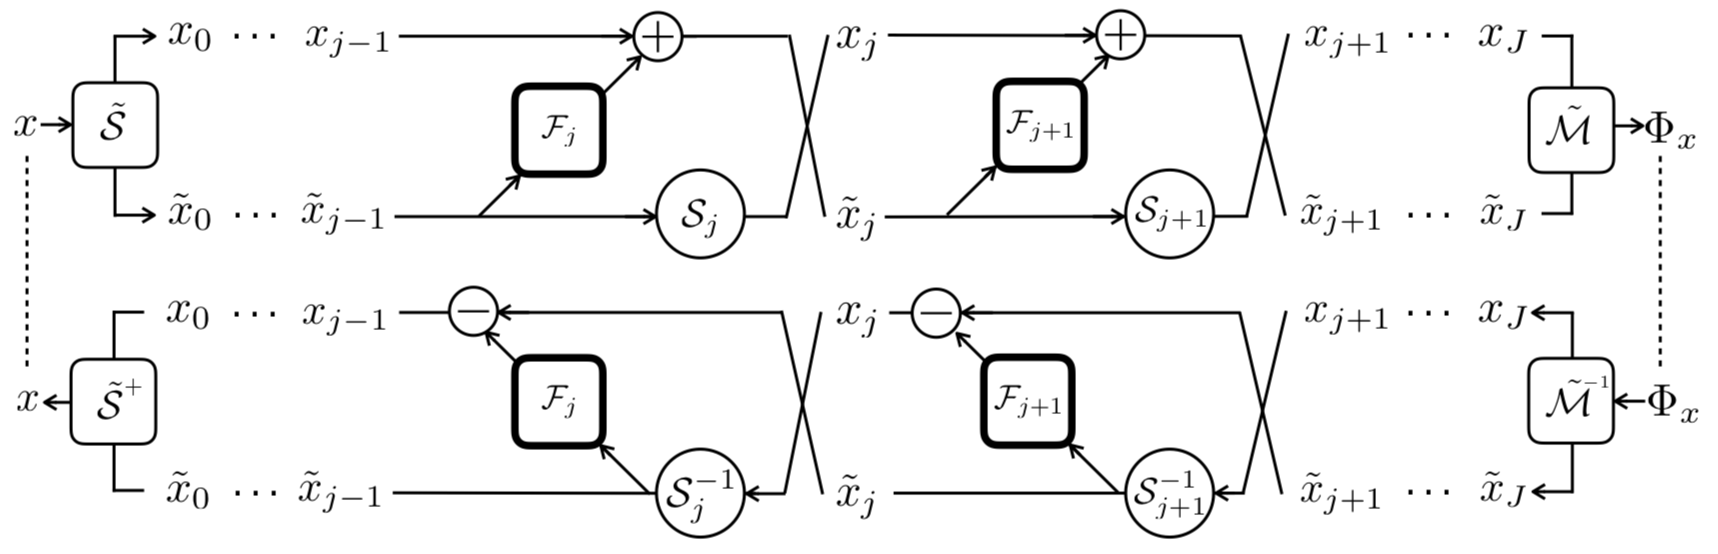
\includegraphics[width=\linewidth]{figs/i-revnet.png}
	\end{figure}
	
	\begin{figure}
		\centering
		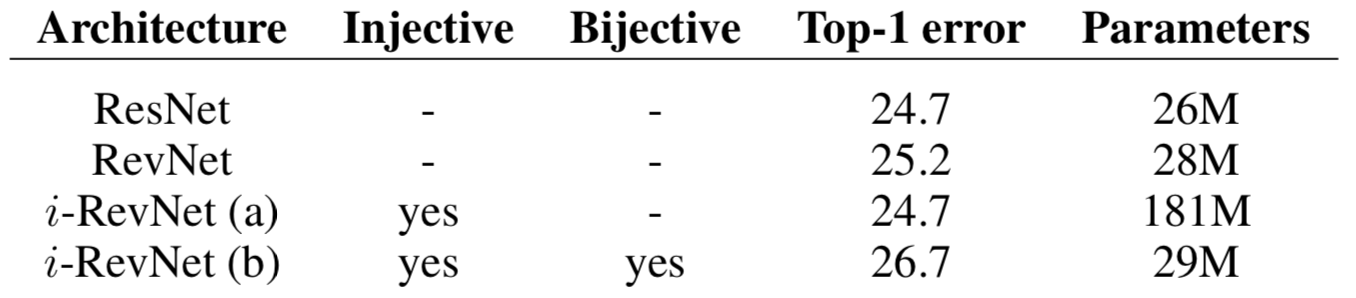
\includegraphics[width=0.9\linewidth]{figs/i-revnet_block.png}
	\end{figure}

	\myfootnotewithlink{https://arxiv.org/abs/1802.07088}{Jacobsen J. H., Smeulders A., Oyallon E. i-RevNet: Deep Invertible Networks, 2018}
\end{frame}
%=======
\section{ELBO surgery}
%=======
\begin{frame}{ELBO interpretations}
	\[
		\log p(\bx | \btheta) = \cL (q, \btheta) + KL(q(\bz | \bx, \bphi) || p(\bz | \bx, \btheta)).
	\]
	\[
		\cL (q, \btheta) = \int q(\bz | \bx, \bphi) \log \frac{p(\bx, \bz | \btheta)}{q(\bz | \bx, \bphi)} d \bz.
	\]
	\begin{itemize}
	    \item Evidence minus posterior KL
	    \vspace{-0.1cm}
	    \[
	        \mathcal{L}(q, \btheta) = \log p(\bx | \btheta) - KL(q(\bz | \bx, \bphi) || p(\bz | \bx, \btheta)).
	    \]
	    \item Average negative energy plus entropy
	    \vspace{-0.1cm}
	    \begin{align*}
	        \mathcal{L}(q, \btheta) &= \mathbb{E}_{q(\bz | \bx, \bphi)} \left[\log p(\bx, \bz | \btheta) - \log q(\bz | \bx, \bphi)  \right] \\
	        &= \mathbb{E}_{q(\bz | \bx, \bphi)} \log p(\bx, \bz | \btheta) + \mathbb{H} \left[q(\bz | \bx, \bphi) \right].
	    \end{align*}
	    \item Average reconstruction minus KL to prior
	    \vspace{-0.1cm}
	    \begin{align*}
	        \mathcal{L}(q, \btheta) &= \mathbb{E}_{q(\bz | \bx, \bphi)} \left[ \log p(\bx | \bz, \btheta) + \log p(\bz) - \log q(\bz | \bx, \bphi) \right] \\
	        &= \mathbb{E}_{q(\bz | \bx, \bphi)} \log p(\bx | \bz, \btheta) - KL(q(\bz | \bx, \bphi) || p(\bz)).
	    \end{align*}
	\end{itemize}
\end{frame}
%=======
\begin{frame}{ELBO surgery, 2016}
		\[
			\mathcal{L} (q, \btheta)  = \int q(\bZ | \bX) \log \frac{p(\bX, \bZ | \btheta)}{q(\bZ | \bX)} d\bZ.
		\]
		\vspace{-0.1cm}
	\begin{block}{ELBO interpretations}
	\begin{itemize}
	    \item Evidence minus posterior KL
	    \vspace{-0.1cm}
	    \[
	        \mathcal{L}(q, \btheta) = \log p(\bX | \btheta) - KL(q(\bZ | \bX) || p(\bZ | \bX, \btheta)).
	    \]
	    \item Average negative energy plus entropy
	    \vspace{-0.1cm}
	    \[
	        \mathcal{L}(q, \btheta) = \mathbb{E}_{q(\bZ | \bX)} p(\bX, \bZ | \btheta) + \mathbb{H} \left[q(\bZ | \bX) \right].
	    \]
	    \item Average term-by-term reconstruction minus KL to prior
	    \vspace{-0.1cm}
	    \[
	        \mathcal{L}(q, \btheta) = \frac{1}{n} \sum_{i=1}^n \left[ \mathbb{E}_{q(\bz_i | \bx_i)} \log p(\bx_i | \bz_i, \btheta) - KL(q(\bz_i | \bx_i) || p(\bz_i)) \right].
	    \]
	\end{itemize}
	\end{block}
	
	\vfill
	\hrule\medskip
	{\scriptsize \href{http://approximateinference.org/accepted/HoffmanJohnson2016.pdf}{http://approximateinference.org/accepted/HoffmanJohnson2016.pdf}}
\end{frame}
%=======
\begin{frame}{ELBO surgery, 2016}
\vspace{-0.3cm}
\[
    \mathcal{L}(q, \btheta) = \frac{1}{n} \sum_{i=1}^n \left[ \mathbb{E}_{q(\bz_i | \bx_i)} \log p(\bx_i | \bz_i, \btheta) - KL(q(\bz_i | \bx_i) || p(\bz_i)) \right].
\]
\vspace{-0.3cm}
\begin{block}{Theorem}
\[
    \frac{1}{n} \sum_{i=1}^n KL(q(\bz_i | \bx_i) || p(\bz_i)) = KL(q(\bz) || p(\bz)) + \mathbb{I}_{q(i, \bz)} [i, \bz],
\]
where $i$ is treated as random variable:
\footnotesize{
\[
    q(i, \bz) = q(i) q(\bz | i); \quad p(i, \bz) = p(i) p(\bz); \quad 
    q(i) = p(i) = \frac{1}{n}; \quad q(\bz | i) = q(\bz | \bx_i).
\]
\[
    q(\bz) = \sum_{i=1}^n q(i, \bz) = \frac{1}{n} \sum_{i=1}^n q(\bz | \bx_i); \quad  \mathbb{I}_{q(i, \bz)} [i, \bz] = \mathbb{E}_{q(i, \bz)} \log \frac{q(i, \bz)}{q(i)q(\bz)}.
\]
}
\end{block}

\vfill
\hrule\medskip
{\scriptsize \href{http://approximateinference.org/accepted/HoffmanJohnson2016.pdf}{http://approximateinference.org/accepted/HoffmanJohnson2016.pdf}}
\end{frame}
%=======
\begin{frame}{ELBO surgery, 2016}
\begin{block}{Theorem}
\[
    \frac{1}{n} \sum_{i=1}^n KL(q(\bz_i | \bx_i) || p(\bz_i)) = KL(q(\bz) || p(\bz)) + \mathbb{I}_{q(i, \bz)} [i, \bz].
\]
\end{block}
\begin{block}{Proof}
\vspace{-0.3cm}
{\footnotesize
\begin{multline*}
    \frac{1}{n} \sum_{i=1}^n KL(q(\bz_i | \bx_i) || p(\bz_i)) = \sum_{i=1}^n \int q(i) q(\bz | i) \log \frac{q(\bz | i)}{p(\bz)} d \bz = \\
    = \sum_{i=1}^n \int q(i, \bz) \log \frac{q(i, \bz)}{p(\bz)p(i)} d \bz =
    \int \sum_{i=1}^n q(i, \bz) \log \frac{ q (\bz) q(i | \bz) }{p(\bz) p(i) } d \bz = \\
    = \int q(\bz) \log \frac{q(\bz)}{p(\bz)} d\bz + \int \sum_{i=1}^n q(i | \bz) q(\bz) \log \frac{q(i | \bz)}{p(i)} d \bz = \\
    = KL (q(\bz) || p(\bz)) - \mathbb{E}_{q(\bz)} \mathbb{H} \left[q(i | \bz)  \right] + \log n.
\end{multline*}
}
\end{block}
\vfill
\hrule\medskip
{\scriptsize \href{http://approximateinference.org/accepted/HoffmanJohnson2016.pdf}{http://approximateinference.org/accepted/HoffmanJohnson2016.pdf}}
\end{frame}
%=======
\begin{frame}{ELBO surgery, 2016}
\begin{block}{Theorem}
\[
    \frac{1}{n} \sum_{i=1}^n KL(q(\bz_i | \bx_i) || p(\bz_i)) = KL(q(\bz) || p(\bz)) + \mathbb{I}_{q(i, \bz)} [i, \bz].
\]
\end{block}
\begin{block}{Proof (continued)}
{\footnotesize
\[
    \frac{1}{n} \sum_{i=1}^n KL(q(\bz_i | \bx_i) || p(\bz_i)) = KL (q(\bz) || p(\bz)) - \mathbb{E}_{q(\bz)} \mathbb{H} \left[q(i | \bz) \right] + \log n
\]
\begin{multline*}
    \mathbb{I}_{q(i, \bz)} [i, \bz] = \mathbb{E}_{q(i, \bz)} \log \frac{q(i, \bz)}{q(i)q(\bz)} = \mathbb{E}_{q(\bz)} \mathbb{E}_{q(i | \bz)} \log \frac{q(i | \bz) q(\bz)}{q(i)q(\bz)} = \\
    = \mathbb{E}_{q(\bz)} \mathbb{E}_{q(i | \bz)} \log \frac{q(i | \bz)}{q(i)} = - \mathbb{E}_{q(\bz)} \mathbb{H} \left[ q(i | \bz) \right] + \log n.
\end{multline*}
}
\end{block}
\vfill
\hrule\medskip
{\scriptsize \href{http://approximateinference.org/accepted/HoffmanJohnson2016.pdf}{http://approximateinference.org/accepted/HoffmanJohnson2016.pdf}}
\end{frame}
%=======
\begin{frame}{Learnable VAE prior}
	\begin{block}{Optimal prior}
		\vspace{-0.7cm}
		\[
			KL(q_{\text{agg}}(\bz) || p(\bz)) = 0 \quad \Leftrightarrow \quad p (\bz) = q_{\text{agg}}(\bz) = \frac{1}{n} \sum_{i=1}^n q(\bz | \bx_i).
		\]
		\vspace{-0.6cm}
	\end{block}
	\begin{block}{Mixture of Gaussians}
		\vspace{-0.3cm}
		\[
			p(\bz | \blambda) = \sum_{k=1}^K w_k \cN(\bz | \bmu_k, \bsigma_k^2), \quad \blambda = \{w_k, \bmu_k, \bsigma_k\}_{k=1}^K.
		\]
		\vspace{-0.5cm}
	\end{block}
	\begin{block}{Variational Mixture of posteriors (VampPrior)}
		\vspace{-0.3cm}
		\[
		p(\bz | \blambda) = \frac{1}{K} \sum_{k=1}^K q(\bz | \bu_k),
		\]
		where $\blambda = \{\bu_1, \dots, \bu_K\}$ are trainable pseudo-inputs.
	\end{block}
	\begin{itemize}
		\item Multimodal $\Rightarrow$ prevents over-regularization;.
		\item $K \ll n$ $\Rightarrow$ prevents from potential overfitting + less expensive to train.
	\end{itemize}
	\myfootnotewithlink{https://arxiv.org/abs/1705.07120}{Tomczak J. M., Welling M. VAE with a VampPrior, 2017}
\end{frame}
%=======
\begin{frame}{VampPrior}
	\begin{itemize}
	\item Do we really need the multimodal prior?
	\item Is it beneficial to couple the prior with the variational posterior or the MoG prior is enough?
	\end{itemize}
	\begin{block}{Results}
		\vspace{-0.3cm}
		\begin{minipage}[t]{0.55\columnwidth}
			\begin{figure}[h]
				\centering
				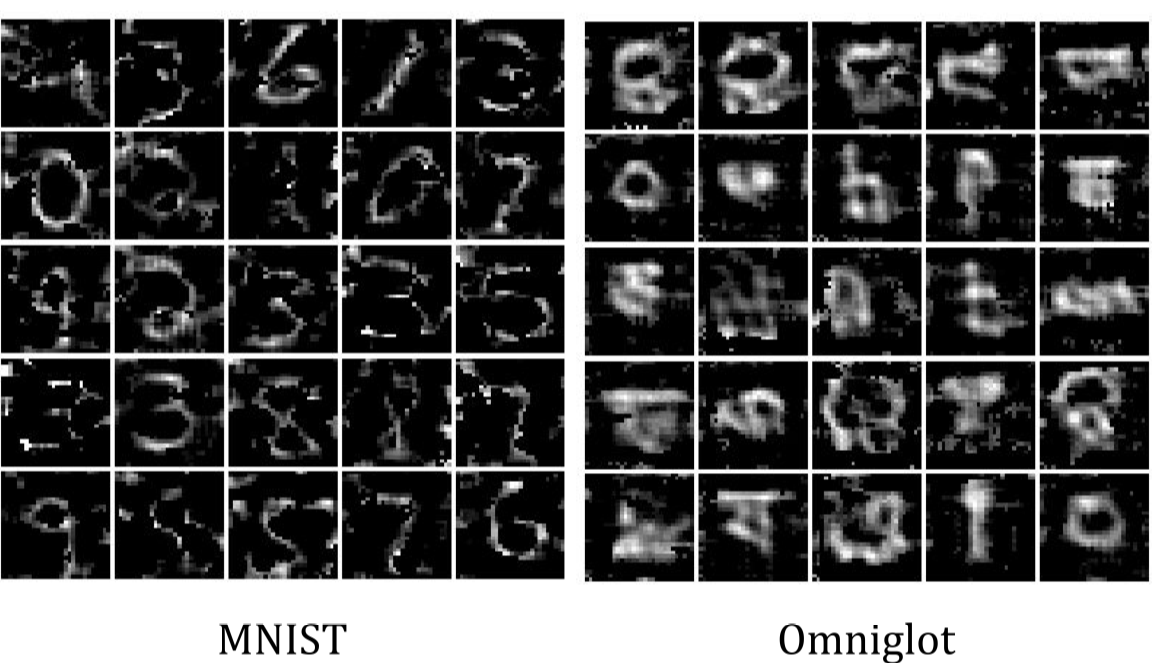
\includegraphics[width=1.0\linewidth]{figs/VampPrior_1.png}
			\end{figure}
		\end{minipage}%
		\begin{minipage}[t]{0.45\columnwidth}
			\begin{figure}[h]
				\centering
				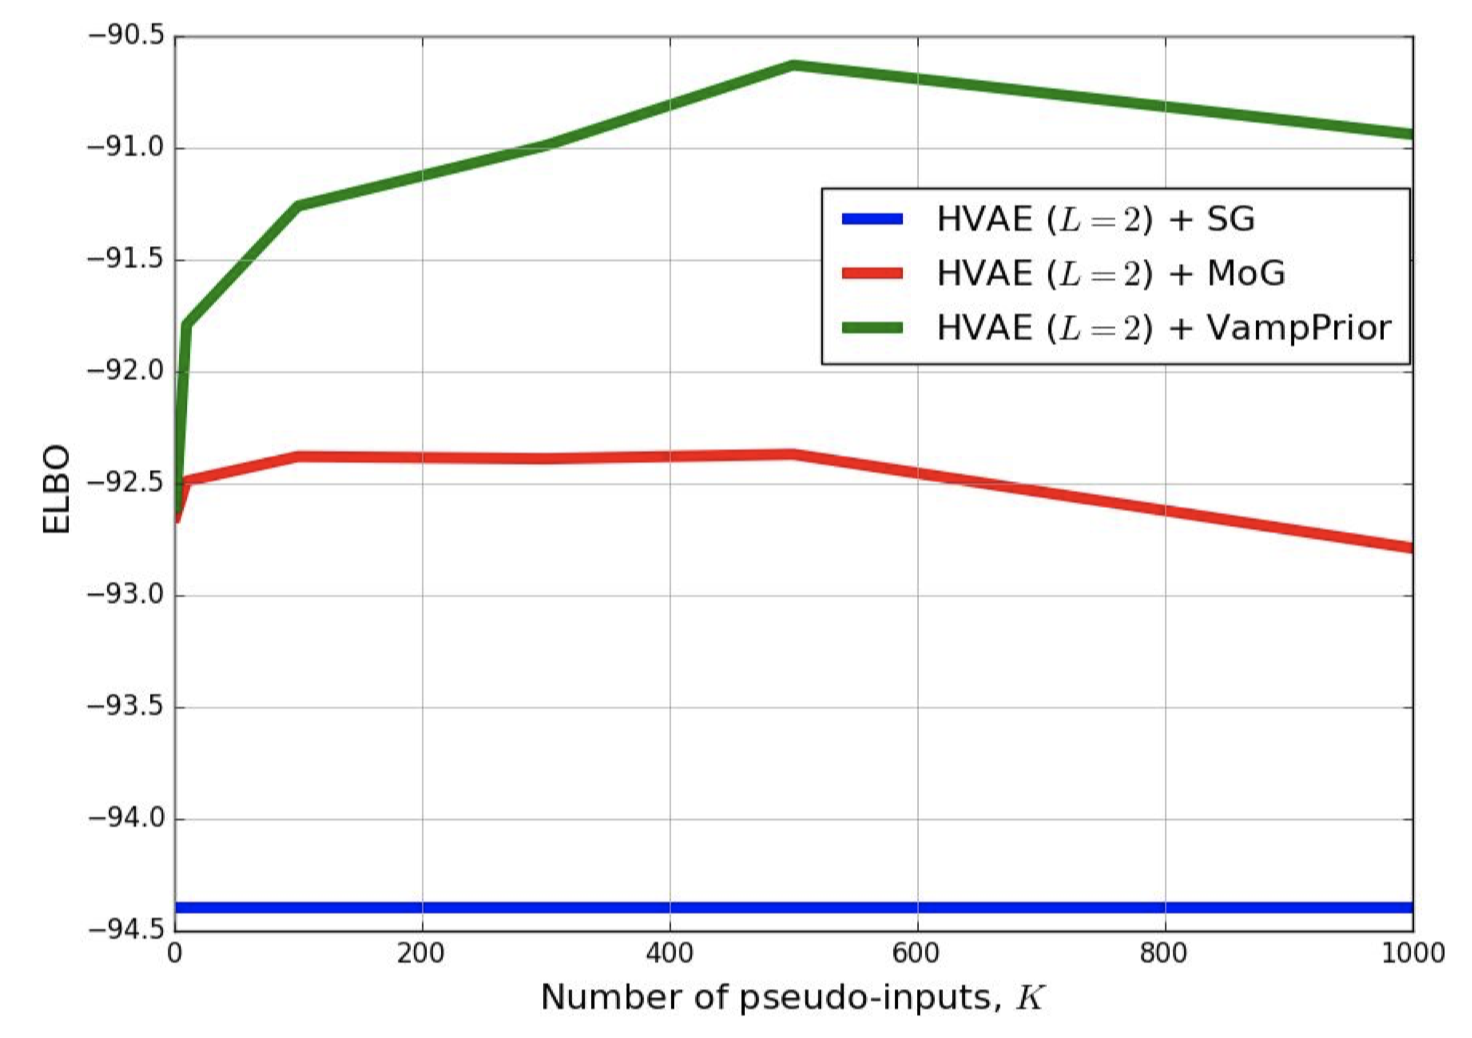
\includegraphics[width=1.0\linewidth]{figs/VampPrior_2.png}
			\end{figure}
		\end{minipage}
	\end{block}
	\textbf{Top row:} generated images by PixelHVAE + VampPrior for chosen pseudo-input in the left top corner. \\
	\vspace{0.1cm}
	\textbf{Bottom row:} pseudo-inputs for different datasets.
	\myfootnotewithlink{https://arxiv.org/abs/1705.07120}{Tomczak J. M., Welling M. VAE with a VampPrior, 2017}
\end{frame}
%=======
\section{Disentanglement}
%=======
\subsection{InfoGAN}
%=======
\begin{frame}{InfoGAN}
	\begin{block}{GAN objective}
		\vspace{-0.6cm}
		\[
		\min_{G} \max_D V(G, D)
		\]
		\[
		V(G, D)  =  \bbE_{\pi(\bx)} \log D(\bx) + \bbE_{p(\bz)} \log (1 - D(G(\bz)))
		\]
	\end{block}
	Latent vector $\bz$ is not imposed to be disentangled.
	
	InfoGAN decomposes input vector:
	\begin{itemize}
		\item $\bz$ -- incompressible noise;
		\item $\bc$ -- structured latent code $p(\bc) = \prod_{j=1}^d p(c_j)$.
	\end{itemize}
	\begin{block}{Information-theoretic regularization}
		\vspace{-0.3cm}
		\[
		\max I (\bc, G(\bz, \bc))
		\]
	\end{block}
	Information in the latent code $\bc$ should not be lost in the generation process.
	\myfootnotewithlink{https://arxiv.org/abs/1606.03657}{Chen X. et al. InfoGAN: Interpretable Representation Learning by Information Maximizing Generative Adversarial Nets, 2016}
\end{frame}
%=======
\begin{frame}{InfoGAN}
	\begin{block}{Objective}
		\vspace{-0.3cm}
		\[
		\min_{G} \max_D V(G, D) - \lambda I (\bc, G(\bz, \bc))
		\]
	\end{block}
	\begin{block}{Variational Information Maximization}
		\vspace{-0.3cm}
		\begin{multline*}
			I (\bc, G(\bz, \bc)) = H(\bc) - H(\bc | G(\bz, \bc)) = \\
			= H(\bc) + \bbE_{\bx \sim G(\bz, \bc)} \left[ \bbE_{\bc' \sim p(\bc | \bx)} \log p(\bc' | \bx) \right] = \\ 
			= H(\bc) + \bbE_{\bx \sim G(\bz, \bc)} KL(p(\bc'| \bx) || q(\bz' | \bx)) + 
			\\ + \bbE_{\bx \sim G(\bz, \bc)}  \bbE_{\bc' \sim p(\bc | \bx)} \log q(\bc' | \bx)  \geq\\
			\geq H(\bc) + \bbE_{\bx \sim G(\bz, \bc)} \bbE_{\bc' \sim p(\bc | \bx)} \log q(\bc' | \bx) = \\
			H(\bc) + \bbE_{\bc \sim p(\bc)} \bbE_{\bx \sim G(\bz, \bc)} \log q(\bc | \bx)
		\end{multline*}
	\end{block}
	\myfootnotewithlink{https://arxiv.org/abs/1606.03657}{Chen X. et al. InfoGAN: Interpretable Representation Learning by Information Maximizing Generative Adversarial Nets, 2016}
\end{frame}
%=======
\begin{frame}{InfoGAN}
	\begin{block}{Latent codes on MNIST}
		\begin{figure}
			\centering
			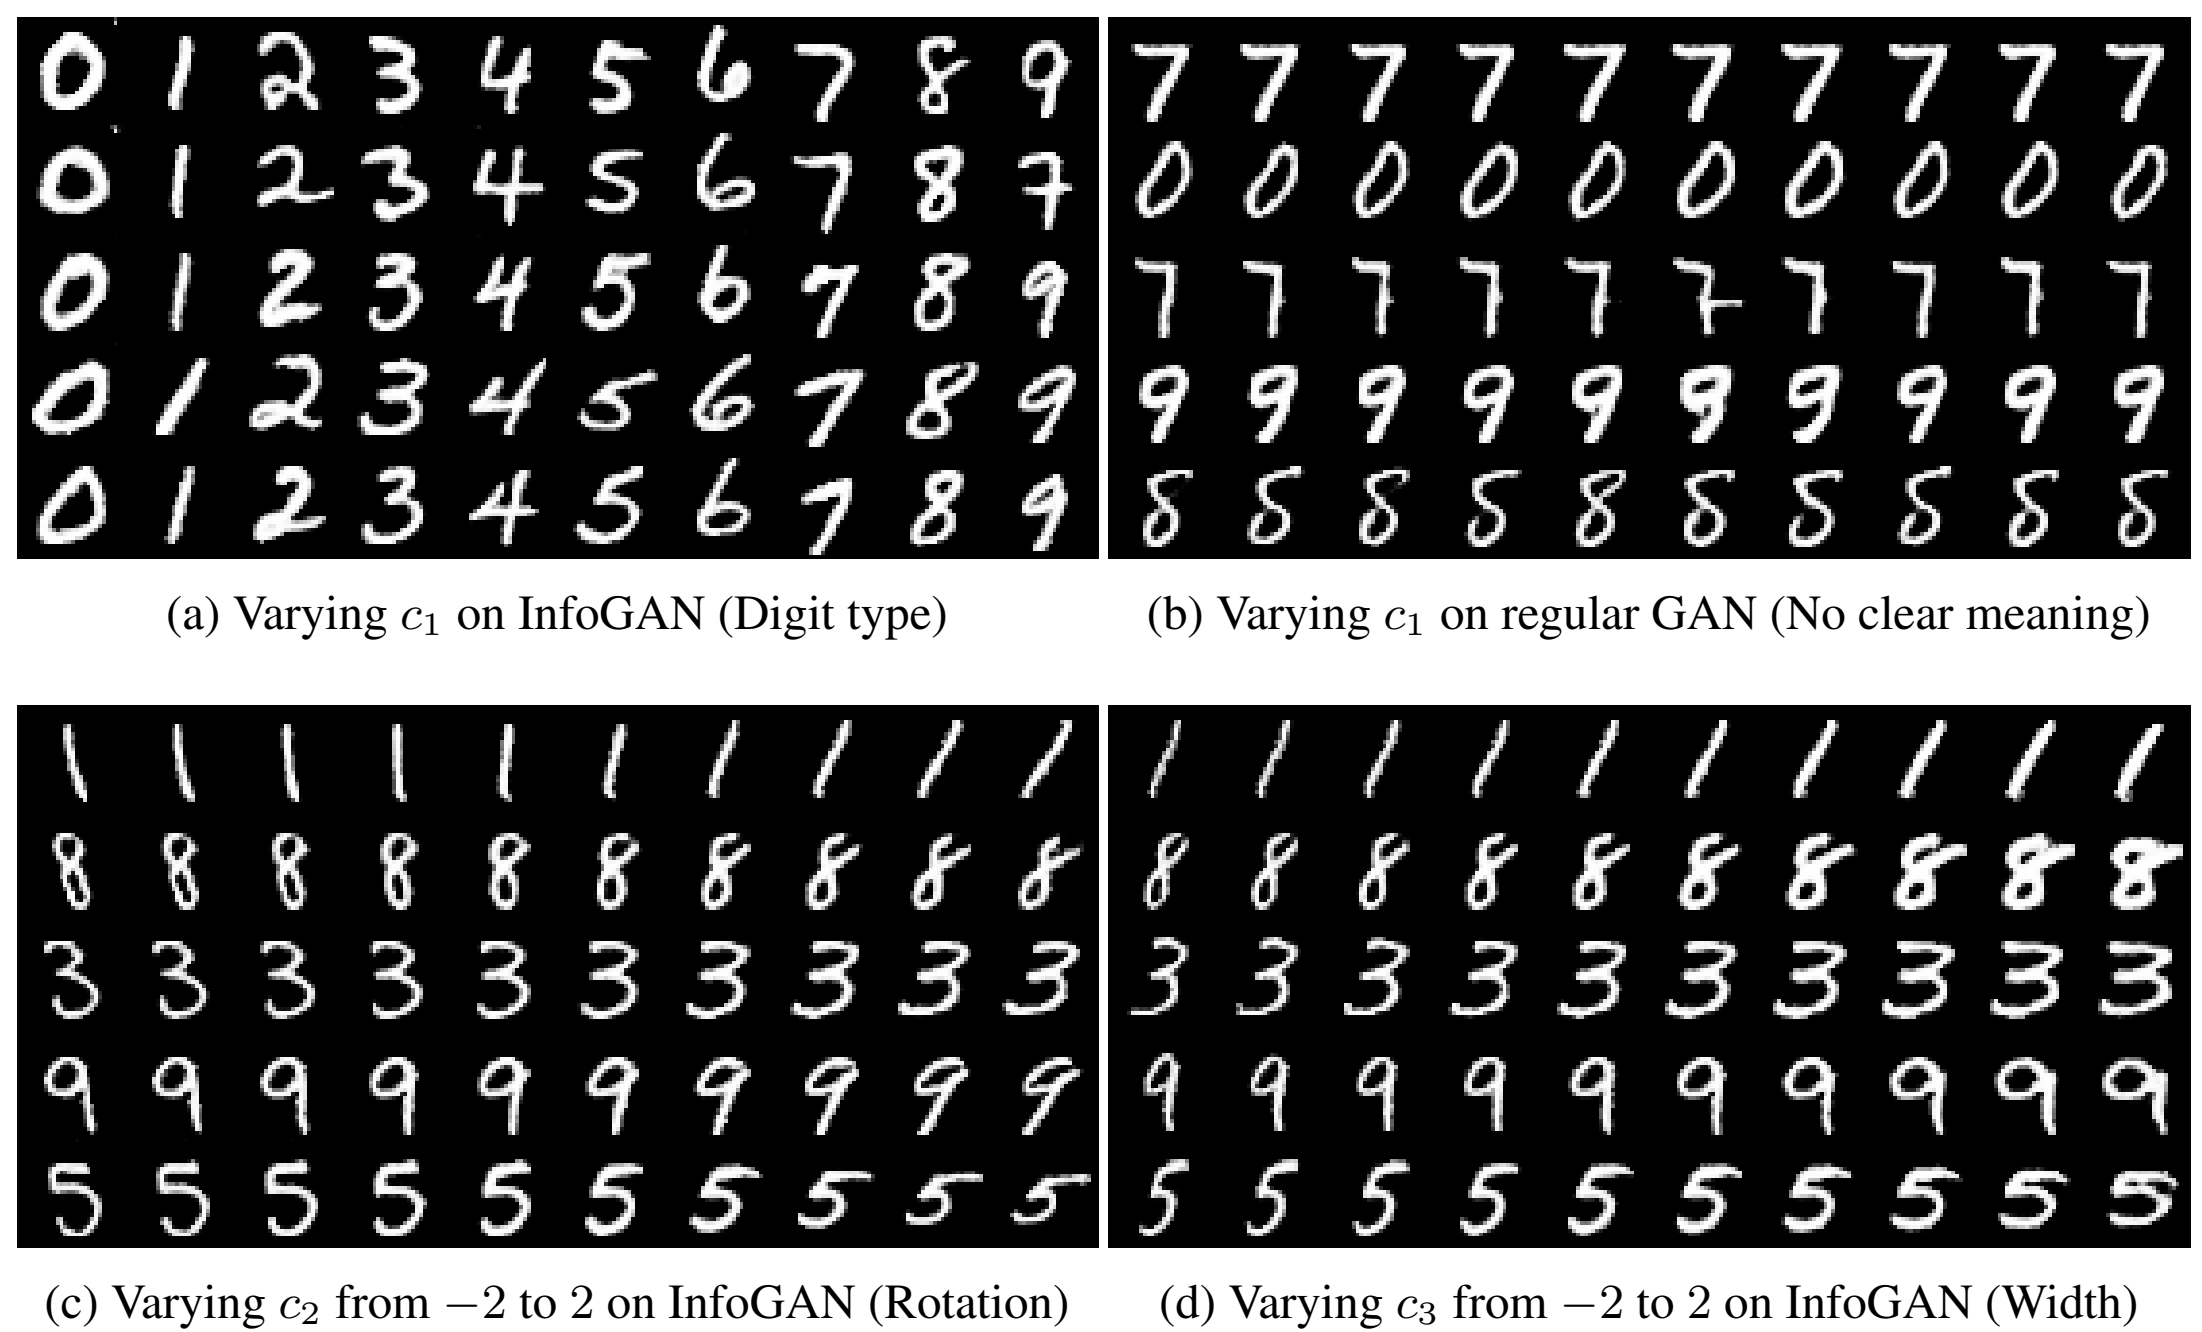
\includegraphics[width=\linewidth]{figs/infogan_mnist.png}
		\end{figure}
	\end{block}
	
	\myfootnotewithlink{https://arxiv.org/abs/1606.03657}{Chen X. et al. InfoGAN: Interpretable Representation Learning by Information Maximizing Generative Adversarial Nets, 2016}
\end{frame}
%=======
\begin{frame}{InfoGAN}
	\begin{block}{Latent codes on 3D Faces}
		\begin{figure}
			\centering
			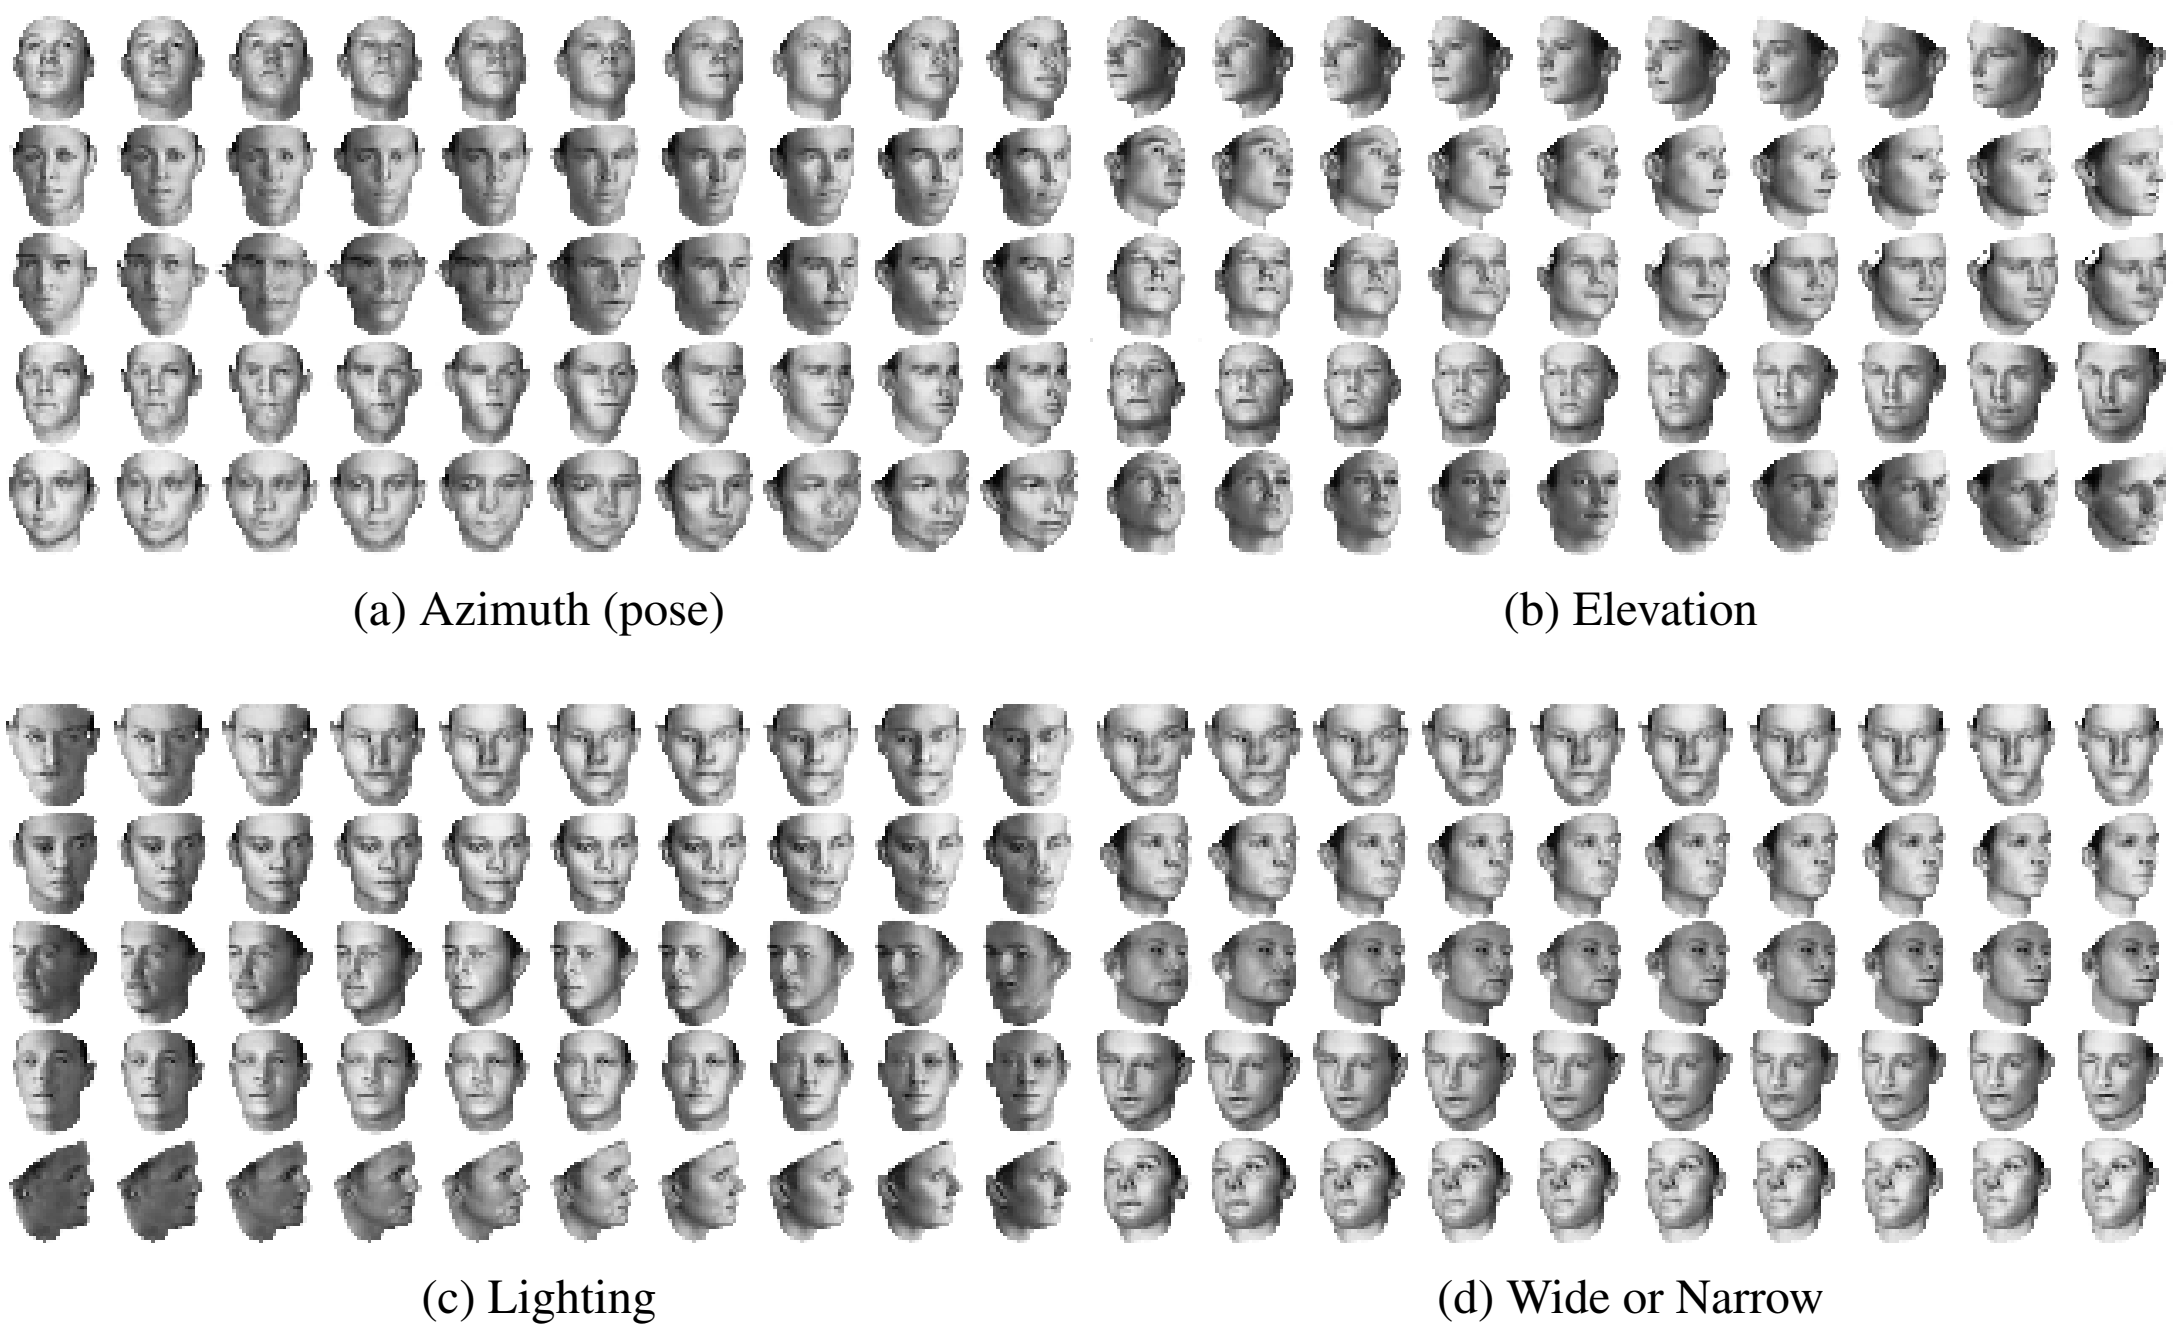
\includegraphics[width=\linewidth]{figs/infogan_faces.png}
		\end{figure}
	\end{block}
	
	\myfootnotewithlink{https://arxiv.org/abs/1606.03657}{Chen X. et al. InfoGAN: Interpretable Representation Learning by Information Maximizing Generative Adversarial Nets, 2016}
\end{frame}
%=======
\subsection{$\beta$-VAE, Disentanglement metric}
%=======
\begin{frame}{$\beta$-VAE}
	\begin{block}{Disentangling metric}
		\begin{enumerate}
			\item Generate two sets of objects
			\[
			\bx_{li} \sim \text{Sim}(\bv_{li}, \bw_{li}); \quad \bx_{lj} \sim \text{Sim}(\bv_{lj}, \bw_{lj}); \quad y_{ij} \sim U[1, d].
			\]
			\[
			\bv_{li} \sim p(\bv); \quad \bv_{lj} \sim p(\bv) \, ([v_{li}]_y = [v_{lj}]_y); \quad \bw_{li}, \bw_{lj} \sim p(\bw).
			\]
			\item Find representations
			\[
			q(\bz | \bx) = \mathcal{N}\left(\mu(\bx) | \sigma^2(\bx)\right); \quad \bz_{li} = \mu(\bx_{li}); \quad \bz_{lj} = \mu(\bx_{lj}).
			\]
			\item Use accuracy of classifier $p(y | \bz_{\text{diff}})$ with a low VC-dimension as metric of disentanglement
			\[
			\bz_{\text{diff}} = \frac{1}{L} \sum_{l=1}^L | \bz_{li} - \bz_{lj} |.
			\]
		\end{enumerate}
	\end{block}

	\myfootnotewithlink{https://openreview.net/references/pdf?id=Sy2fzU9gl}{Higgins I. et al. beta-VAE: Learning Basic Visual Concepts with a Constrained Variational Framework, 2017}
\end{frame}
%=======
\begin{frame}{$\beta$-VAE}
	\begin{itemize}
		\item \textbf{Top row:} original images.
		\item \textbf{Second row:} the corresponding reconstructions. 
		\item \textbf{Remaining rows:} latent traversals ordered by KL divergence with the prior. 
		\item \textbf{Heatmaps:} latent activations for each 2D position.
	\end{itemize}
	\begin{figure}
		\centering
		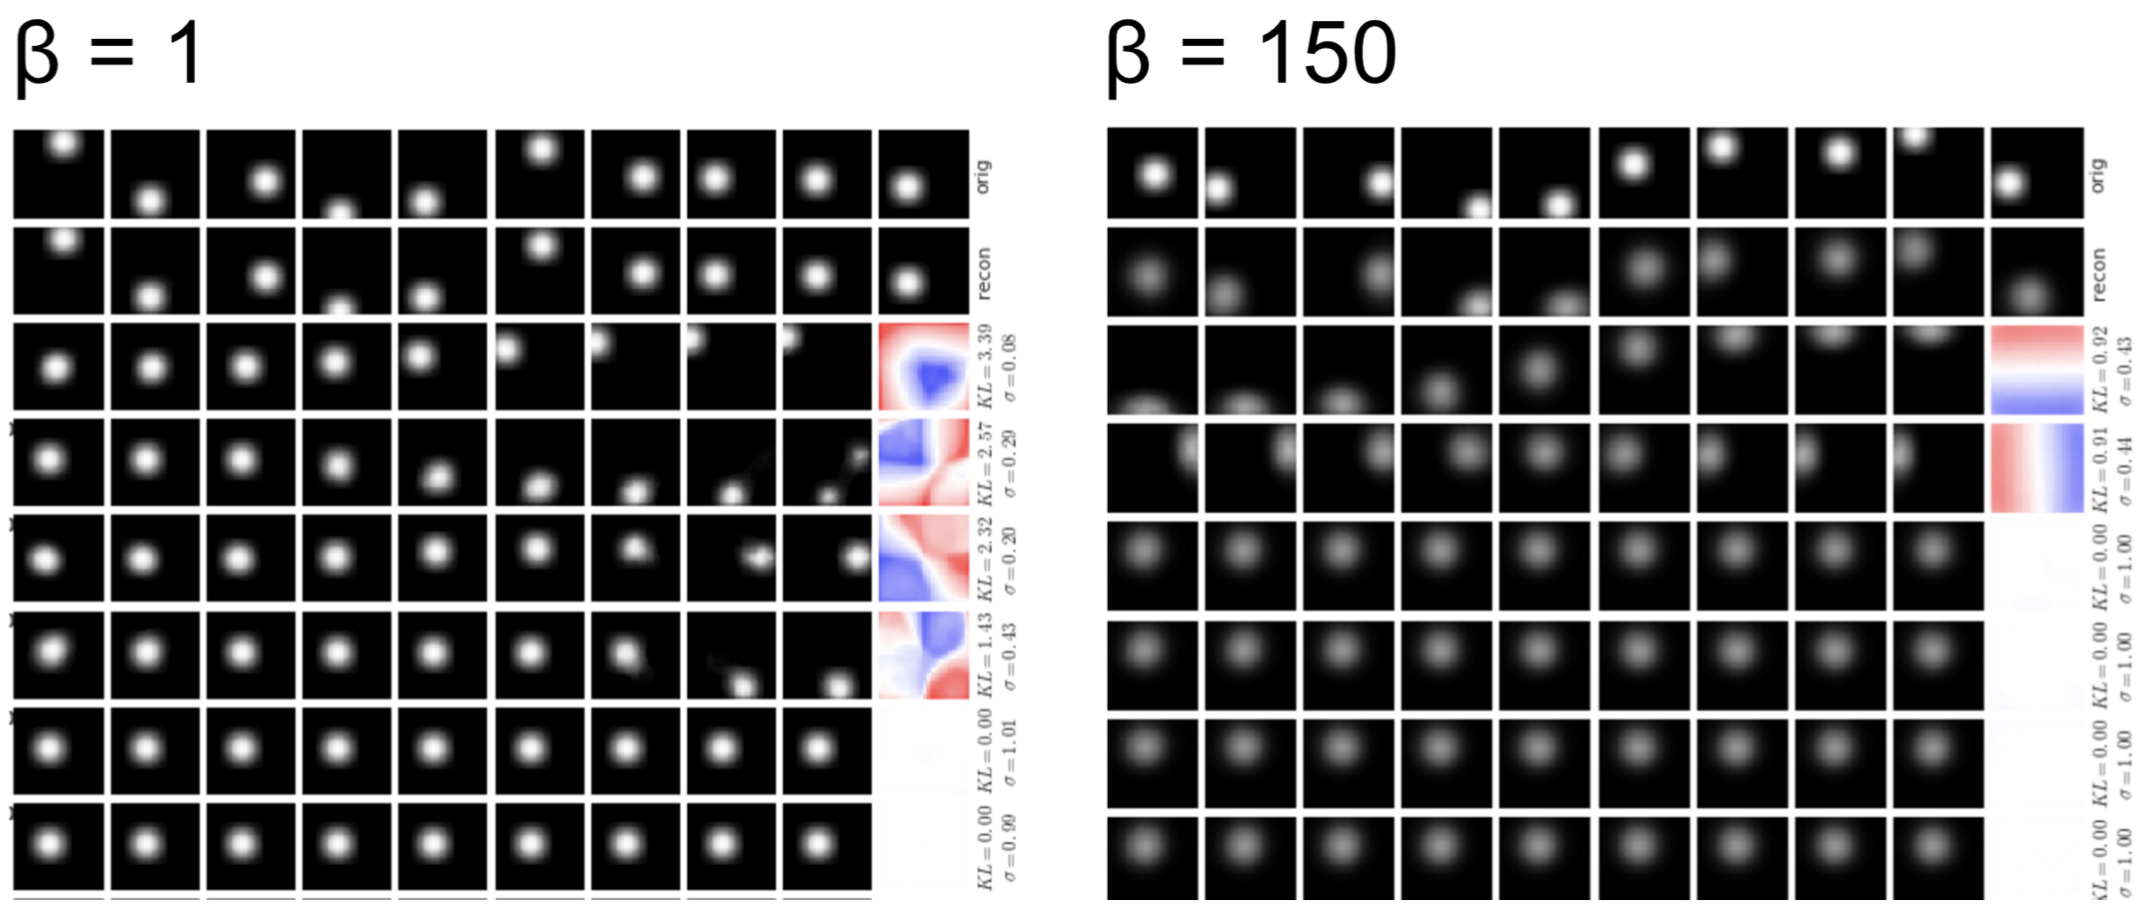
\includegraphics[width=\linewidth]{figs/betaVAE_6.png}
	\end{figure}

	\myfootnotewithlink{https://arxiv.org/abs/1804.03599}{Burgess C. P. et al. Understanding disentangling in $\beta$-VAE, 2018}
\end{frame}
%=======
\begin{frame}{$\beta$-VAE}
	\begin{block}{Controlled encoding capacity}
		\vspace{-0.5cm}
		\[
		\mathcal{L}(q, \btheta, \beta) = \mathbb{E}_{q(\bz | \bx)} \log p(\bx | \bz, \btheta) - | KL (q(\bz | \bx) || p(\bz)) - C|.
		\]
	\end{block}
	\begin{figure}
		\centering
		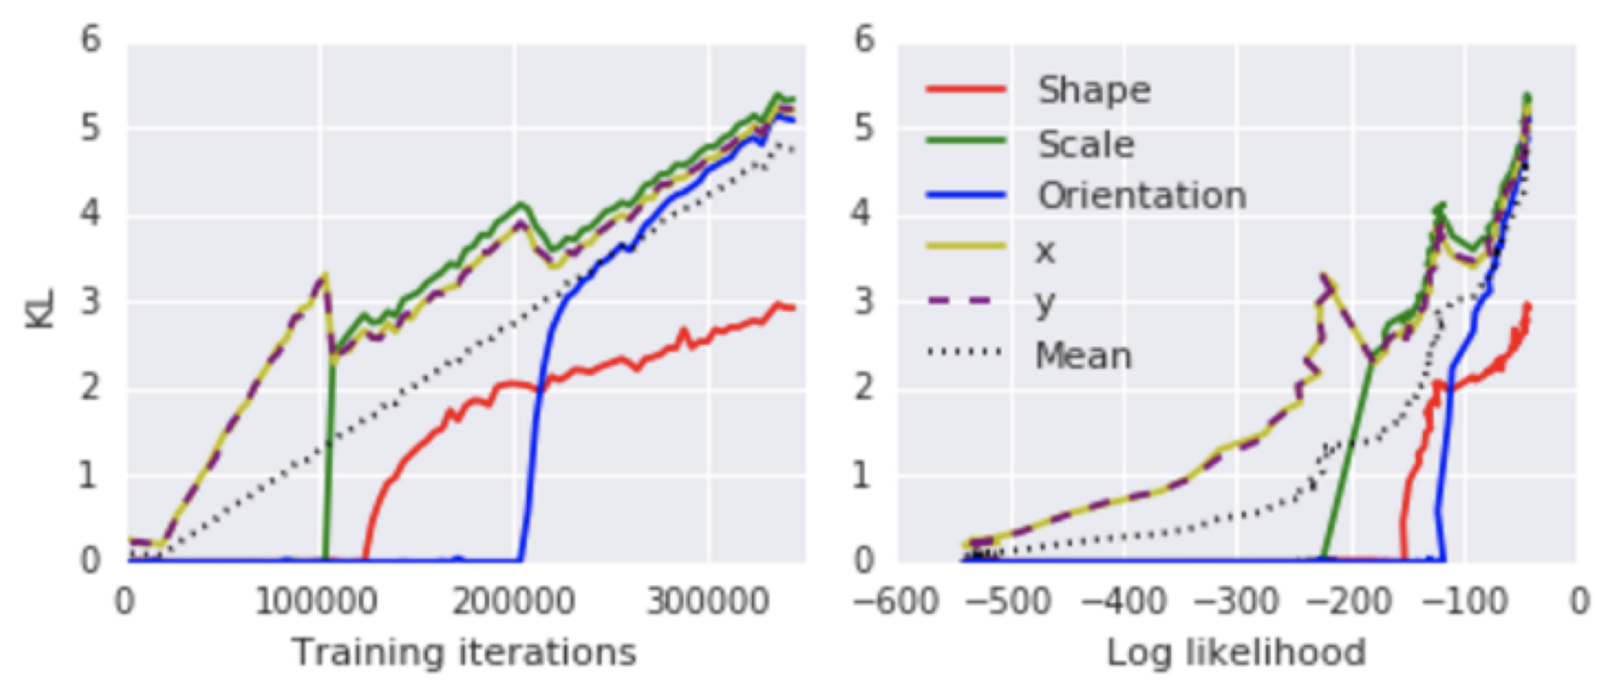
\includegraphics[width=0.9\linewidth]{figs/betaVAE_7.png}
	\end{figure}
	The early capacity is allocated to positional latents only, followed by a scale latent, then shape and orientation latents.
	
	\myfootnotewithlink{https://arxiv.org/abs/1804.03599}{Burgess C. P. et al. Understanding disentangling in $\beta$-VAE, 2018}
\end{frame}
%=======
\begin{frame}{$\beta$-VAE}
	\begin{block}{Controlled encoding capacity}
		\vspace{-0.5cm}
		\[
		\mathcal{L}(q, \btheta, \beta) = \mathbb{E}_{q(\bz | \bx)} \log p(\bx | \bz, \btheta) - | KL (q(\bz | \bx) || p(\bz)) - C|.
		\]
		\vspace{-0.5cm}
	\end{block}
	\begin{figure}
		\centering
		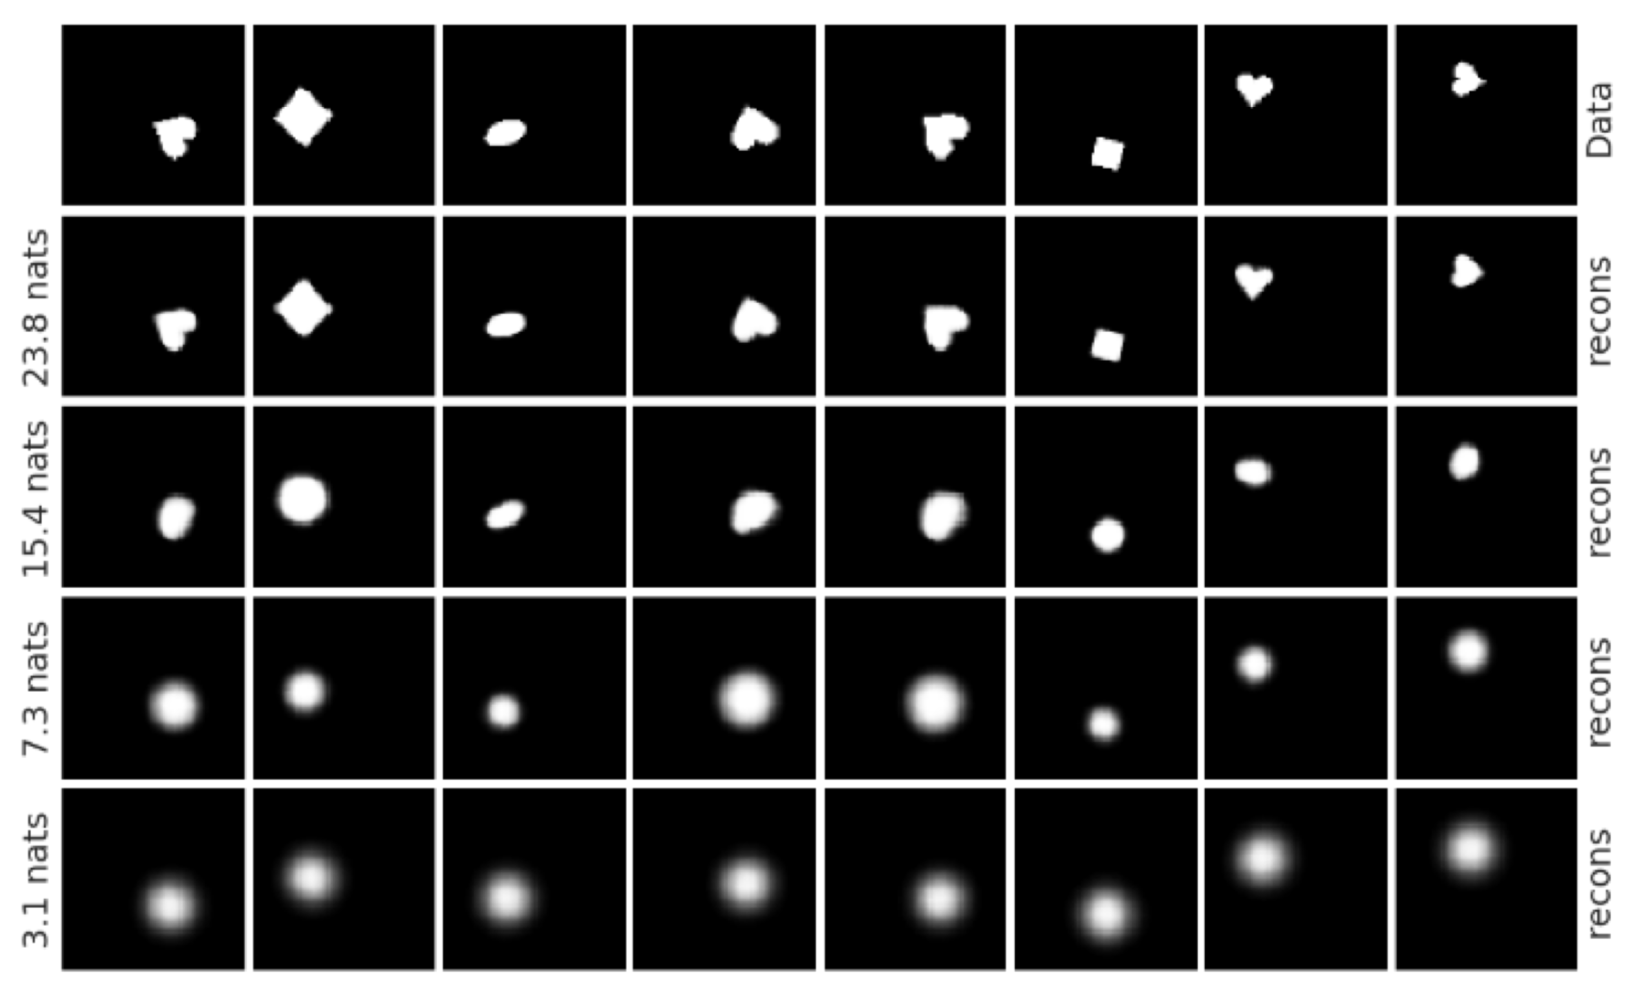
\includegraphics[width=0.7\linewidth]{figs/betaVAE_8.png}
	\end{figure}
	
	\myfootnotewithlink{https://arxiv.org/abs/1804.03599}{Burgess C. P. et al. Understanding disentangling in $\beta$-VAE, 2018}
\end{frame}
%=======
\begin{frame}{$\beta$-VAE}
	\begin{figure}
		\centering
		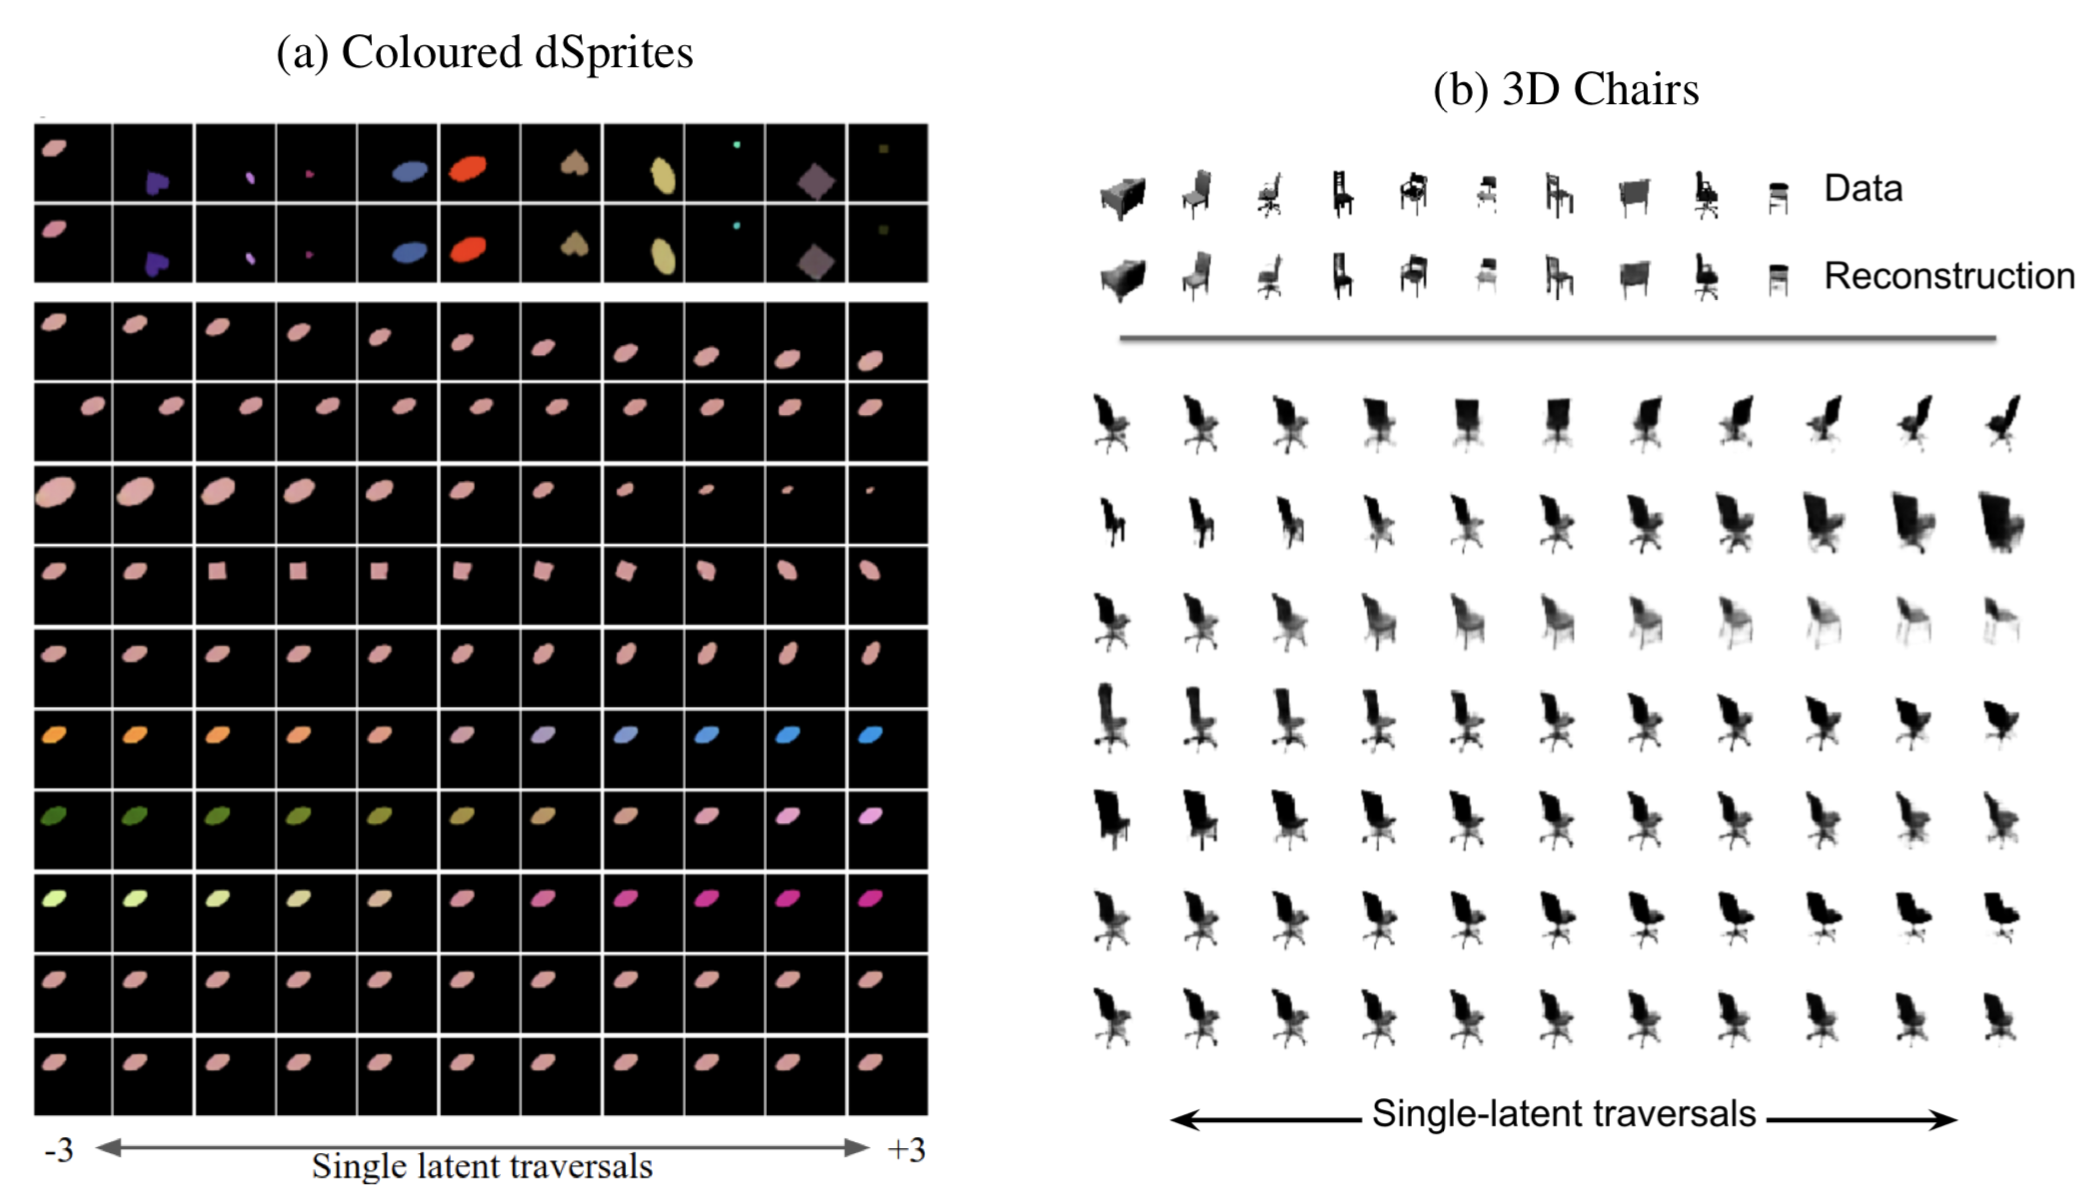
\includegraphics[width=1.0\linewidth]{figs/betaVAE_9.png}
	\end{figure}
	
	\myfootnotewithlink{https://arxiv.org/abs/1804.03599}{Burgess C. P. et al. Understanding disentangling in $\beta$-VAE, 2018}
\end{frame}
%=======
\subsection{FactorVAE}
%=======
\begin{frame}{FactorVAE}
	\begin{block}{Disentangled aggregated variational posterior}
		\vspace{-0.3cm}
		\[
			q(\bz) = \frac{1}{n} \sum_{i=1}^n q(\bz | \bx) = \prod_{j=1}^d q(z_j)
		\]
		\vspace{-0.3cm}
	\end{block}
	\begin{block}{Total correlation regularizer}
		\vspace{-0.3cm}
		\[
		\min KL(q(\bz) || \prod_{j=1}^d q(z_j))
		\]
		\vspace{-0.3cm}
	\end{block}
	\begin{block}{FactorVAE objective}
		\vspace{-0.3cm}
		\[
		\min_{\bphi, \btheta} \cL(\bphi, \btheta) - \gamma \cdot KL(q(\bz) || \prod_{j=1}^d q(z_j))
		\]
		\vspace{-0.3cm}
	\end{block}
	\begin{itemize}
		\item The last term is intractable.
		\item FactorVAE uses density ratio trick for estimation. 
	\end{itemize}

	\myfootnotewithlink{https://arxiv.org/abs/1802.05983}{Kim H., Mnih A. Disentangling by Factorising, 2018}
\end{frame}
%=======
\begin{frame}{FactorVAE}
	Consider two distributions $q_1(\bx)$, $q_2(\bx)$ and probilistic model
	\[
		p(\bx | y) = \begin{cases}
			q_1(\bx), \text{ if } y = 1, \\
			q_2(\bx), \text{ if } y = 0,
		\end{cases}
		\quad 
		y \sim \text{Bern}(0.5).
	\]
	\begin{block}{Density ratio trick}
		\vspace{-0.5cm}
		\begin{multline*}
			\frac{q_1(\bx)}{q_2(\bx)} = \frac{p(\bx | y = 1)}{p(\bx | y = 0)} = \frac{p(y = 1 | \bx) p(\bx)}{p(y=1)} \bigg/ \frac{p(y = 0 | \bx) p(\bx)}{p(y=0)} = \\
			= \frac{p(y = 1 | \bx)}{p(y = 0 | \bx)} = \frac{p(y = 1 | \bx)}{1 - p(y = 1 | \bx)} = \frac{D(\bx)}{1 - D(\bx)}
		\end{multline*}
	Here $D(\bx)$ could be treated as a discriminator a model the output of which is a probability that $\bx$ is a sample
	from $q_1(\bx)$ rather than from $q_2(\bx)$.
	\end{block}

	\myfootnotewithlink{https://arxiv.org/abs/1802.05983}{Kim H., Mnih A. Disentangling by Factorising, 2018}
\end{frame}
%=======
\begin{frame}{FactorVAE}
	
	\begin{block}{FactorVAE objective}
		\vspace{-0.3cm}
		\[
		\min_{\btheta, \bphi} \text{ELBO}(\btheta, \bphi) - \gamma \cdot KL(q(\bz) || \prod_{j=1}^d q(z_j))
		\]
		\vspace{-0.3cm}
	\end{block}
	
	\begin{block}{Total correlation regularizer}
		\vspace{-0.7cm}
		\begin{multline*}
		KL(q(\bz) || \prod_{j=1}^d q(z_j)) = KL(q(\bz) || \bar{q}(\bz)) = \\ =\bbE_{q(\bz)} \log \frac{q(\bz)}{\bar{q}(\bz)} \approx \bbE_{q(\bz)} \log \frac{D(\bz)}{1 - D(\bz)}
		\end{multline*}
		\vspace{-0.3cm}
	\end{block}
	VAE and GAN are trained simultaneously.

	\myfootnotewithlink{https://arxiv.org/abs/1802.05983}{Kim H., Mnih A. Disentangling by Factorising, 2018}
\end{frame}
%=======
\begin{frame}{FactorVAE}
	
	\begin{minipage}[t]{0.5\columnwidth}
		\begin{figure}
			\centering
			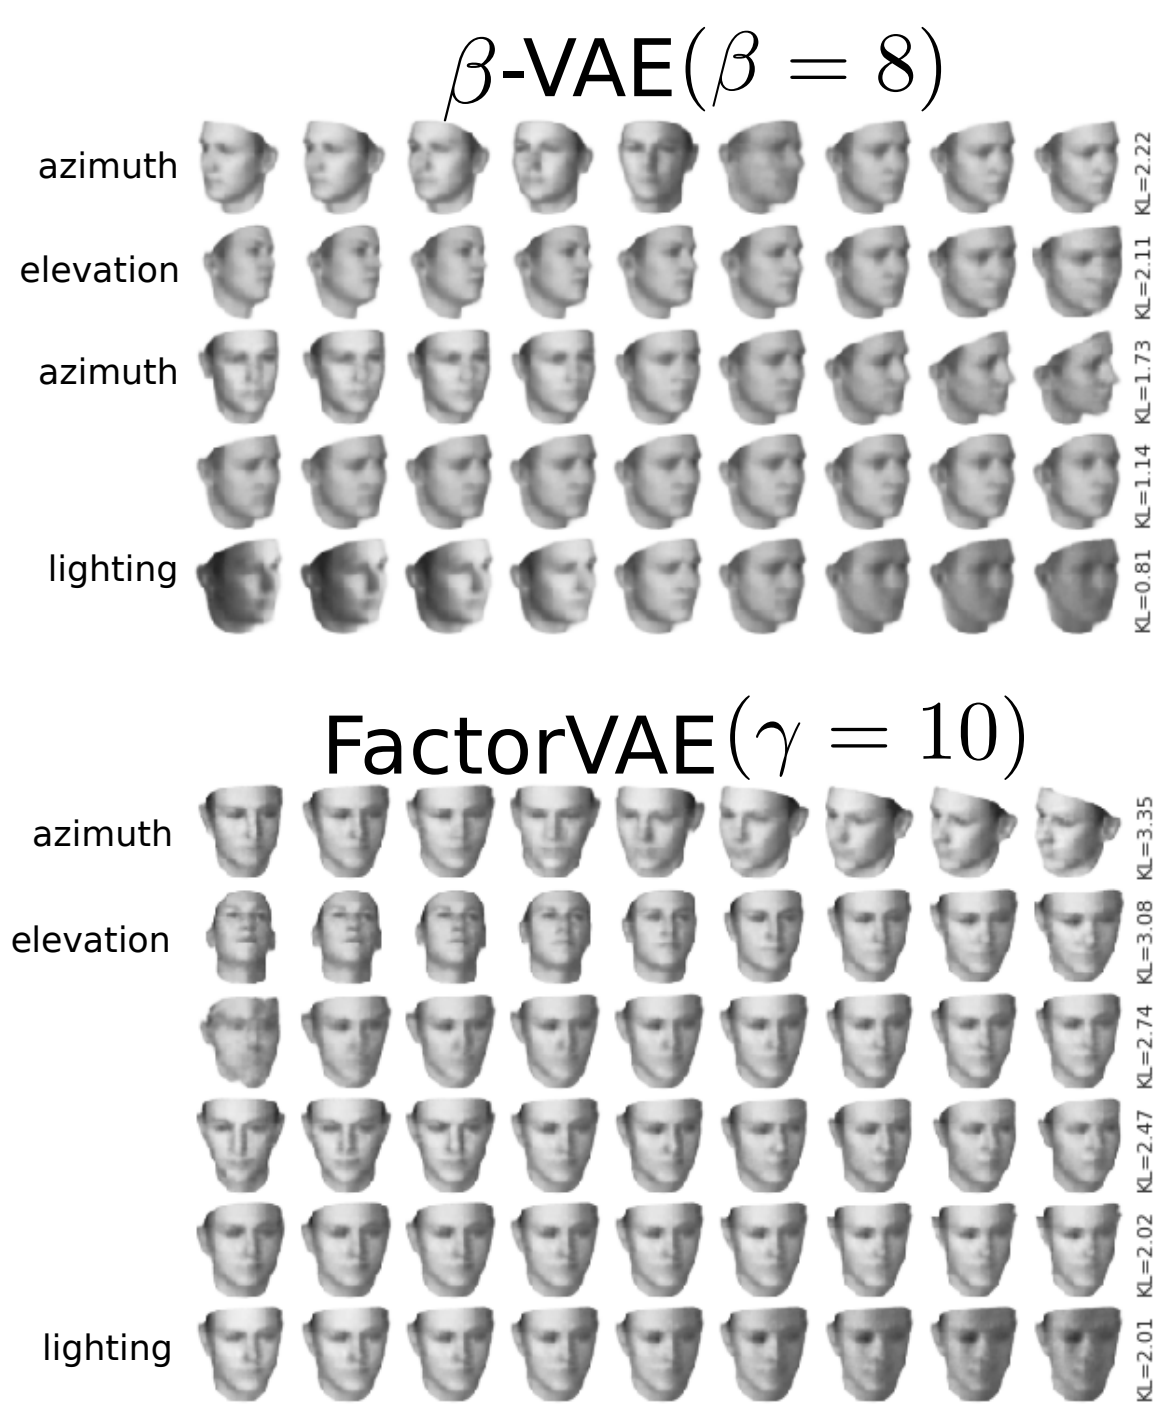
\includegraphics[width=\linewidth]{figs/factorvae_1}
		\end{figure}
	\end{minipage}%
	\begin{minipage}[t]{0.5\columnwidth}
		\vspace{1.7cm}
		\begin{figure}[h]
			\centering
			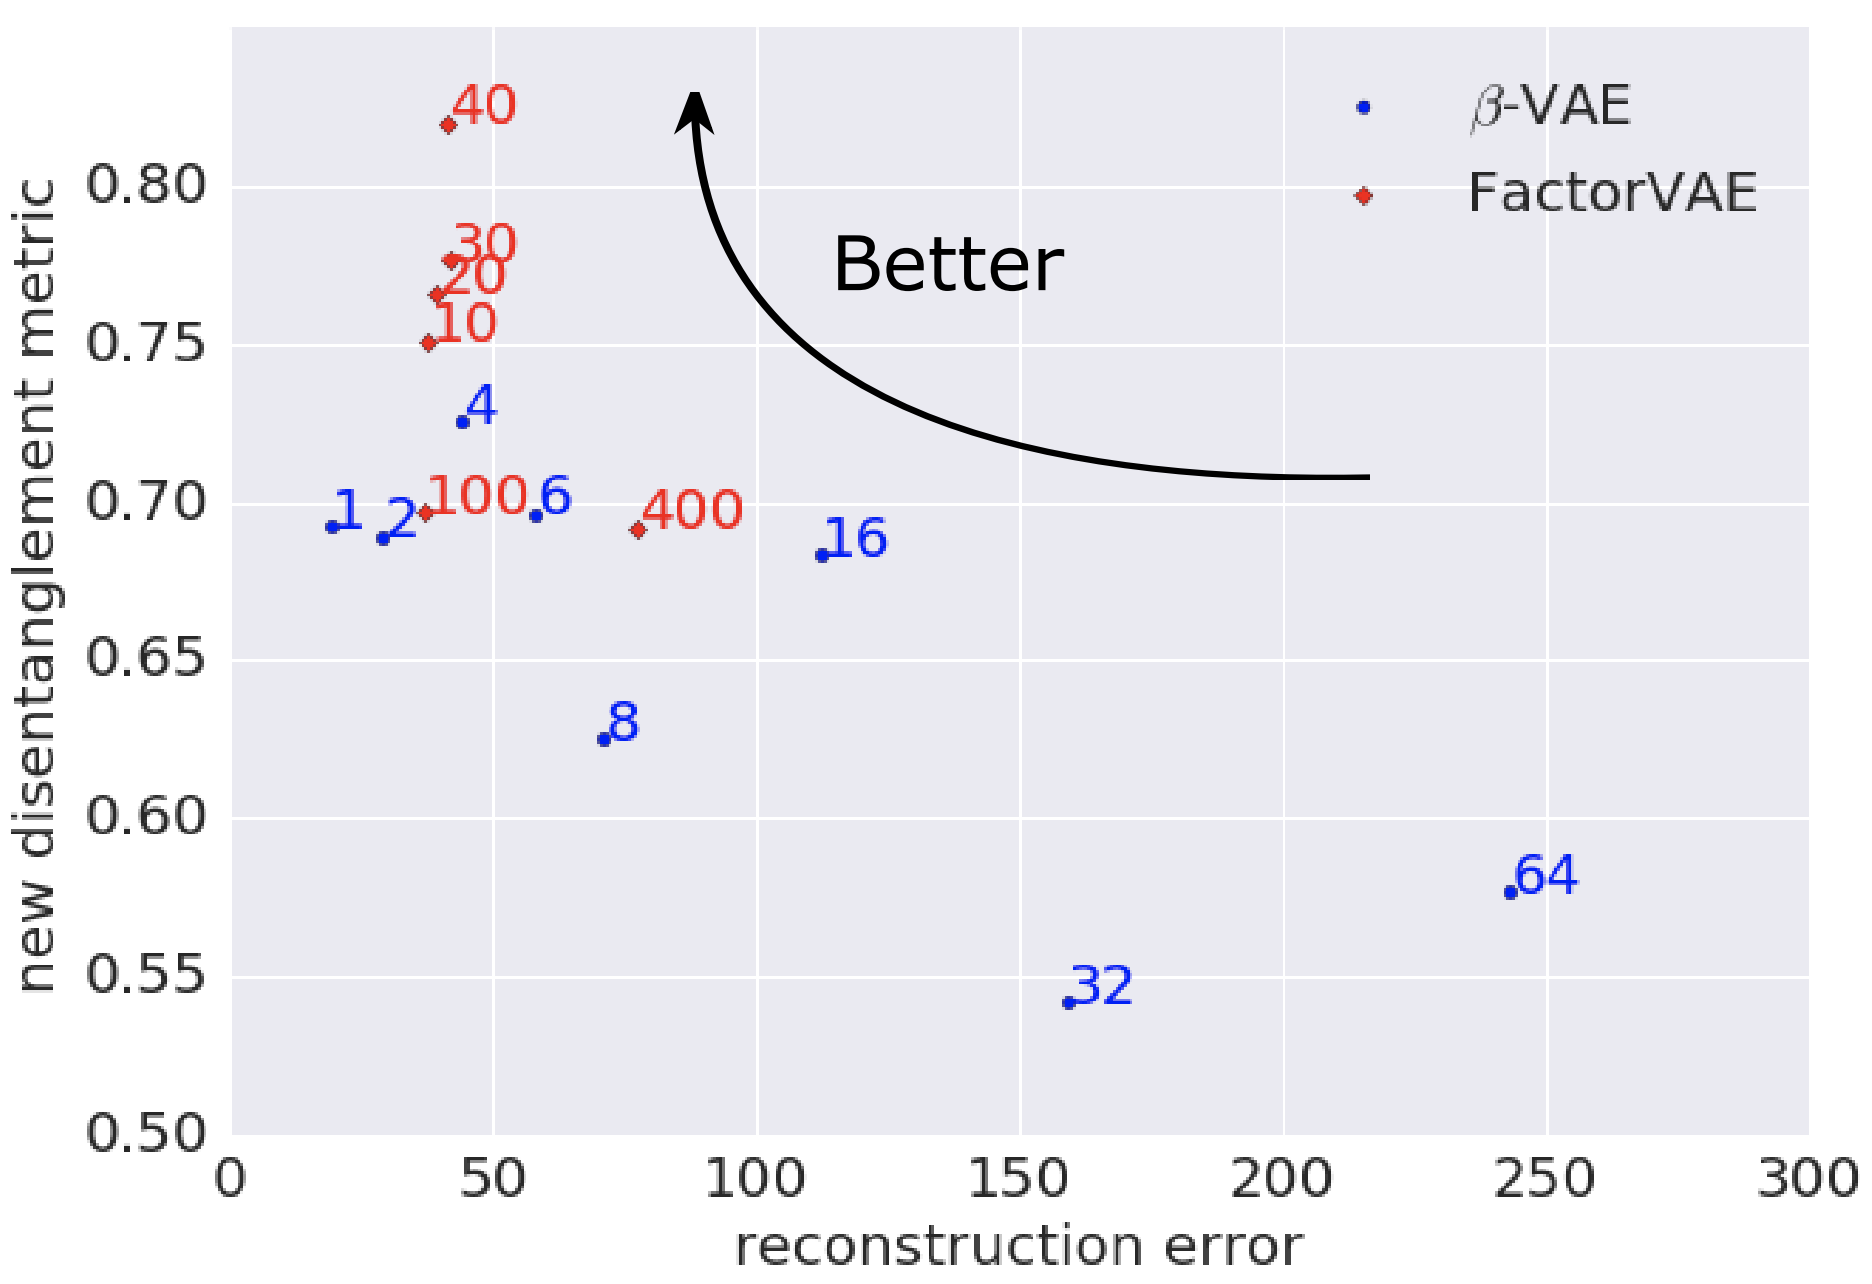
\includegraphics[width=\linewidth]{figs/factorvae_2}
		\end{figure}
	\end{minipage}

	\myfootnotewithlink{https://arxiv.org/abs/1802.05983}{Kim H., Mnih A. Disentangling by Factorising, 2018}
\end{frame}
%=======
\subsection{Challenging Disentanglement Assumptions}
%=======
\begin{frame}{Challenging Disentanglement Assumptions}
\begin{block}{Proof (1)}
	\begin{enumerate}
		\item 
		Consider the function $g: \text{supp}(\bz) \rightarrow [0, 1]^d$:
		\vspace{-0.1cm}
		\[
		g_i(\bu) = P(z_i \leq u_i), \quad i=1, \dots, d.
		\]
		\vspace{-0.4cm}
		\begin{itemize}
			\item $g$ is bijective (since $p(\bz) = \prod_{i=1}^dp(z_i)$).
			\item $\frac{\partial g_i(\bu)}{\partial u_i} \neq 0$, for all $i$ and $\frac{\partial g_i(\bu)}{\partial u_j} = 0$ for all $i \neq j$.
			\item $g(\bz)$ is an independent $d$-dimensional uniform distribution.
		\end{itemize}
		\item 
		Consider $h: (0, 1]^d \rightarrow \bbR^d$
		\[
		h_i(\bu) = \psi^{-1}(u_i), \quad i= 1, \dots, d.
		\]
		Here $\psi$  denotes the CDF of a standard normal distribution.
		\begin{itemize}
			\item $h$ is bijective.
			\item $\frac{\partial h_i(\bu)}{\partial u_i} \neq 0$, for all $i$ and $\frac{\partial h_i(\bu)}{\partial u_j} = 0$ for all $i \neq j$.
			\item $h(g(\bz))$  is a $d$-dimensional standard normal distribution.
		\end{itemize}
	\end{enumerate}
\end{block}

\myfootnotewithlink{https://arxiv.org/abs/1811.12359}{Locatello F. et al. Challenging Common Assumptions in the Unsupervised Learning of Disentangled Representations, 2018}
\end{frame}
%=======
\begin{frame}{Challenging Disentanglement Assumptions}
\begin{block}{Proof (2)}
	Let $\bA \in \bbR^{d \times d}$ be an arbitrary orthogonal matrix with $A_{ij} \neq 0$ for all $i, j$.
	The family of such matrices is infinite.
	\begin{itemize}
		\item $\bA$ is orthogonal, it is invertible and thus defines a bijective linear operator. 
		\item $\bA h(g(\bz)) \in \bbR^d$ is hence an independent, multivariate standard normal distribution.
		\item $h^{-1}( \bA h(g(\bz))) \in \bbR^d$ is an independent $d$-dimensional uniform distribution.
	\end{itemize}
	Define $f: \text{supp}(\bz) \rightarrow \text{supp}(\bz)$:
	\vspace{-0.2cm}
	\[
	f(\bu) = g^{-1} (h^{-1}( \bA h(g(\bz)))).
	\]
	By definition $f(\bz)$ has the same marginal distribution as $\bz$: $P(\bz \leq \bu) = P(f(\bz) \leq \bu)$ and $\frac{\partial f_i(\bz)}{\partial z_j} \neq 0$.
\end{block}

\myfootnotewithlink{https://arxiv.org/abs/1811.12359}{Locatello F. et al. Challenging Common Assumptions in the Unsupervised Learning of Disentangled Representations, 2018}
\end{frame}
%=======
\begin{frame}{Challenging disentanglement assumptions}
	\begin{figure}
		\centering
		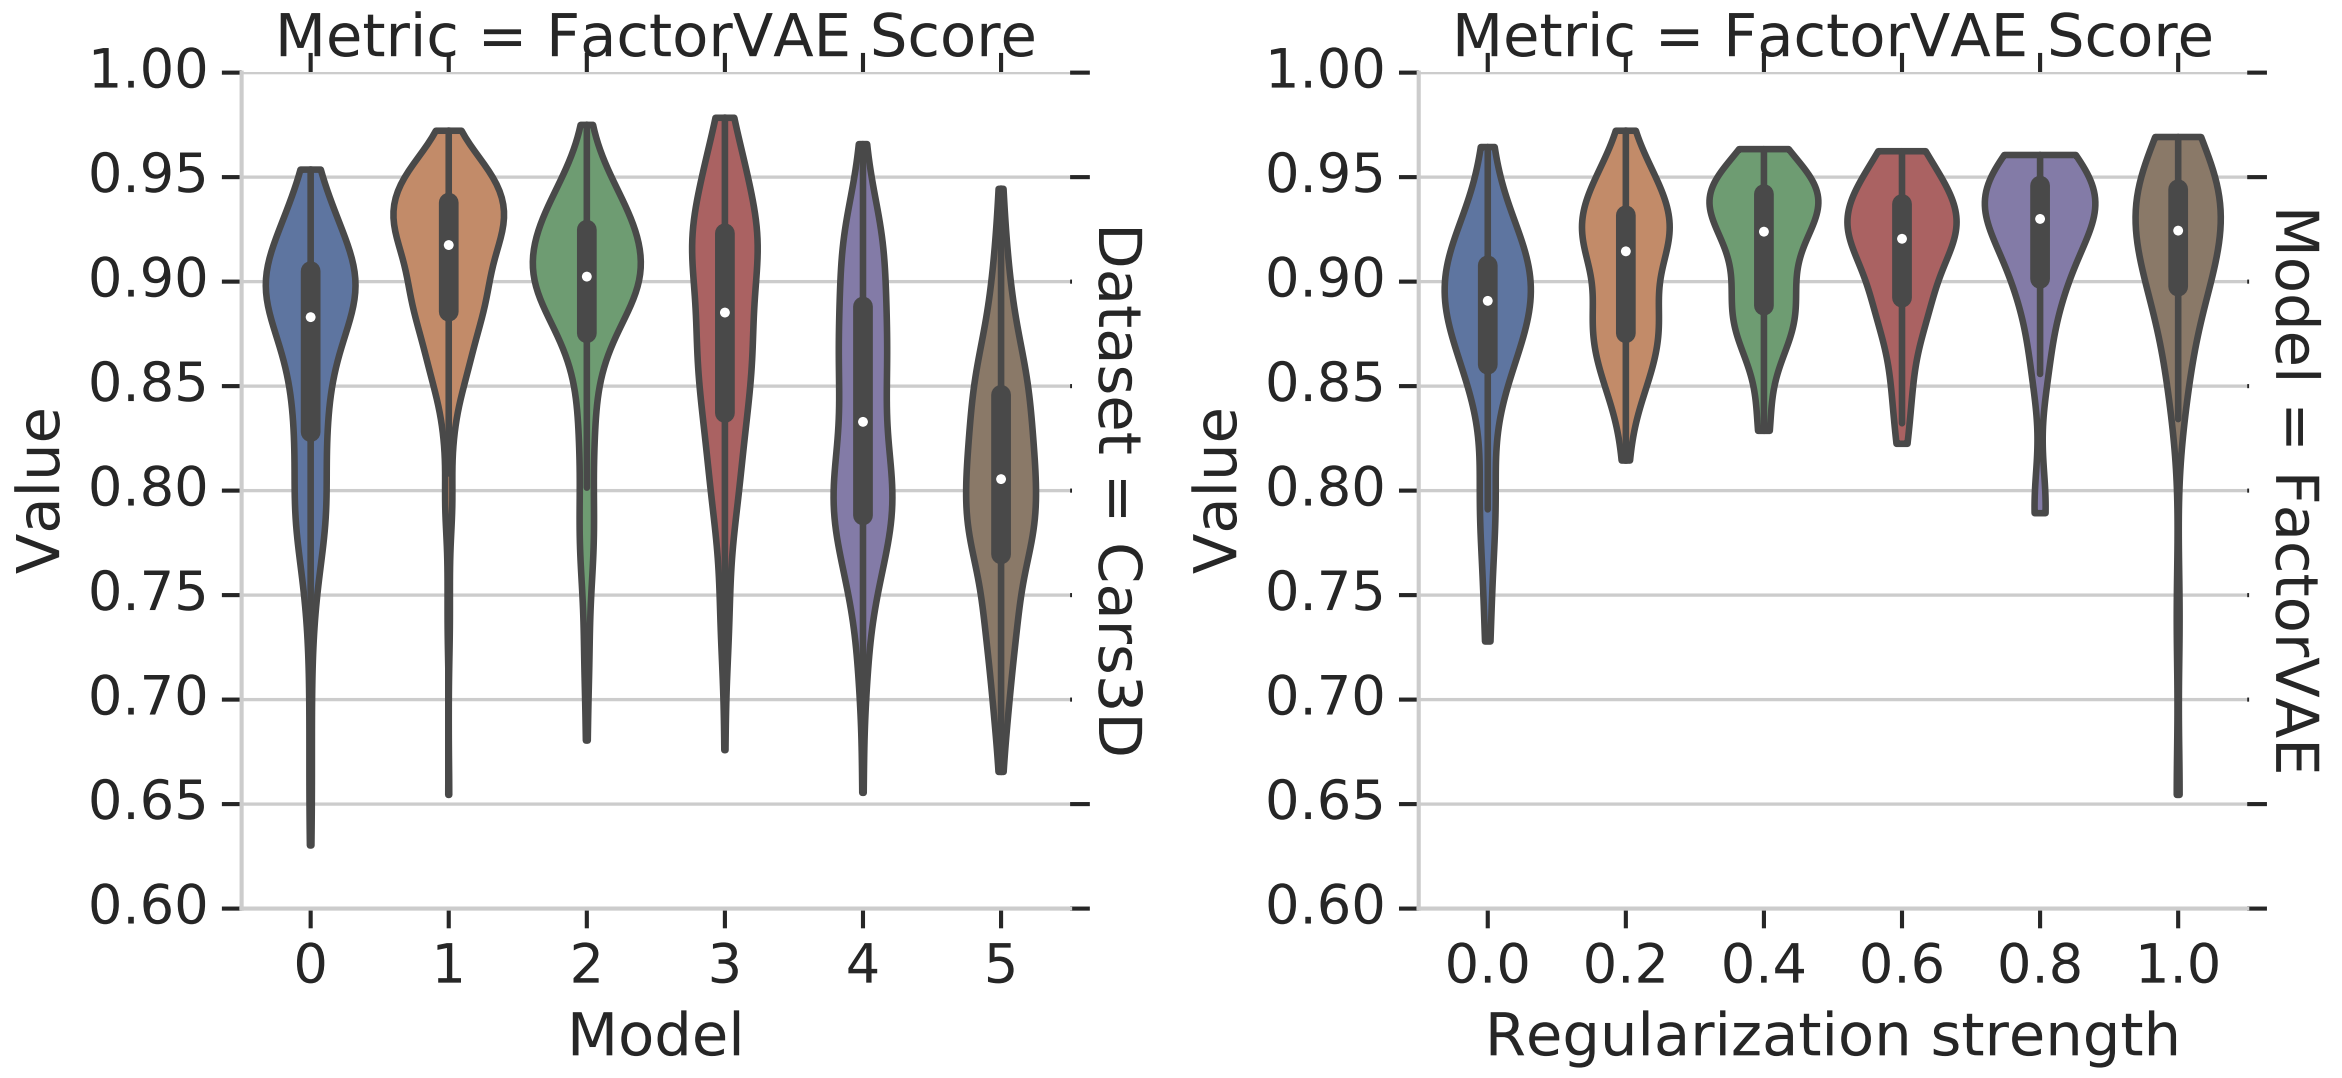
\includegraphics[width=0.85\linewidth]{figs/challenge_dis_2}
	\end{figure}
	\vspace{-0.3cm}
	\begin{figure}
		\centering
		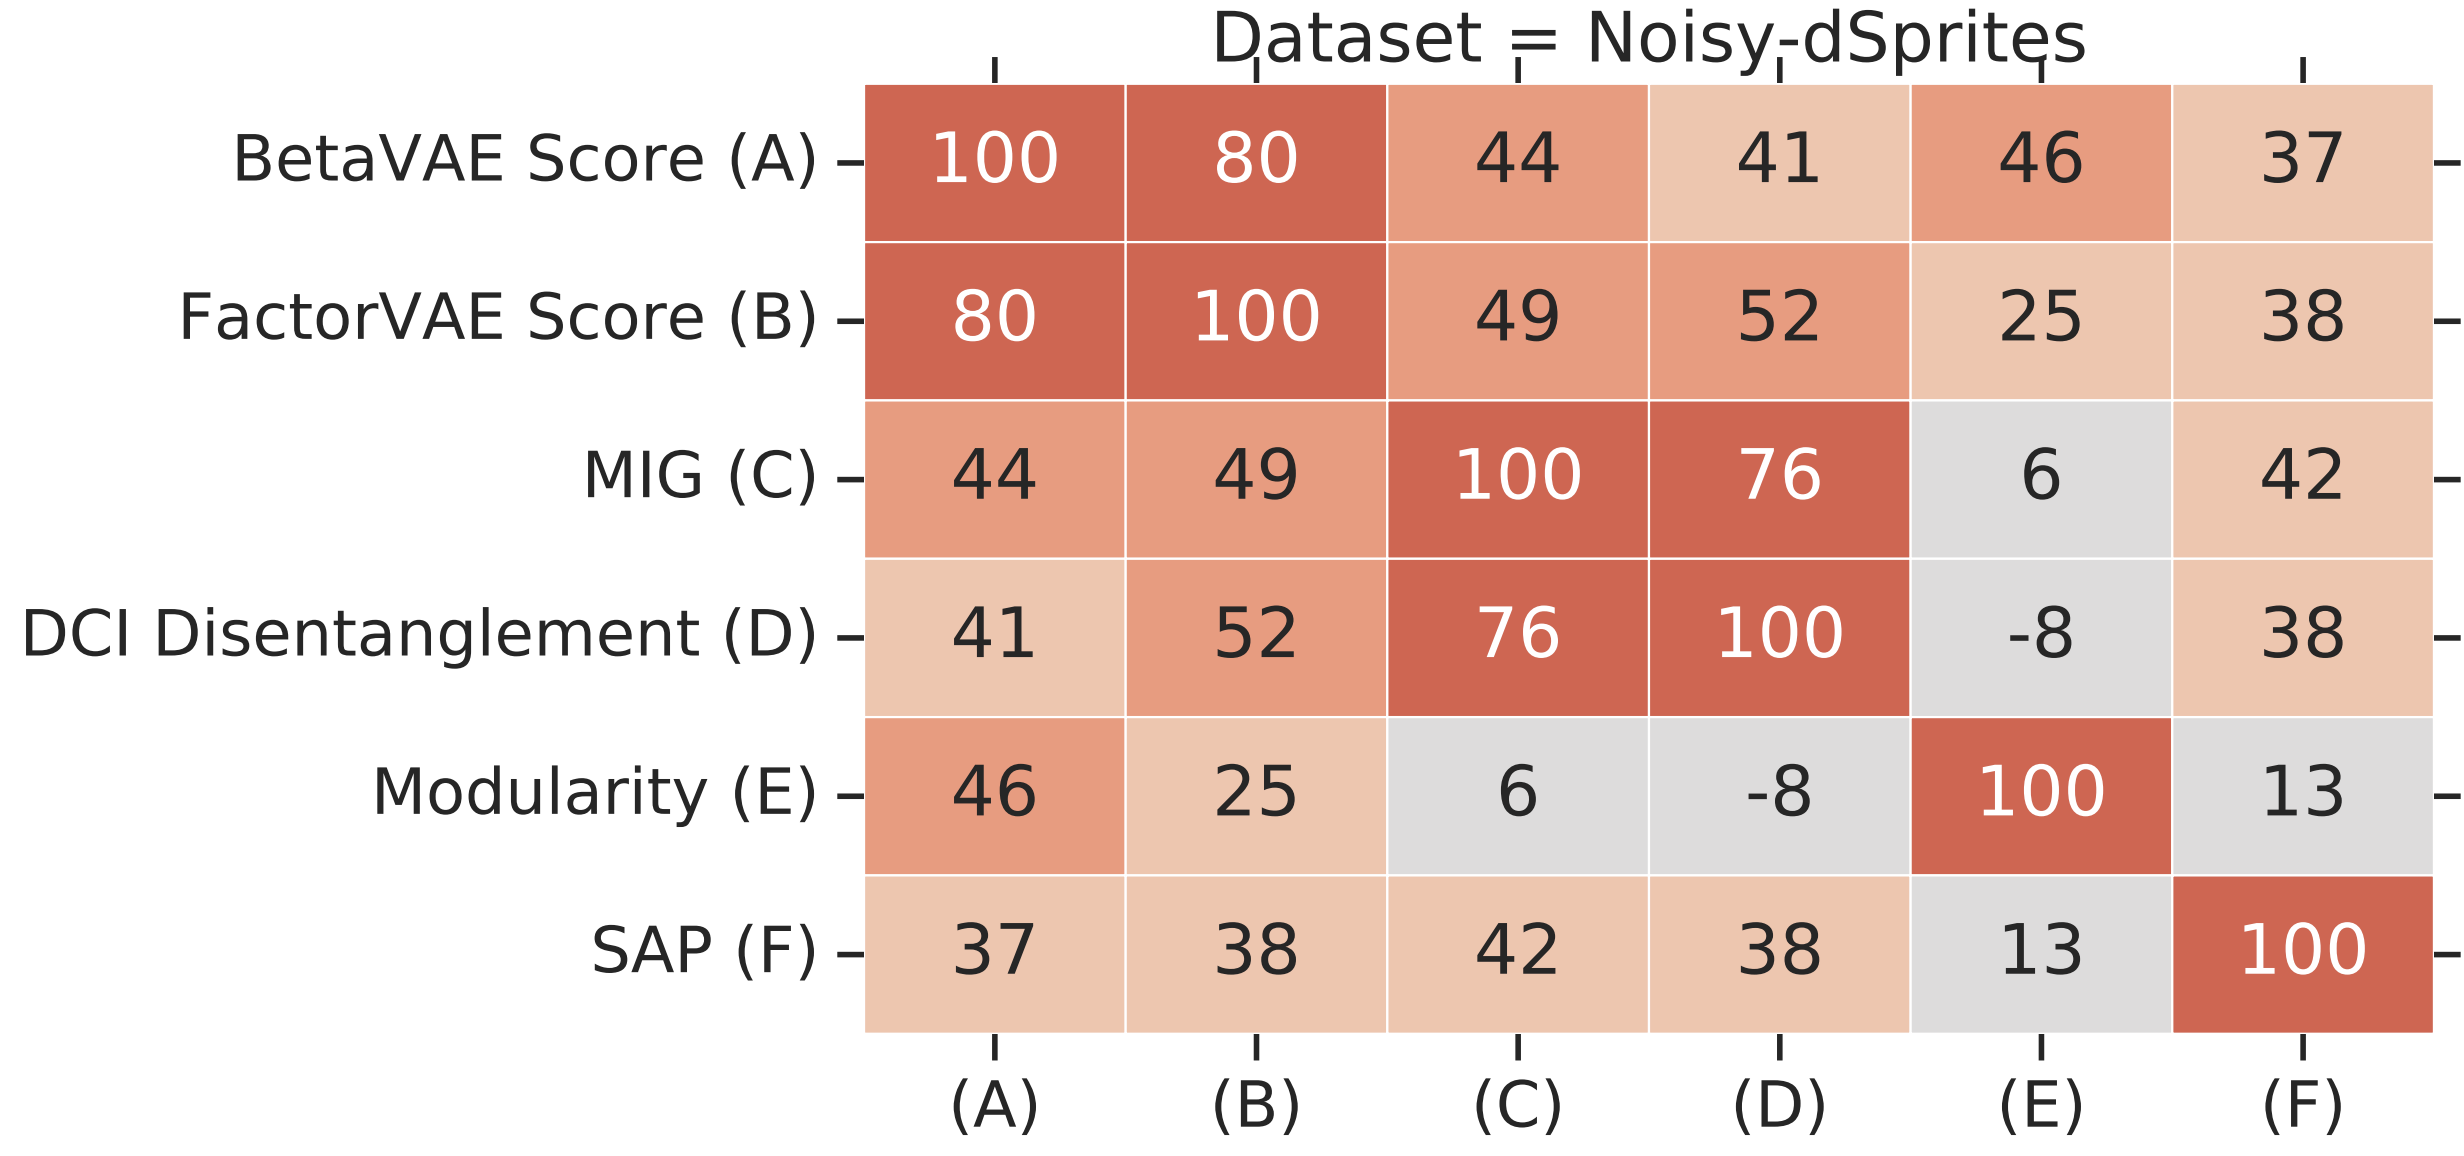
\includegraphics[width=0.65\linewidth]{figs/challenge_dis_3}
	\end{figure}

\myfootnotewithlink{https://arxiv.org/abs/1811.12359}{Locatello F. et al. Challenging Common Assumptions in the Unsupervised Learning of Disentangled Representations, 2018}
\end{frame}
%=======
\section{GANs}
%=======
\subsection{DCGAN}
%=======
\begin{frame}{Vanilla GAN results}
	\begin{figure}
		\centering
		\includegraphics[width=0.95\linewidth]{figs/Vanila_gan_results}
	\end{figure}
	\myfootnotewithlink{https://arxiv.org/abs/1406.2661}{Goodfellow I. J. et al. Generative Adversarial Networks, 2014}
\end{frame}
%=======
\begin{frame}{Deep Convolutional GAN}
	\begin{block}{Architecture}
		\vspace{-0.3cm}
		\begin{figure}
			\centering
			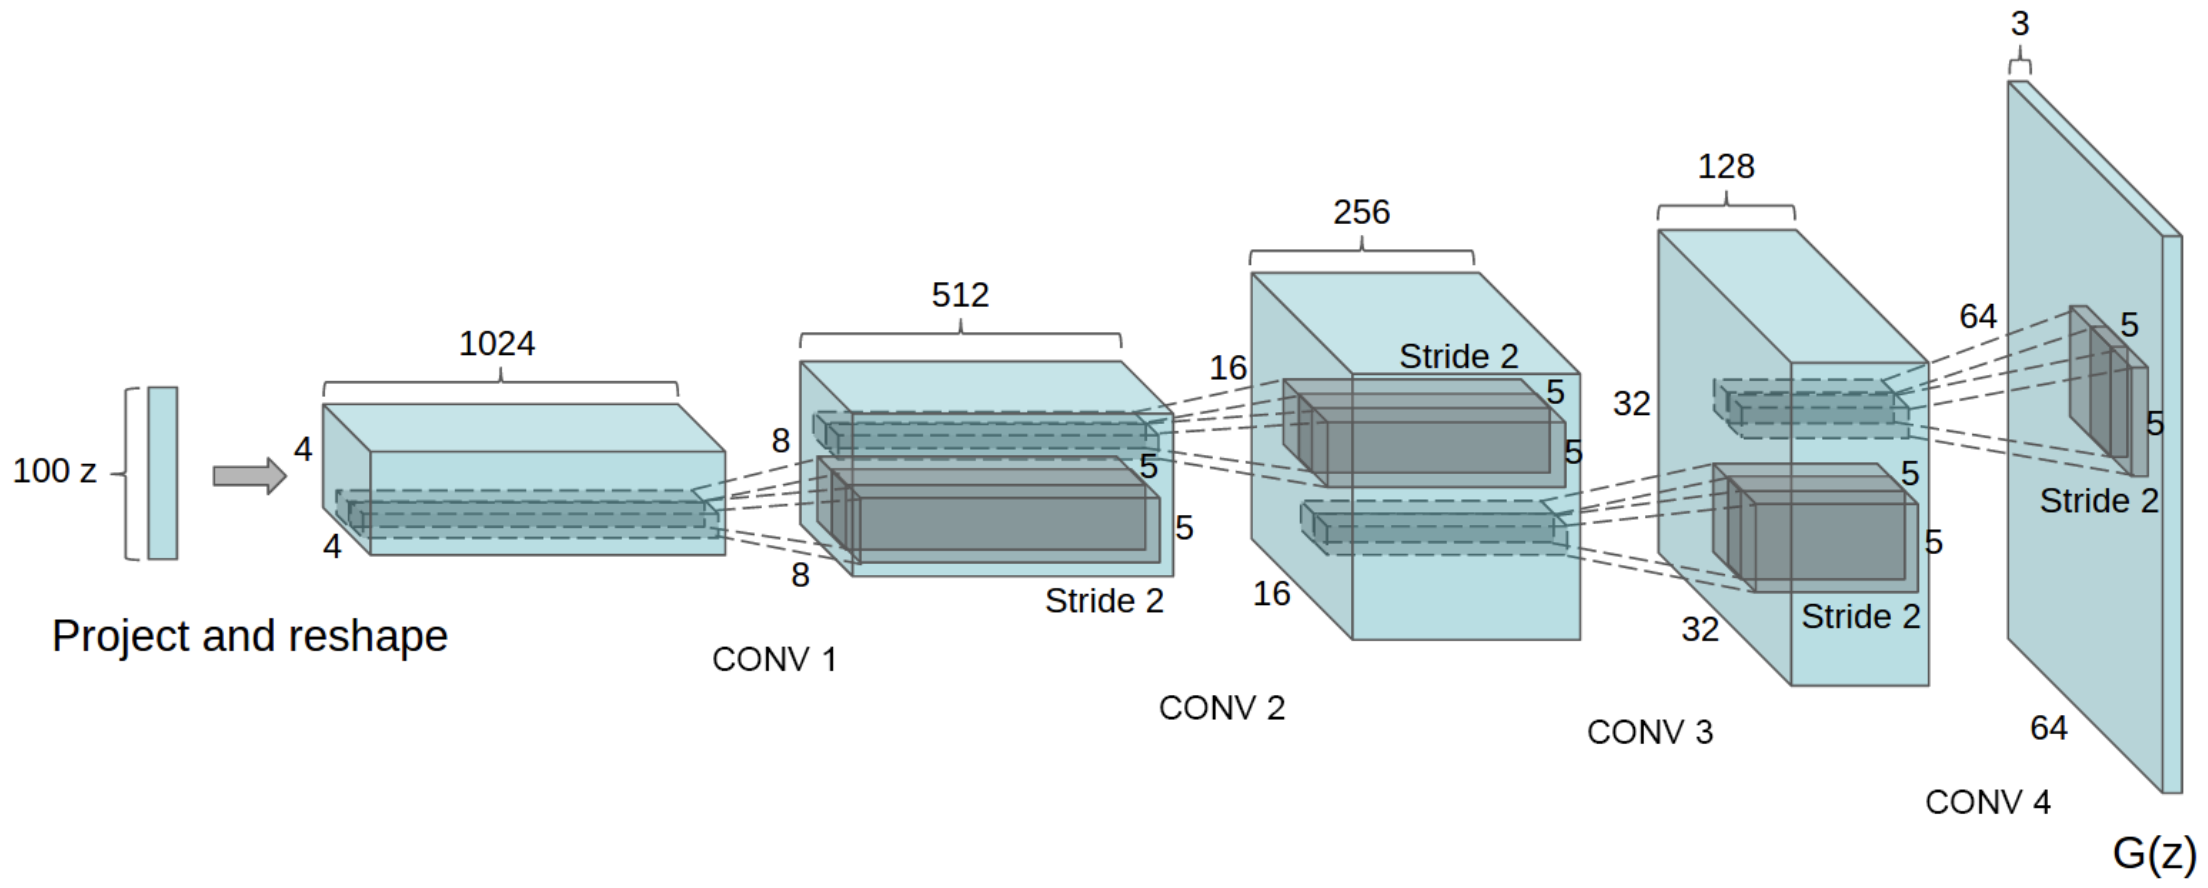
\includegraphics[width=0.8\linewidth]{figs/dcgan_1}
		\end{figure}
	\end{block}
	\vspace{-0.4cm}
	\begin{itemize}
		\footnotesize
		\item  Mean-pooling instead of max-pooling.
		\item Transposed convolutions in the generator for upsampling.
		\item Downsample with strided convolutions and average pooling.
		\item ReLU for generator, Leaky-ReLU (0.2) for discriminator.
		\item Output nonlinearity: tanh for Generator, sigmoid for discriminator.
		\item Batch Normalization used to prevent mode collapse (not applied at the output of $G$ and input of $D$).
		\item Adam: small LR = 2e-4; small momentum: 0.5, batch-size: 128.
	\end{itemize}
	\myfootnotewithlink{https://arxiv.org/abs/1511.06434}{Radford A., Metz L., Chintala S. Unsupervised Representation Learning with Deep Convolutional Generative Adversarial Networks, 2015}
\end{frame}
%=======
\begin{frame}{Deep Convolutional GAN}
	\begin{block}{ImageNet samples}
		\begin{figure}
			\centering
			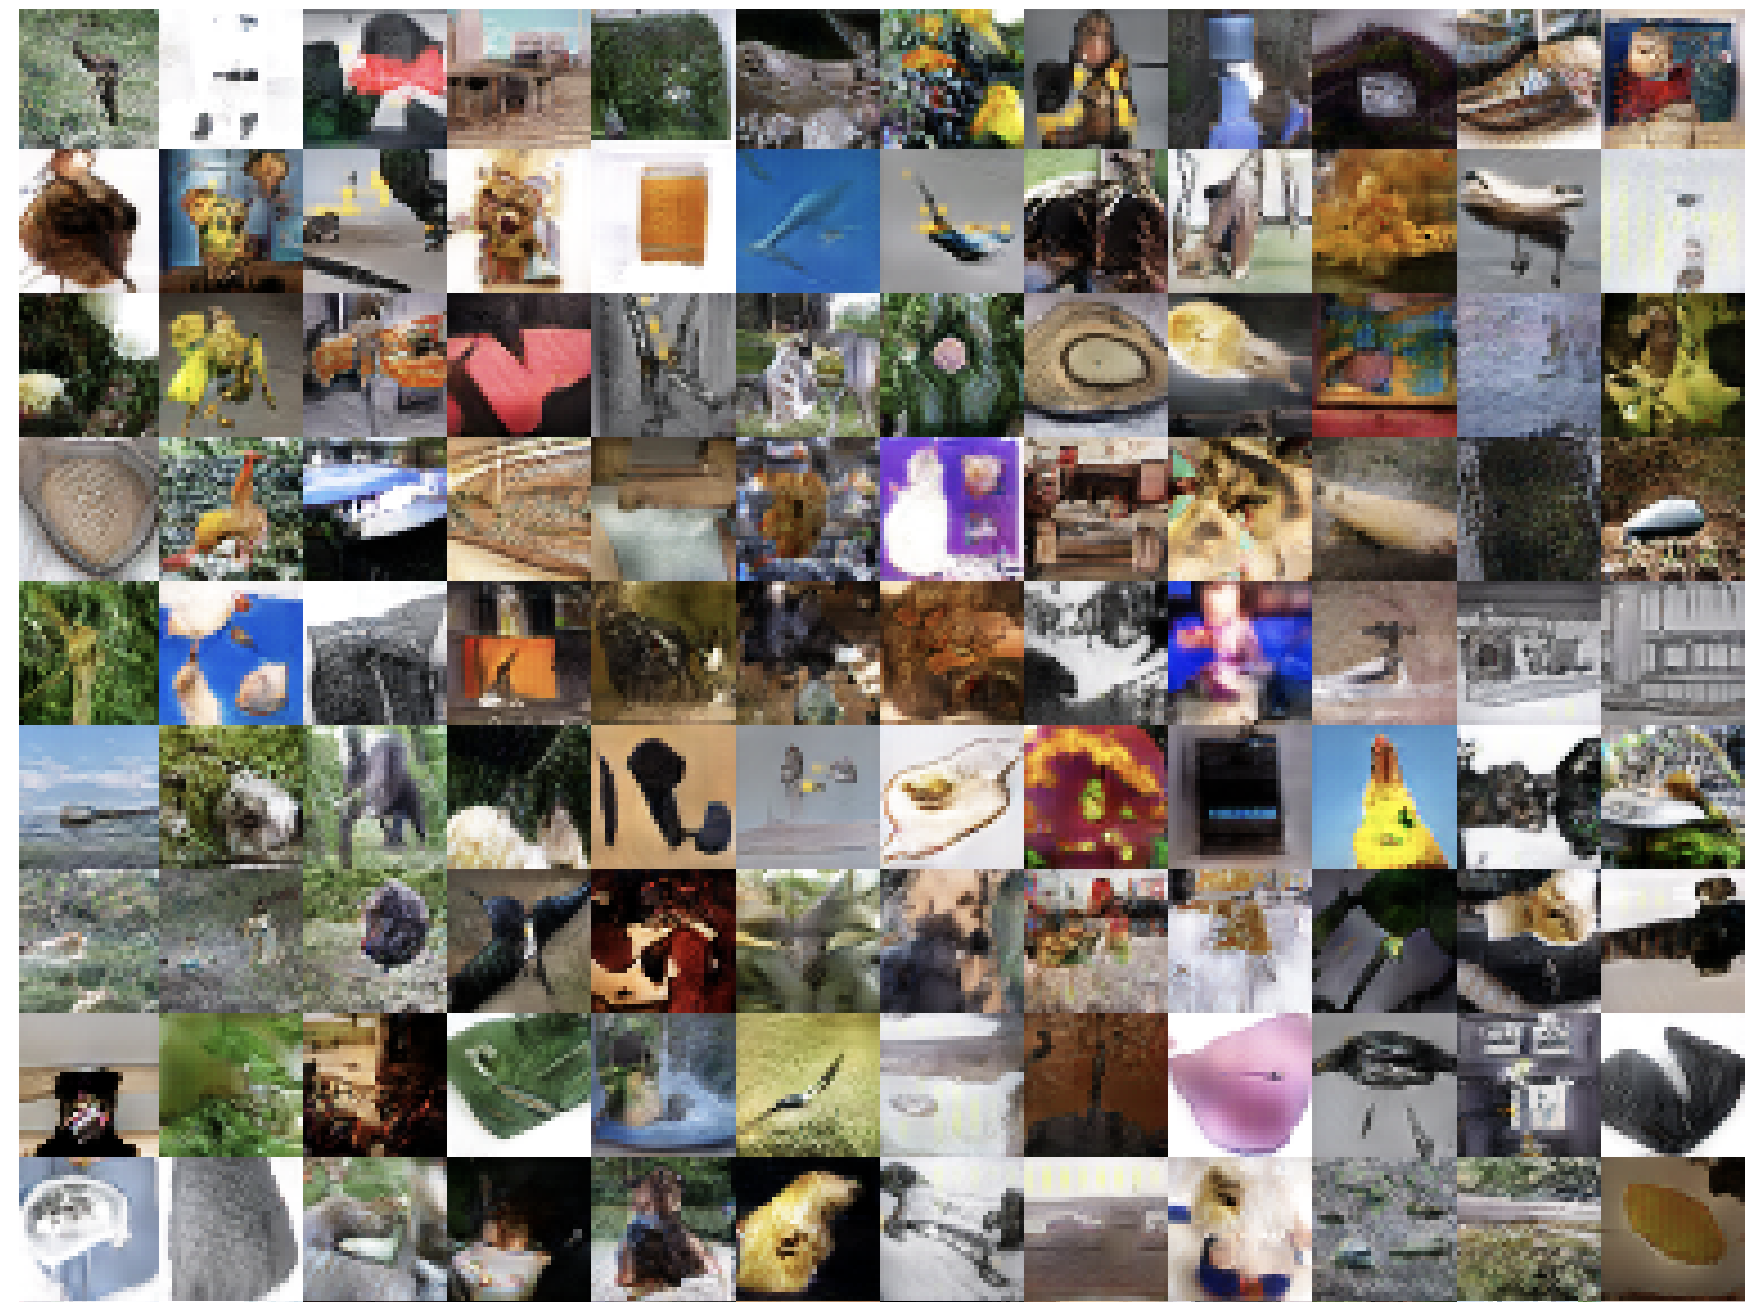
\includegraphics[width=0.8\linewidth]{figs/dcgan_results_1}
		\end{figure}
	\end{block}
	\myfootnotewithlink{https://arxiv.org/abs/1511.06434}{Radford A., Metz L., Chintala S. Unsupervised Representation Learning with Deep Convolutional Generative Adversarial Networks, 2015}
\end{frame}
%=======
\begin{frame}{Deep Convolutional GAN}
	\begin{block}{Smooth interpolations}
		\begin{figure}
			\centering
			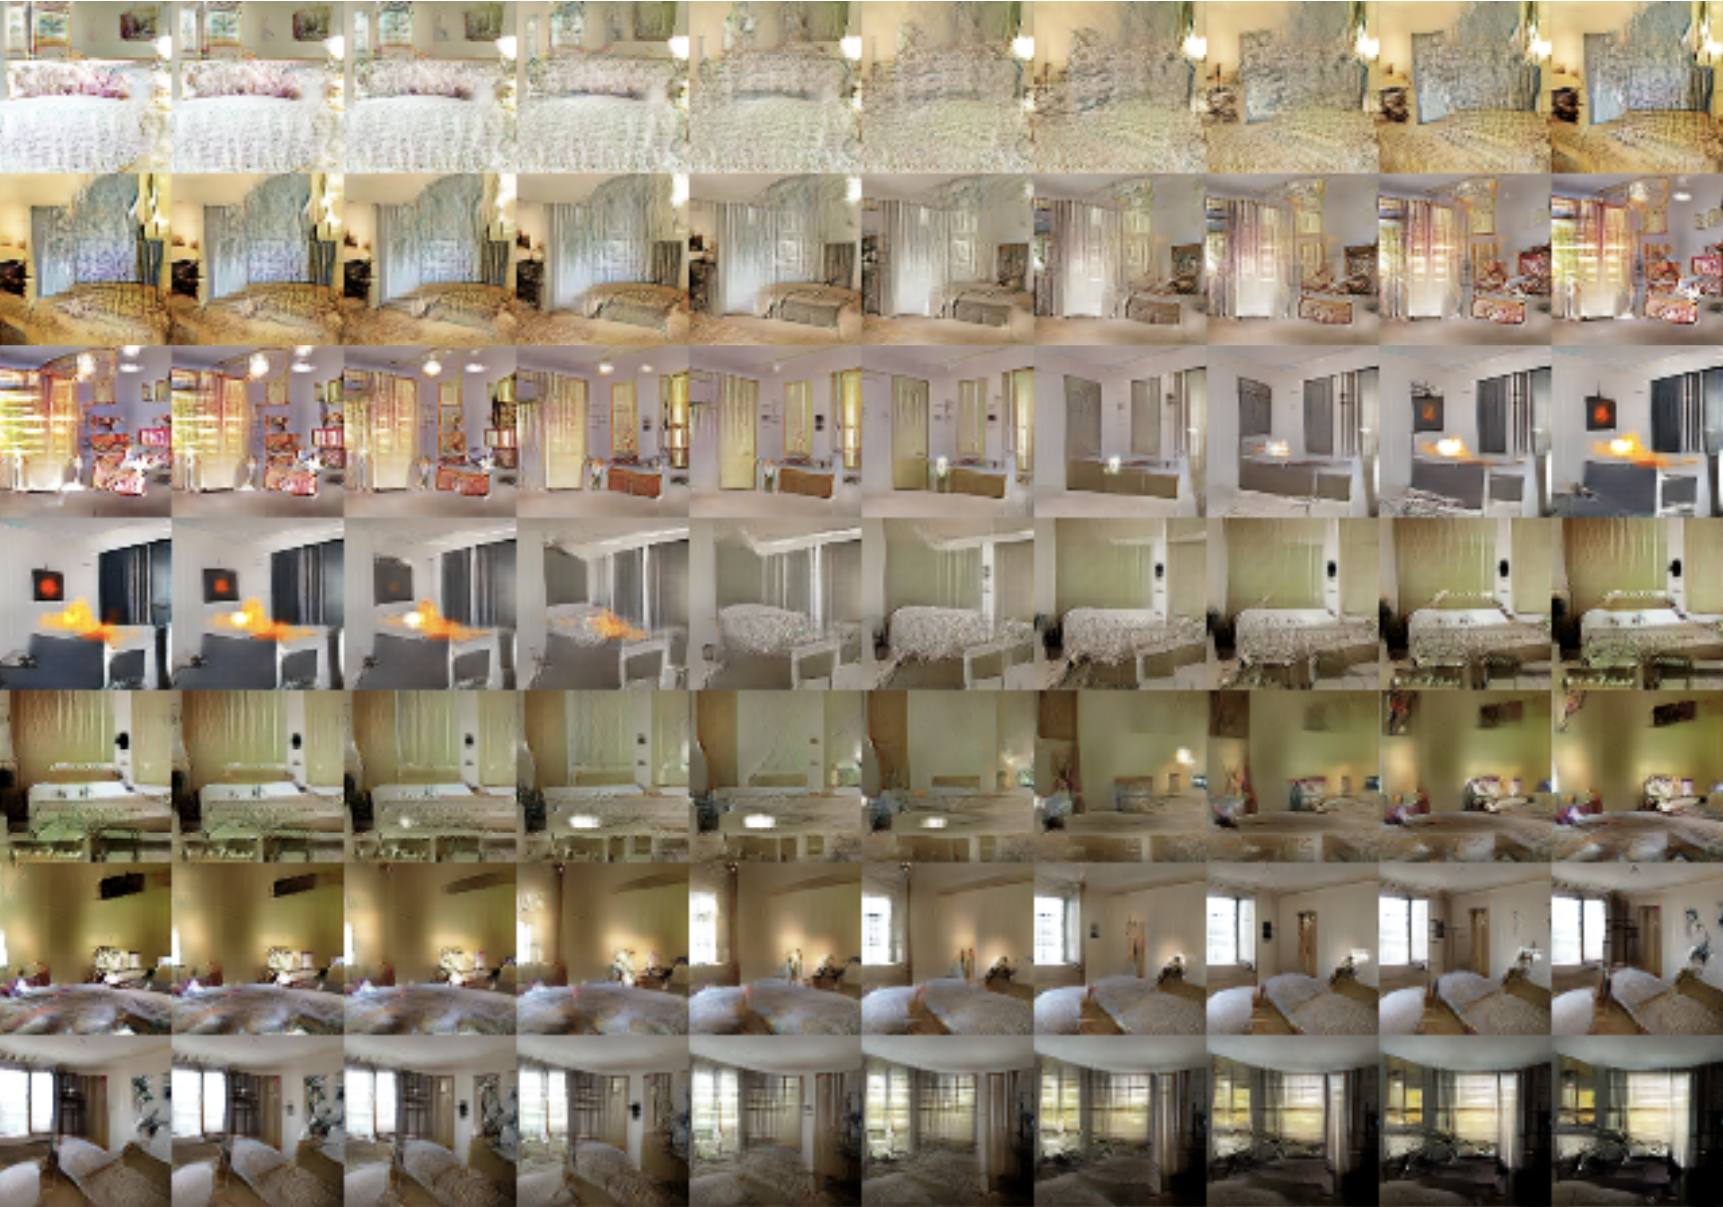
\includegraphics[width=0.8\linewidth]{figs/dcgan_results_2}
		\end{figure}
	\end{block}

	\myfootnotewithlink{https://arxiv.org/abs/1511.06434}{Radford A., Metz L., Chintala S. Unsupervised Representation Learning with Deep Convolutional Generative Adversarial Networks, 2015}
\end{frame}
%=======
\begin{frame}{Deep Convolutional GAN}
	\begin{block}{Vector arithmetic}
		\begin{figure}
			\centering
			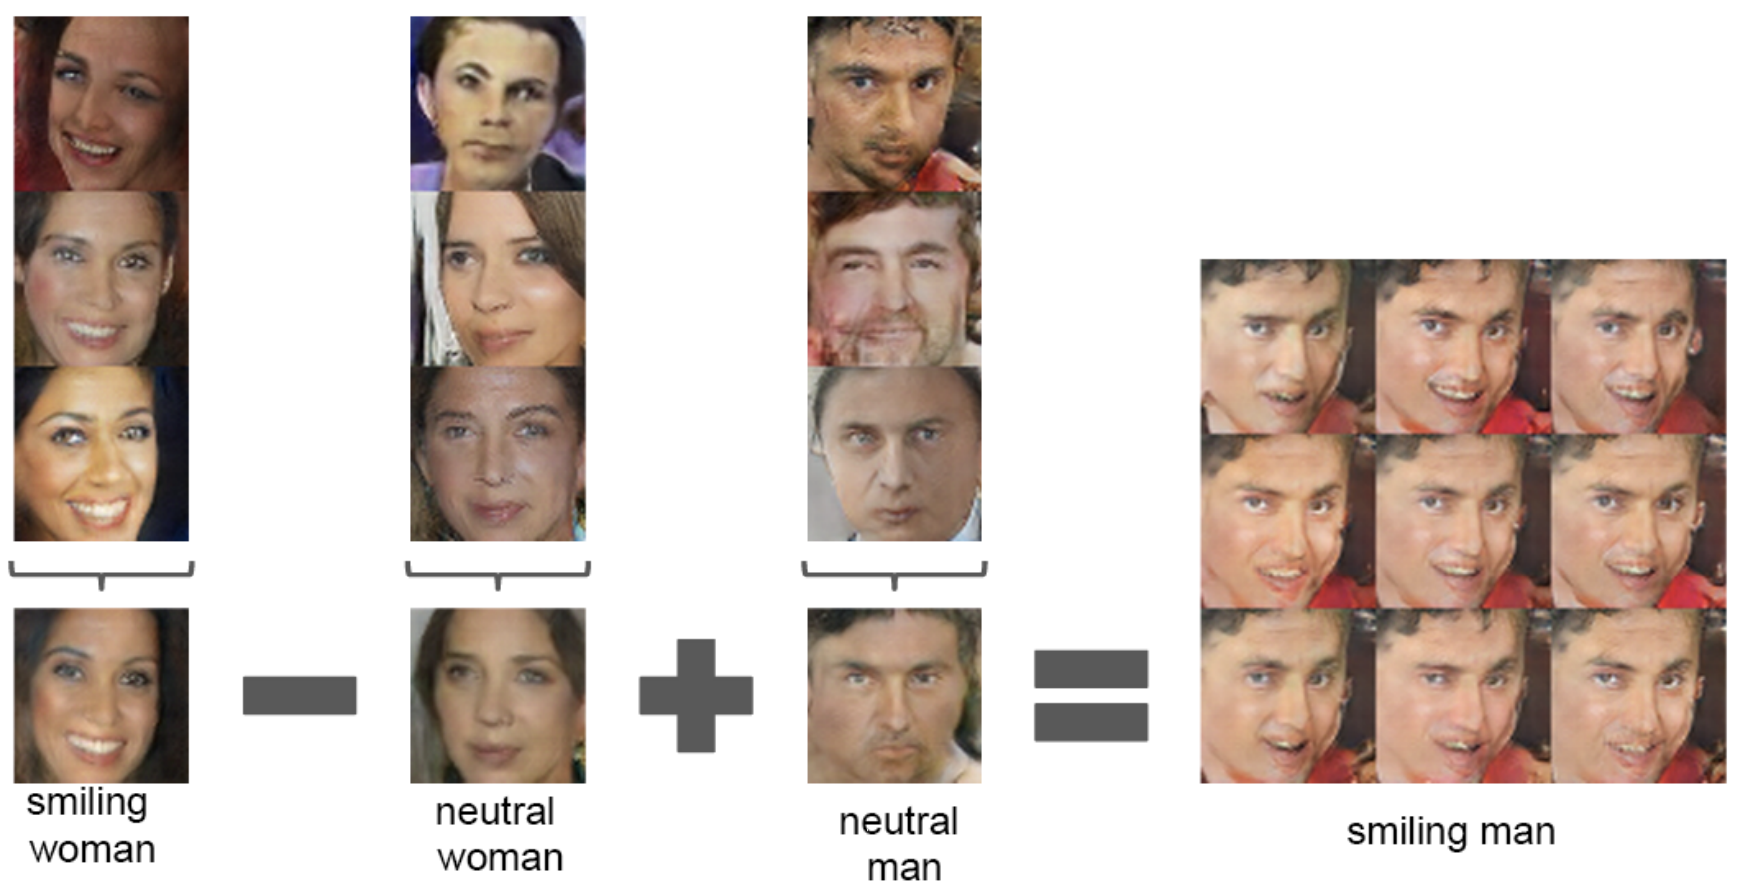
\includegraphics[width=1.0\linewidth]{figs/dcgan_results_3}
		\end{figure}
	\end{block}

	\myfootnotewithlink{https://arxiv.org/abs/1511.06434}{Radford A., Metz L., Chintala S. Unsupervised Representation Learning with Deep Convolutional Generative Adversarial Networks, 2015}
\end{frame}
%=======
\subsection{Improved techniques for training GANs}
%=======
\begin{frame}{Improved techniques for training GANs}
	\begin{itemize}
		\item Feature matching
		\[
			\cL_G = \| \bbE_{\pi(\bx)} \mathbf{d}(\bx) - \bbE_{p(\bz)} \mathbf{d}(G(\bz)) \|_2^2
		\]
		Here $\mathbf{d}(\bx)$ -- intermediate layer of discriminator. Matching the learned discriminator statistics instead of the output of the discriminator. Helps to avoid the vanishing gradients for sufficiently good discriminator.
		\item Historical averaging adds extra loss term for generator and discriminator losses
		\vspace{-0.2cm}
		\[
		 \| \btheta - \frac{1}{T}\sum_{t=1}^T \btheta_t\|^2_2.
		\]
		Here $\btheta_t$ -- value of parameters at the previous step $t$. It allows to stabilize training procedure.
	\end{itemize}
	\myfootnotewithlink{https://arxiv.org/abs/1606.03498}{Salimans T. et al. Improved Techniques for Training GANs, 2016}
\end{frame}
%=======
\begin{frame}{Improved techniques for training GANs}
	\begin{itemize}
		\item One-sided label smoothing. Instead of using one-hot labels in classification, use $(1 - \alpha)$ for real data (the generated samples are not smoothed).
		\[
			D^*(\bx) = \frac{(1 - \alpha )\pi(\bx)}{\pi(\bx) + p(\bx | \btheta)}
		\]
		\item Virtual batch normalization. BatchNorm makes samples within minibatch are highly correlated.
		\begin{figure}
			\centering
			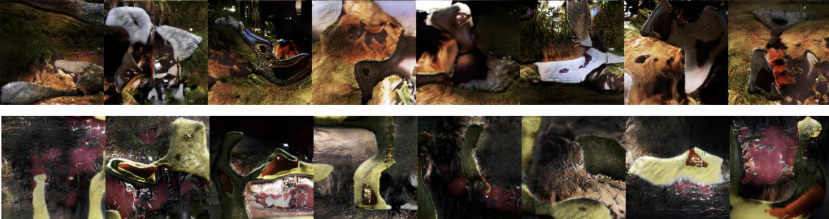
\includegraphics[width=0.6\linewidth]{figs/virtual_batch_norm}
		\end{figure}
	Use reference fixed batch to compute the normalization statistics. To avoid overfitting construct batch with the reference batch and the current sample. 
	\end{itemize}
	\myfootnotewithlink{https://arxiv.org/abs/1606.03498}{Salimans T. et al. Improved Techniques for Training GANs, 2016}
\end{frame}
%=======
\subsection{WGAN}
%=======
\begin{frame}{Wasserstein GAN}
	\begin{figure}
		\centering
		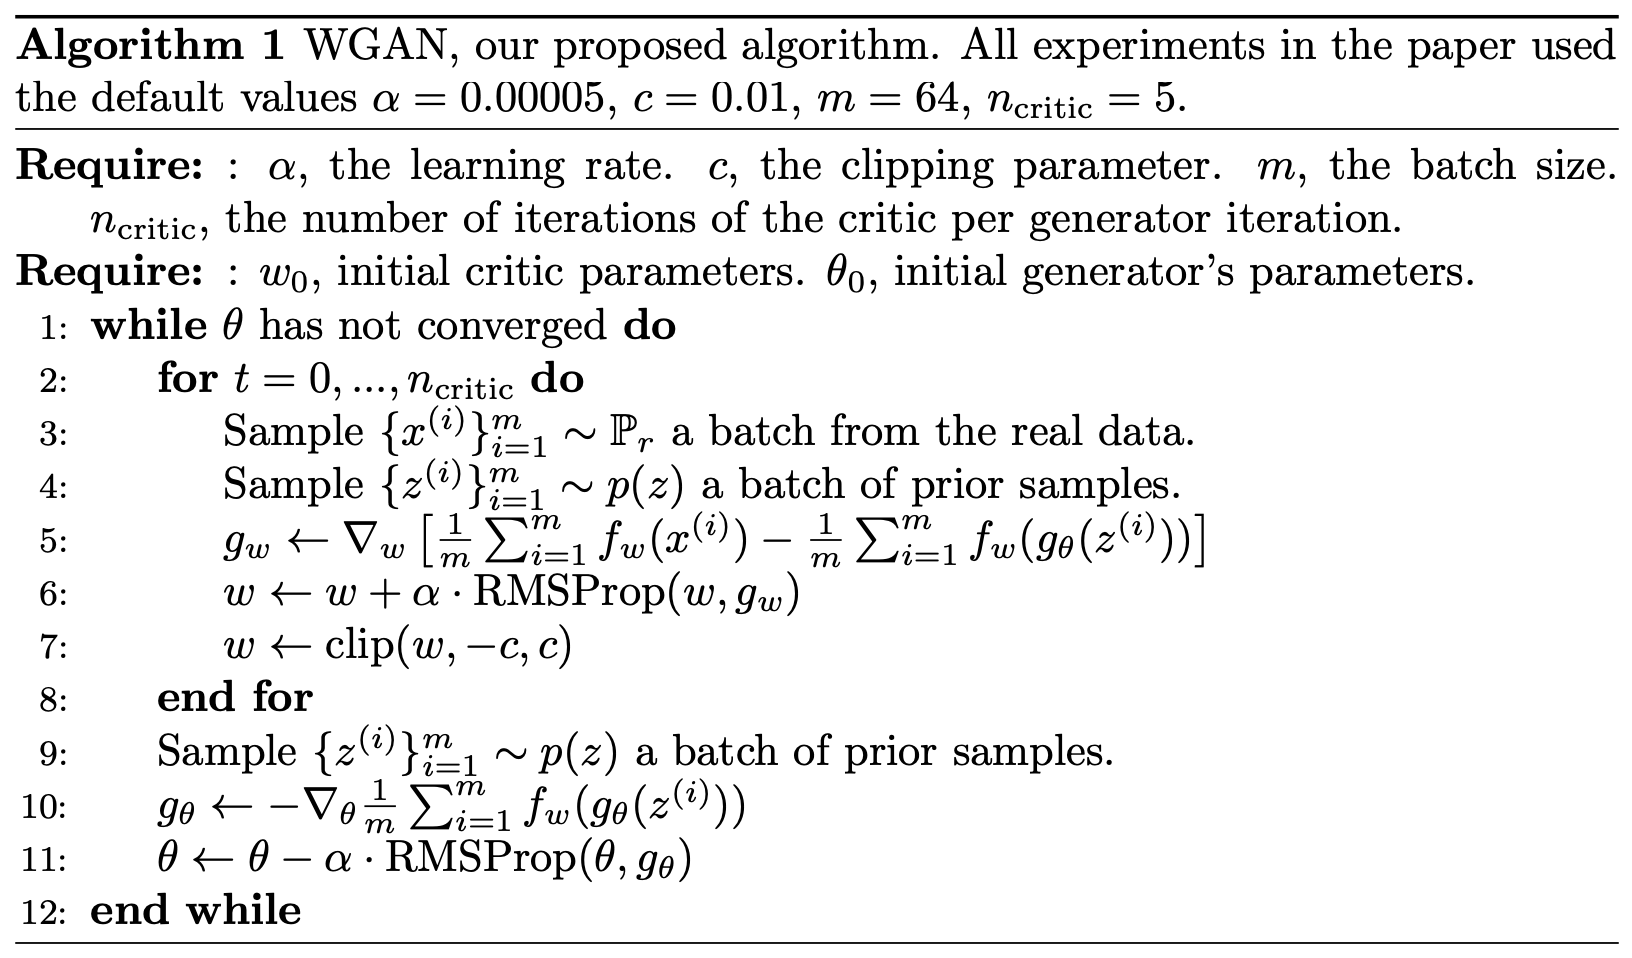
\includegraphics[width=1.0\linewidth]{figs/wgan_pseudocode}
	\end{figure}

	\myfootnotewithlink{https://arxiv.org/abs/1701.07875}{Arjovsky M., Chintala S., Bottou L. Wasserstein GAN, 2017}
\end{frame}
%=======
\begin{frame}{Wasserstein GAN with Gradient Penalty}
	
	\begin{figure}
		\centering
		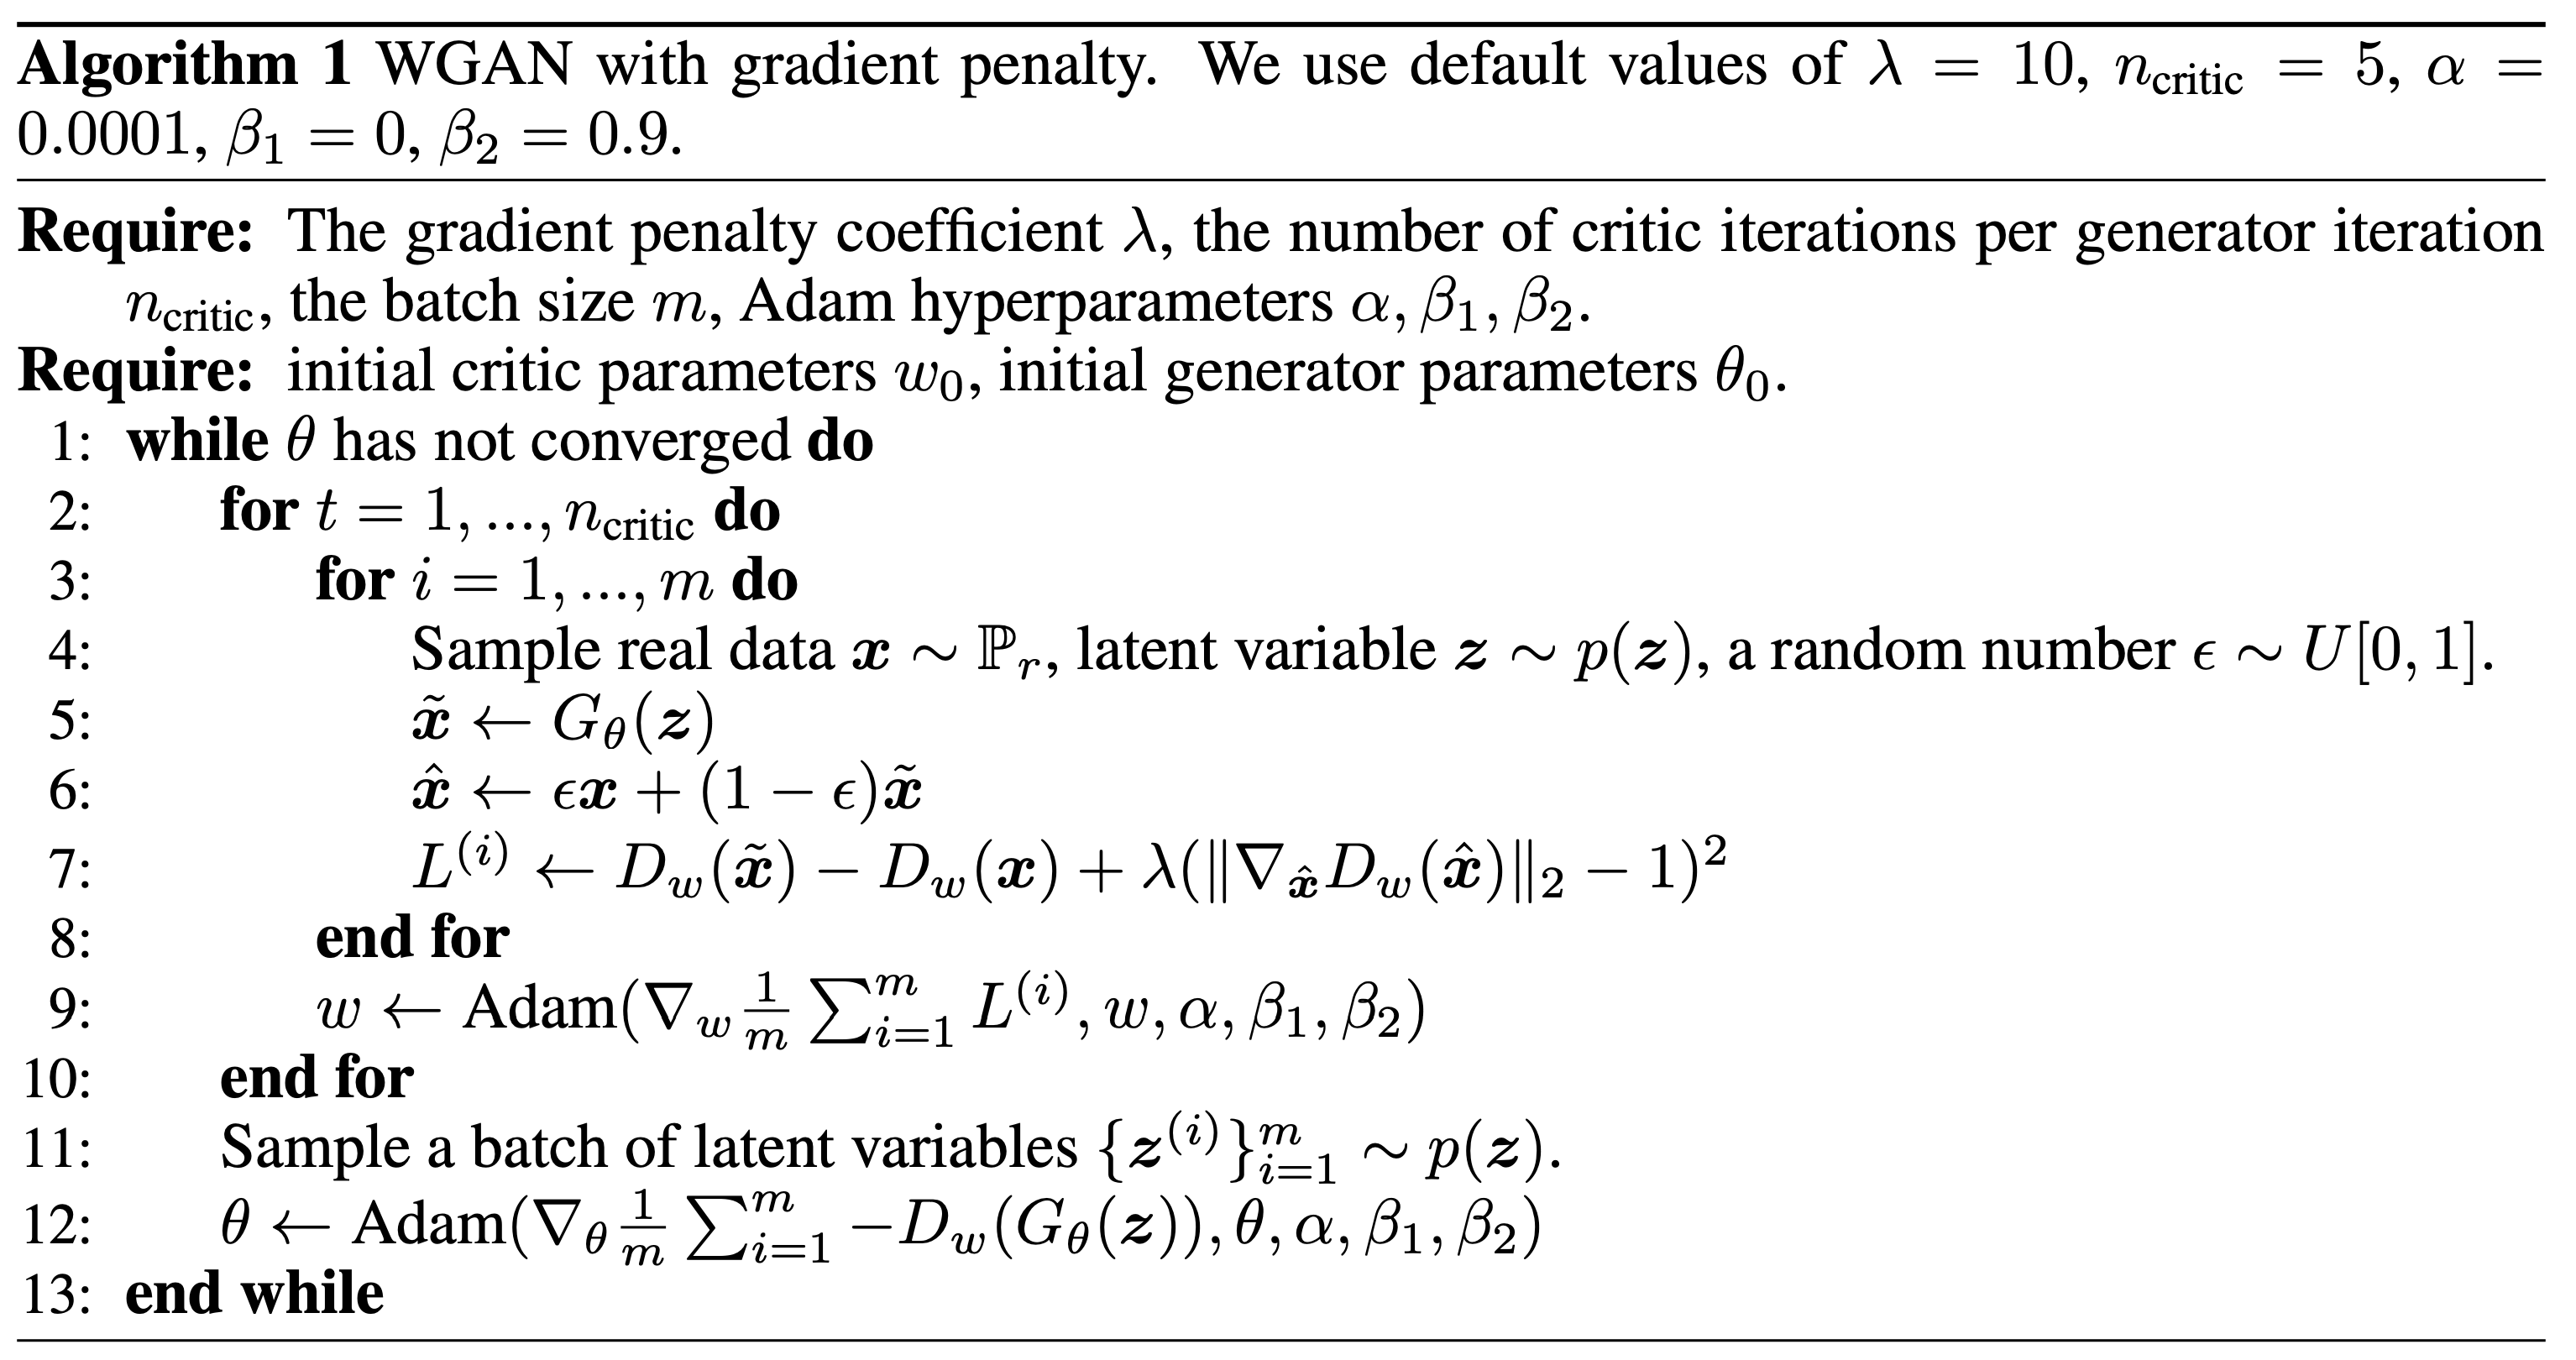
\includegraphics[width=1.0\linewidth]{figs/wgan_gp_pseudocode}
	\end{figure}

	\myfootnotewithlink{https://arxiv.org/abs/1704.00028}{Gulrajani I. et al. Improved Training of Wasserstein GANs, 2017}
\end{frame}
%=======
\subsection{StyleGAN}
%=======
\begin{frame}{StyleGAN}
	\begin{block}{Step 2: Style modulation}
		\begin{itemize}
			\item Adaptive Instance Normalization transfers the $\bw$ vector to the synthesis Network.
			\item The module is added to each resolution to define the visual expression of the features.
		\end{itemize}
		\begin{figure}
			\centering
			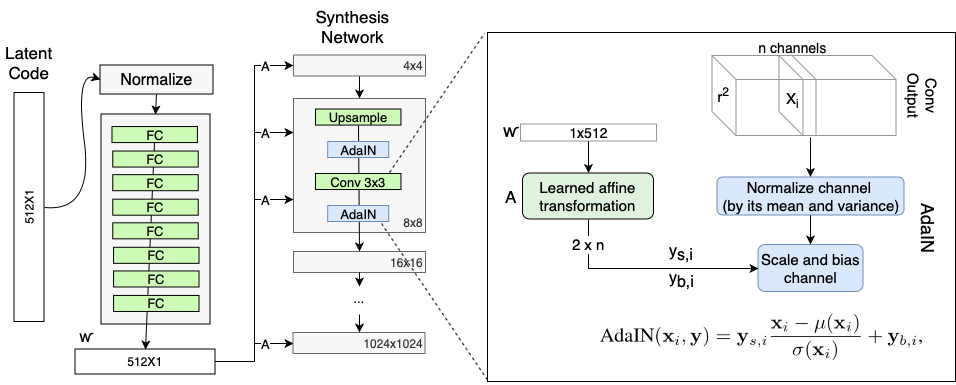
\includegraphics[width=1.0\linewidth]{figs/stylegan_adain}
		\end{figure}
	\end{block}

	\myfootnotewithlink{https://arxiv.org/abs/1812.04948}{Karras T., Laine S., Aila T. A Style-Based Generator Architecture for Generative Adversarial Networks, 2018}
\end{frame}
%=======
\begin{frame}{StyleGAN}
	\begin{block}{Step 3: Remove traditional input}
		Mapping network provides stochasticity to different stages of the synthesis network. Input of the synthesis network is a trainable vector.
		\begin{figure}
			\centering
			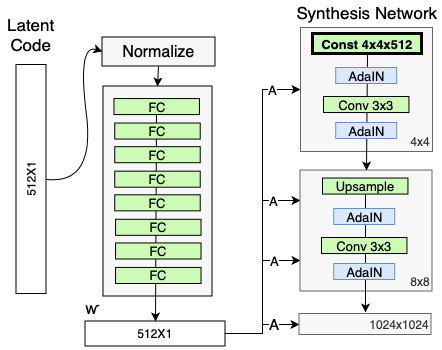
\includegraphics[width=0.55\linewidth]{figs/stylegan_input}
		\end{figure}
	\end{block}

	\myfootnotewithlink{https://arxiv.org/abs/1812.04948}{Karras T., Laine S., Aila T. A Style-Based Generator Architecture for Generative Adversarial Networks, 2018}
\end{frame}
%=======
\begin{frame}{StyleGAN}
	\begin{block}{Step 4: Stochastic variation}
		Inject random noise to add small aspects, such as freckles, exact placement of hairs, wrinkles, features which make the image more realistic and increase the variety of outputs.
		\begin{figure}
			\centering
			\includegraphics[width=0.9\linewidth]{figs/stylegan_noise}
		\end{figure}
	\end{block}

	\myfootnotewithlink{https://arxiv.org/abs/1812.04948}{Karras T., Laine S., Aila T. A Style-Based Generator Architecture for Generative Adversarial Networks, 2018}
\end{frame}
%=======
\begin{frame}{StyleGAN}
	\begin{block}{Step 4: Style Mixing}
		\vspace{-0.33cm}
		\begin{figure}
			\centering
			\includegraphics[width=0.8\linewidth]{figs/stylegan_mix_reg}
		\end{figure}
	\begin{itemize}
		\item Makes different levels of synthesis network to be independent.
		\item Allows to couple diffirent styles.
	\end{itemize}
	\end{block}

	\myfootnotewithlink{https://arxiv.org/abs/1812.04948}{Karras T., Laine S., Aila T. A Style-Based Generator Architecture for Generative Adversarial Networks, 2018}
\end{frame}
%=======
\begin{frame}{StyleGAN}
	\begin{figure}
		\centering
		\includegraphics[width=0.8\linewidth]{figs/stylegan_scheme}
	\end{figure}

	\myfootnotewithlink{https://arxiv.org/abs/1812.04948}{Karras T., Laine S., Aila T. A Style-Based Generator Architecture for Generative Adversarial Networks, 2018}
\end{frame}
%=======
\begin{frame}{StyleGAN}
		\begin{figure}
			\centering
			\includegraphics[width=0.6\linewidth]{figs/stylegan_mix}
		\end{figure}

	\myfootnotewithlink{https://arxiv.org/abs/1812.04948}{Karras T., Laine S., Aila T. A Style-Based Generator Architecture for Generative Adversarial Networks, 2018}
\end{frame}
%=======
\section{FFJORD}
%=======
\begin{frame}{Continuous Normalizing Flows}
	\begin{block}{Forward transform + log-density}
		\vspace{-0.8cm}
		\[
			\begin{bmatrix}
				\bx \\
				\log p(\bx | \btheta)
			\end{bmatrix}
			= 
			\begin{bmatrix}
				\bz \\
				\log p(\bz)
			\end{bmatrix} + 
			\int_{t_0}^{t_1} 
			\begin{bmatrix}
				f(\bz(t), \btheta) \\
				- \text{trace} \left( \frac{\partial f(\bz(t), \btheta)}{\partial \bz(t)} \right) 
			\end{bmatrix} dt.
		\]
		\vspace{-0.4cm}
	\end{block}
	\begin{itemize}
		\item Discrete-in-time normalizing flows need invertible $f$. It costs $O(d^3)$ to get determinant of Jacobian.
		\item Continuous-in-time flows require only smoothness of $f$. It costs $O(d^2)$ to get trace of Jacobian.
	\end{itemize}
	It is possible to reduce cost from $O(d^2)$ to $O(d)$!
	\begin{block}{Hutchinson's trace estimator}
		\vspace{-0.3cm}
		\[
		    \text{trace}(A) = \mathbb{E}_{p(\bepsilon)} \left[ \bepsilon^T A \bepsilon \right]; \quad \mathbb{E} [\bepsilon] = 0; \quad \text{Cov} (\bepsilon) = I.
		\]
		\vspace{-0.5cm}
	\end{block}
	\begin{block}{FFJORD density estimation}
		\vspace{-0.4cm}
		\[
		    \log p(\bz(t_1)) = \log p(\bz(t_0)) - \mathbb{E}_{p(\bepsilon)} \int_{t_0}^{t_1} \left[ \bepsilon^T \frac{\partial f}{\partial \bz} \bepsilon \right] dt.
		\]
	\end{block}
	\myfootnotewithlink{https://arxiv.org/abs/1810.01367}{Grathwohl W. et al. FFJORD: Free-form Continuous Dynamics for Scalable Reversible Generative Models, 2018} 
\end{frame}
%=======
\begin{frame}{FFJORD}
	\begin{figure}
		\centering
		\includegraphics[width=0.75\linewidth]{figs/flow_comparison.png}
	\end{figure}
	\vspace{-0.4cm}
	\begin{block}{Density estimation (forward KL)}
		\vspace{-0.2cm}
		\begin{figure}
			\centering
			\includegraphics[width=0.8\linewidth]{figs/ffjord_forward}
		\end{figure}
		\vspace{-0.5cm}
	\end{block}
	\begin{block}{Flows for variational inference (reverse KL)}
		\vspace{-0.2cm}
		\begin{figure}
			\centering
			\includegraphics[width=0.8\linewidth]{figs/ffjord_reverse}
		\end{figure}
	\end{block}

	\myfootnotewithlink{https://arxiv.org/abs/1810.01367}{Grathwohl W. et al. FFJORD: Free-form Continuous Dynamics for Scalable Reversible Generative Models, 2018} 
\end{frame}
%=======
\section{Vector Quantized VAE-2}
%=======
\begin{frame}{Vector Quantized VAE}
	\begin{itemize}
		\item The prior distribution over the discrete latents $p(\hat{\bz})$ is a categorical distribution.
		\item It could be made autoregressive by depending on other $\hat{\bz}$ in the feature map. 
		\item While training the VQ-VAE, the prior is kept constant and uniform. 
		\item After training, fit an autoregressive distribution (using PixelCNN) over $\hat{\bz}$.
	\end{itemize}
	\begin{block}{Samples}
		\begin{figure}
			\centering
			\includegraphics[width=\linewidth]{figs/vqvae_results}
		\end{figure}
	\end{block}

	\myfootnotewithlink{https://arxiv.org/abs/1711.00937}{Oord A., Vinyals O., Kavukcuoglu K. Neural Discrete Representation Learning, 2017} 
\end{frame}
%=======
\begin{frame}{Vector Quantized VAE-2}
	\begin{itemize}
		\item Use multi-scale hierarchical model.
		\item Use autoregressive prior model in each scale of the hierarchy.
		\item Improve autoregressive prior (PixelSNAIL with self-attention in bottom layer, PixelCNN++ in bottom layer).
		\item Train the encoder and decoder at the first stage, train the priors at the second stage.
	\end{itemize}
	\begin{figure}
		\centering
		\includegraphics[width=\linewidth]{figs/vqvae2}
	\end{figure}
	\myfootnotewithlink{https://arxiv.org/abs/1906.00446}{Razavi A., Oord A., Vinyals O. Generating Diverse High-Fidelity Images with VQ-VAE-2, 2019} 
\end{frame}
%=======
\begin{frame}{Vector Quantized VAE-2}
		\begin{figure}
			\centering
			\includegraphics[width=0.9\linewidth]{figs/vqvae2_pseudo}
		\end{figure}
		\vspace{-0.2cm}
		\begin{figure}
			\centering
			\includegraphics[width=0.85\linewidth]{figs/vqvae2_latents}
		\end{figure}
	\myfootnotewithlink{https://arxiv.org/abs/1906.00446}{Razavi A., Oord A., Vinyals O. Generating Diverse High-Fidelity Images with VQ-VAE-2, 2019} 
\end{frame}
%=======
\section{Feature Quantized GAN}
%=======
\begin{frame}{Feature Quantized GAN}
	\begin{itemize}
		\item GAN tries to find Nash equilibrium, minibatch training is unstable. GAN relies heavily on the minibatch statistics.
		\item Lots of feature matching strategies were proposed to stabilize the training. 
	\end{itemize}
	\begin{block}{Feature quantized GAN discriminator}
		\[
			D(\bx) = f_{\bw_T} \circ f_{\bw_B}(\bx) \quad \Rightarrow \quad D(\bx) = f_{\bw_T} \circ f_Q \circ f_{\bw_B}(\bx). 
		\]
	\end{block}
	Here $f_Q$ is a vector quantization operation.
	\begin{figure}
		\centering
		\includegraphics[width=0.7\linewidth]{figs/fqgan}
	\end{figure}
	\myfootnotewithlink{https://arxiv.org/abs/2004.02088}{Zhao Y. et al. Feature Quantization Improves GAN Training, 2020} 
\end{frame}
%=======
\begin{frame}{Feature Quantized GAN}
	\begin{block}{Quantization procedure}
		\begin{minipage}[t]{0.65\columnwidth}
			\begin{figure}
				\centering
				\includegraphics[width=\linewidth]{figs/fqgan_cnn.png}
			\end{figure}
		\end{minipage}%
		\begin{minipage}[t]{0.35\columnwidth}
			\begin{figure}
				\centering
				\includegraphics[width=0.9\linewidth]{figs/fqgan_lookup}
			\end{figure}
		\end{minipage}
	\end{block}
	\begin{block}{Quantized features}
		\begin{figure}
			\centering
			\includegraphics[width=\linewidth]{figs/fqgan_features}
		\end{figure}
	\end{block}
	\myfootnotewithlink{https://arxiv.org/abs/2004.02088}{Zhao Y. et al. Feature Quantization Improves GAN Training, 2020} 
\end{frame}
%=======
\begin{frame}{Feature Quantized GAN}
		\begin{minipage}[t]{0.45\columnwidth}
			\begin{block}{ImageNet-1000}
				\begin{figure}
					\centering
					\includegraphics[width=\linewidth]{figs/fqgan_results1.png}
				\end{figure}
			\end{block}
			\begin{block}{FFHQ}
				\begin{figure}
					\centering
					\includegraphics[width=\linewidth]{figs/fqgan_results2.png}
				\end{figure}
			\end{block}
		\end{minipage}%
		\begin{minipage}[t]{0.55\columnwidth}
			\begin{block}{Per class metrics for ImageNet}
				\begin{figure}
					\centering
					\includegraphics[width=\linewidth]{figs/fqgan_results3}
				\end{figure}
			\end{block}
		\end{minipage}
	\myfootnotewithlink{https://arxiv.org/abs/2004.02088}{Zhao Y. et al. Feature Quantization Improves GAN Training, 2020} 
\end{frame}
%=======
\end{document} 